
%----------------------------------------------------------------------------
\documentclass[a4paper,11pt]{article}
%----------------------------------------------------------------------------

%----------------------------------------------------------------------------
%% Language and font encodings
%----------------------------------------------------------------------------
\usepackage[a4paper,top=3cm,bottom=2cm,left=3cm,right=3cm,marginparwidth=1.75cm]{geometry}
\usepackage{graphicx} 
\usepackage[hidelinks]{hyperref} 
\usepackage{multirow} 
\usepackage{tabularx} 
\usepackage{color} 

\usepackage[fleqn]{amsmath}
\usepackage{amsfonts}
\usepackage{amssymb}
\usepackage{textcomp}
\usepackage{gensymb}

\usepackage{array}

\setlength\parindent{0pt}

\usepackage{amsxtra} 

\usepackage{wasysym} 
\usepackage{isomath} 
\usepackage{mathtools} 
\usepackage{txfonts} 
\usepackage{upgreek} 
\usepackage{enumerate} 
\usepackage{tensor} 
\usepackage{pifont} 
\usepackage{titlesec}

\usepackage[utf8x]{inputenc}
\usepackage[T1]{fontenc}
\usepackage{fancyhdr}
%\usepackage{enumitem}
%\usepackage[colorlinks=true, allcolors=blue]{hyperref}
%\usepackage{subcaption}

\usepackage[normalem]{ulem} %25/05
\usepackage{caption}%04/06
\usepackage{afterpage}%04/6

\usepackage{geometry}%05/06

\usepackage{wrapfig}%04/06
\usepackage{float}
%\usepackage[printfigures]{endfloat}
%\usepackage{endfloat}
\usepackage{subfig}
%\usepackage{graphicx}
%package floatend

\usepackage{booktabs}
\newcommand{\nhi}[1]{%
	{\itshape \color{magenta} (NHI approx: {#1})}
}
\newcommand{\hi}[1]{%
	{\itshape \color{cyan} (HI approx: {#1})}
}
%----------------------------------------------------------------------------
% Packages: uncomment to debug
%----------------------------------------------------------------------------
%\usepackage{refcheck}
\renewcommand{\labelitemi}{\textbullet}

%----------------------------------------------------------------------------
% Packages: bibliography
%----------------------------------------------------------------------------
\usepackage[nottoc, notlof, notlot]{tocbibind}
%\usepackage[authoryear, round]{natbib}
\usepackage[authoryear]{natbib}

\usepackage[english]{babel}

\usepackage{authblk}

\DeclareMathOperator{\cotan}{cotan}


%----------------------------------------------------------------------------
% Colors...
%----------------------------------------------------------------------------
\definecolor{color-1}{rgb}{0.21,0.37,0.57}
\definecolor{color-2}{rgb}{0.31,0.51,0.74}

%----------------------------------------------------------------------------
\titleformat*{\section}{\large\bfseries}
\titleformat*{\subsection}{\normalfont\bfseries}
%\title{A unified theory of acoustic and gravity waves in a compressible stratified ocean}
\title{Theory and analysis of acoustic-gravity waves in a free-surface compressible and stratified ocean}


%----------------------------------------------------------------------------
\geometry{hmargin=2.5cm,vmargin=2.5cm} %marges
%----------------------------------------------------------------------------


%%%%%%%%%%%%%%%%%%%%%%%%%%%%%%%%%%%%%%%%%%%%%%%%%%%%%%%%%%%%%%%%%%%%%%%%%%%
\author[1]{F. Auclair\thanks{Corresponding author: francis.auclair@aero.obs-mip.fr}}
\author[2]{L. Debreu}
\author[2]{E. Duval}
\author[3]{P. Marchesiello}
\author[2]{E. Blayo}
\author[1]{M. Hilt}

%\author[5]{P. Marchesiello}
%\author[1]{C. Nguyen}
%\author[1]{L. Roblou}
%\author[affilINRIA]{F. Lemari\'e}
%\author[affilIFREMER]{S. Jullien}
%\author[affilSHOM]{L. Bordois}
%\author[affilLEGOSCNRS]{R. Benshila}
%
\affil[1]{Laboratoire d'A\'erologie, Universit\'e de Toulouse, CNRS, UPS, France}
%\affil[2]{IPSL/LOCEAN, CNRS, UPMC, IRD, MNHN, France}
\affil[2]{Univ. Grenoble Alpes, Inria, CNRS, Grenoble INP, LJK, 38000 Grenoble, France}
%\affil[4]{Service Hydrographie et Oc\'eanographie de la Marine, Brest, France}
\affil[3]{LEGOS, IRD, Universit\'e de Toulouse, CNRS, CNES, France}
%
%\address[affilLEGOSCNRS]{LEGOS/CNRS, 31400 Toulouse, France}
%\address[affilIFREMER]{Ifremer, Univ. Brest, CNRS, IRD, Laboratoire d'Océanographie Physique et Spatiale (LOPS), IUEM, F- 29280, Plouzan\'e, France}
%
%%%%%%%%%%%%%%%%%%%%%%%%%%%%%%%%%%%%%%%%%%%%%%%%%%%%%%%%%%%%%%%%%%%%%%%%%%%

%%%%%%%%%%%%%%%%%%%%%%%%%%%%%%%%%%%%%%%%%%%%%%%%%%%%%%%%%%%%%%%%%%%%%%%%%%%%
\begin{document}
%%%%%%%%%%%%%%%%%%%%%%%%%%%%%%%%%%%%%%%%%%%%%%%%%%%%%%%%%%%%%%%%%%%%%%%%%%%%%
%\bibliographystyle{agsm}

\renewcommand{\thepage}{}
\hypersetup{pdfborder=0 0 0}
\maketitle
\setcounter{tocdepth}{2}

%----------------------------------------------------------------------------
% \ref with ( )
%----------------------------------------------------------------------------
\let\oldref\ref
\renewcommand{\ref}[1]{(\oldref{#1})}

%%%%%%%%%%%%%%%%%%%%%%%%%%%%%%%%%%%%%%%%%%%%%%%%%%%%%%%%%%%%%%%%%%%%%%%%%%%%%
%\tableofcontents
%%%%%%%%%%%%%%%%%%%%%%%%%%%%%%%%%%%%%%%%%%%%%%%%%%%%%%%%%%%%%%%%%%%%%%%%%%%%%

%%%%%%%%%%%%%%%%%%%%%%%%%%%%%%%%%%%%%%%%%%%%%%%%%%%%%%%%%%%%%%%%%%%%%%%%%%%%%
% Abstract
%%%%%%%%%%%%%%%%%%%%%%%%%%%%%%%%%%%%%%%%%%%%%%%%%%%%%%%%%%%%%%%%%%%%%%%%%%%%%
\textit{Abstract:} Waves propagate in a free-surface ocean due to compressibility and gravity (and surface tension at much smaller scale). Analytical solutions have long been derived independently for acoustic and gravity waves, i.e., acoustic waves or internal-gravity rays in an unbounded ocean, surface-gravity waves in a free-surface-ocean, and acoustic or internal modes in a bounded ocean. In the present study, capillarity waves and earth-rotation are neglected and a simple, unified model based on inner and boundary dispersion relations is derived for waves propagating in a compressible, stratified, free-surface ocean. Wave solutions are identified and visually analyzed in phase-space. Taylor developments are then carried out with respect to small parameters describing stratification and compressibility and are compared with numerical approximations of the intersection of inner and boundary dispersion surfaces. Finally, the model recovers the known approximations for swell, long-surface waves, internal-gravity rays, internal modes, acoustic waves or acoustic modes, and also provides modification of these solutions due to stratification and compressibility.\\

%%%%%%%%%%%%%%%%%%%%%%%%%%%%%%%%%%%%%%%%%%%%%%%%%%%%%%%%%%%%%%%%%%%%%%%%%%%
\newpage
\renewcommand{\thepage}{\arabic{page}}
\setcounter{page}{1}
%%%%%%%%%%%%%%%%%%%%%%%%%%%%%%%%%%%%%%%%%%%%%%%%%%%%%%%%%%%%%%%%%%%%%%%%%%%%%
\section{Introduction}
%%%%%%%%%%%%%%%%%%%%%%%%%%%%%%%%%%%%%%%%%%%%%%%%%%%%%%%%%%%%%%%%%%%%%%%%%%%%%
Many types of waves are known to propagate in the ocean, and textbooks \citep{LeBlond_Mysak_1981, gill_1982, Pedlosky_1982} have detailed the derivation of their analytical solutions for decades. These waves can be classified in several categories depending on the type of mechanisms directly involved in their propagation. Neglecting Earth's rotation and associated planetary waves, two fundamental categories are of particular interest in the present study: acoustic (sound) waves, which are a consequence of ocean compressibility, and gravity waves, which are sustained by the gravity force. Table \oldref{TableWave solutions} gives a short (and necessarily incomplete) list of such waves. A particular type of waves is most often characterized by a space-time dispersion relation, linking its time frequency (or period) with its space wavenumber (or wavelength). The phase and group velocities and wave dispersion capacity can be derived from the dispersion relations.

If ocean waves are short enough and generated far enough from the surface and bottom boundaries, they can propagate in the ocean as in any unbounded medium. However, when they are generated in the vicinity of these boundaries or when their wavelengths are large compared to the ocean depth, ocean waves are known to take specific forms, and the ocean basin is a \textit{wave-guide} propagating \textit{wave modes}. For example, the ocean stratification introduces internal gravity modes with "long" horizontal wavelengths. Another example are acoustic modes which are associated with compressibility effects and which have been recently re-discovered \citep{smith_2015}. Such internal and acoustic waves are qualified as "modes" since their vertical wavelength is constrained by the vertical extend of the domain. The ocean free-surface is permanently shaken by a myriad of horizontally propagating waves and it is not always clear whether these waves are modes or just vertically-evanescent edge-waves. Capillary waves, swells, tidal waves, tsunamis are well-known examples of such free surface waves.

Deriving a dispersion relation for acoustic waves or for internal wave rays in an unbounded ocean is rather straightforward. The method generally includes two steps: small amplitude is assumed; only specific wave-restoring mechanisms and medium characteristics are retained in the simplest possible wave dispersion model (compressibility and pressure force for acoustic waves, gravity and vertical advection of isopycnal surfaces for internal waves). The linear nature of the resulting model has two main advantages: analytical solutions can be derived and waves can be superimposed without interaction \citep{lighthill_1967}.

The introduction of free-surface brings more complexity. Small-amplitude is usually postulated in this case also and both gravity and free-surface motions are retained in the dispersion model. However, surface waves are "edge waves" propagating at the interface between the atmosphere and the ocean, and the surface kinematic relation (the free-surface general boundary condition) leads to a transcendental dispersion relation with trigonometric terms. As a result, deriving analytical solutions requires further simplifications. Specific analytical solutions can then be found in the literature depending, for example, on  relative depth, .i.e., the product of horizontal wavenumber $k_x$ and ocean depth $H$ (Table \oldref{TableWave solutions}). Long gravity wave solutions are a particular case of small $k_x H$, well-known to propagate horizontally with $\sqrt{g H}$ phase and group velocities (where $g$ is the acceleration of gravity).

%%%%%%  DIFF 1 %%%%%
%%%%%%%%%%%%%%%%%%%%%%%%%%%
% Table  Wave solutions
%%%%%%%%%%%%%%%%%%%%%%%%%%%

%%%%%%%%%%%%%%%%%%%%%%%%%%%%%%%%%%%%%%%%%%%%%%%%%
% Version Laurent ... ne passe pas git-latexdiff
%%%%%%%%%%%%%%%%%%%%%%%%%%%%%%%%%%%%%%%%%%%%%%%%%
%\newcolumntype{P}[1]{>{\centering\arraybackslash}p{#1}}
\begin{table}[!h]
	\setlength{\extrarowheight}{15pt}
		\centerline{
	\begin{tabular} {p{3.8cm}|p{4.7cm}|c|p{3.8cm}}
		Waves & Assumptions & Frequency $(\Omega)$ & Vertical wavenumber $k_z$\\
		\hline\hline
		Acoustic waves & Compressible, unbounded &$\Omega_{aw}^2=c_s^2(k_x^2+k_z^2)$& \\
		Internal gravity rays & Stratified, unbounded &$\displaystyle \Omega_{iwr}^2=\frac{N^2 k_x^2}{k_x^2+k_z^2}$ &  \\\hline
		Acoustic gravity modes & Compressible, bounded &$\Omega_{am}^2=c_s^2(k_x^2+k_z^2)$&$\displaystyle k_{z,am}=\frac{\pi}{2H}+\frac{m\pi}{H}$  \\
		Swell & Free-surface &$\Omega_{sw}^2=g k_x \tanh(k_x H)$ &$k_{z,sw}\approx k_x$  \\
		Long surface waves & Free-surface, shallow &$\Omega_{lsw}^2=gH\ k_x^2$ &$k_{z,lsw}\approx k_x$ \\
		Internal gravity modes & Stratified, bounded &$\displaystyle \Omega_{im}^2=\frac{N^2 k_x^2}{k_x^2+k_z^2}$&$\displaystyle k_{z,im}=\frac{n\pi}{H}$
		  \\
		%Low frequency Oscillations
		%(Long MIM, $n=0$) & Stratified, bounded & & 0\\
	\end{tabular}}	
	\caption{Simplified models of ocean waves and their dispersion relations in a vertical section, for an unbounded ocean (top) and for a bounded ocean (bottom). $\Omega$ is the time frequency of the wave, $k_x$ and $k_z$ are wavenumbers, $g$ is the acceleration of gravity, $H$ a reference depth, $N$ a reference Brunt-V\"ais\"al\"a frequency and $c_s$ the speed of sound. $n$ and $m$ are two positive integer numbers.}
	\label{TableWave solutions}
\end{table}
%%%%%%%%%%%%%%%%%%%%%%%%%%%%%%%%%%%%%%%%%%%%%%%%%

%\begin{table}[!h]
%	\setlength{\extrarowheight}{15pt}
%	\begin{tabular} {p{2.7cm}|p{3cm}|c|p{2.3cm}|p{3cm}}
%		Waves & Assumptions & Pulsation $(\Omega)$ & $k_z$ & Modified wave\\\hline
%		Acoustic waves & Compressible, unbounded &$\Omega_{aw}^2=c_s^2(k_x^2+k_z^2)$& & MAW \\
%		Internal gravity rays & Stratified, unbounded &$\Omega_{iwr}^2=\frac{N^2 k_x^2}{k_x^2+k_z^2}$ & & MIW \\\hline
%		Acoustic gravity modes & Compressible, bounded &$\Omega_{am}^2=c_s^2(k_x^2+k_z^2)$&$k_{z,am}=\frac{\pi}{2H}+\frac{m\pi}{H}$ & MAM \\
%		Swell & Free-surface &$\Omega_{sw}^2=g k_x tan(k_x H)$ &$k_{z,sw}\approx k_x$ & MSW \\
%		Long Surface waves & Free-surface, shallow &$\Omega_{lsw}^2=gH\ k_x^2$ &$k_{z,lsw}\approx k_x$& LMSW \\
%		Internal gravity modes & Stratified, bounded &$\Omega_{im}^2=\frac{N\pi}{nH}$&$k_{z,im}=\frac{n\pi}{H}$ & MIM \\
%		Low frequency Oscillations
%		(Long MIM, $n=0$) & Stratified, bounded & & & LMIM0\\
%	\end{tabular}
%	
%	\caption{examples of ocean waves and their dispersion relations in a vertical section. $\Omega$ is the pulsation of the wave, $k_x$ and $k_z$ are the wave-numbers, $g$ is the acceleration of gravity, $H$ a reference depth, $N$ a reference Brunt-V\"ais\"al\"a pulsation and $c_s$ the speed of sound. $n$ and $m$ are two positive integer numbers. For an unbounded ocean (top) and for a bounded ocean (bottom).}
%	\label{TableWave solutions}
%\end{table}
%%%%%%  DIFF 1 %%%%%

%%%%%%%%%%%%%%%%%%%%%%%%%%%
% Table 
%%%%%%%%%%%%%%%%%%%%%%%%%%%


%%%%%%%%%%%%%%%%%%%%%%%%%%%
% Table  AGWaves acronyms 22222
%%%%%%%%%%%%%%%%%%%%%%%%%%%
%\newcolumntype{P}[1]{>{\centering\arraybackslash}p{#1}}
%\begin{table}[!h]
%	\setlength{\extrarowheight}{15pt}
%	\begin{tabular} {c|c|c|c}
%		Acronym & Name & Dispersion relations & Parametrized relations \\\hline
%		MAW & Modified Acoustic Wave & \ref{DispAcousDT} & MAW \ref{DispAcousDT}\\
%		MIW & Modified Internal Wave ray & \ref{DispRaysDT} & MIW \ref{DispRaysDT}\\\hline
%		MAM & Modified Acoustic Mode $(m=1)$& (\oldref{EqFullDispera} \& \oldref{EqFullDisperb}) & MAM (\oldref{paramMAM1}, \oldref{paramMAM2}),\\
%		& & & LMAM (\oldref{ParamLMAM1}, \oldref{ParamLMAM2})\\
%		MSW & Modified Surface Wave & \ref{EqFullDisperai} \& \ref{EqFullDisperb} & MSW (\oldref{EqDispLonga1} \& \oldref{Eqdzdx2}) \\
%		LMSW & Long Modified Surface Wave & \ref{EqFullDisperai} \& \ref{EqFullDisperb} & LMSW (\oldref{Eqxxx} \& \oldref{EqDispDeltaz0}) \\
%		MIM & Modified Internal Mode $(n=1)$  & (\oldref{EqFullDispera} \& \oldref{EqFullDisperb}) & MIM (\oldref{ParamallMIM1}, \oldref{ParamallMIM2}),\\
%		& & & LMIM (\oldref{ParamMIM1}, \oldref{ParamMIM2})\\
%		LMIM0 & Long Gravity Oscillation (LMIM 0)& \ref{EqFullDispera} \& \ref{Eqxxx} & LMIM0 (\oldref{MIMomega2}, \oldref{MIMdz2})\\
%	\end{tabular}
%	
%	\caption{Acronyms of modified wave and modes.}
%	\label{TableWaveAcronyms}
%\end{table}
%%%%%%%%%%%%%%%%%%%%%%%%%%%
% Table 
%%%%%%%%%%%%%%%%%%%%%%%%%%%

%Such simplified models for small-amplitude waves are facing (at least) two severe limitations when compared to real-life ocean waves. Firstly, real ocean waves do not have an infinitesimal amplitude and finite-amplitude waves differ from their small-amplitude avatars: their non-linear growth can indeed lead to breaking or to new equilibrium when non-linearity can be counteracted by wave dispersion (propagating for instance as solitary waves). The second limitation comes from the fact that only specific wave-restoring mechanisms and medium characteristics are retained in process-oriented dispersion models whereas, in real ocean, compressibility can modify internal and surface waves and gravity can modify acoustic waves.
\newpage

The derivation of mixed acoustic-gravity waves in an ocean bounded by a free surface is even more challenging and is the central subject of this paper. The main objective is to specify the effect of compressibility and stratification on the preceding particular cases of wave solutions. Another target is to found analytical solutions to validate recent developments of the CROCO ocean model, resolving nonhydrostatic equations based on a pseudo-compressible approach \citep{AUCLAIR201812}.

\cite{ECKART1960136} provides one of the most comprehensive view of oceanic waves.
More recently \cite{dukowicz_2013} also tackled this problem and proposed a review of \textit{"Various approximations in atmosphere and ocean models based on an exact treatment of gravity wave dispersion"}. In that paper, acoustic-gravity waves were shown to satisfy a system of two dispersion relations and the impact of several usual assumptions of ocean models was evaluated. The present study builds on Eckart's and Dukowicz's results and more specifically focuses on the impact of both stratification and compressibility on acoustic-gravity wave solutions: Taylor expansions of dispersion relations and resulting expressions for wavelength and frequency are derived in terms of compressibility and stratification. In addition:
\begin{itemize}
%	\item We show that, when the Boussinesq approximation is not made, free-surface boundary constraints can be recovered at the same order of precision as in Dukowicz's but using an Eulerian framework.
	%We do not intent to show that the Eulerian framework makes more physical sense than the Lagrangian framework but just that it can reduce the analytical burden.
	\item A systematic graphic analysis of wave solutions is proposed in 3D frequency/wavenumber phase-space, unfolding their dependency to the vertical wavenumber. The graphic presentation allows us to synthesize all possible connections between usual acoustic, internal and surface wave solutions.
	\item Surface waves are systematically studied together with internal and acoustic modes.
	\item Long-wave solutions are investigated in details in order to better understand from which solution branch they asymptotically derive; approximate parametric relations are derived for each type of wave.
%	\item A particular region of phase space is identified where surface acoustic-gravity surface wave are "structurally singular" in the sense that gravity and compressibility are both important and the corresponding wave solution is close to instability in time.
\end{itemize}

In the section \oldref{SectionLinModels}, a linear model of ocean wave propagation is proposed with bottom and surface boundary conditions, and a corresponding system of two dispersion relations (which will be called {\it inner} and {\it boundary} dispersion relations) is derived. The inner dispersion relation, which does not take into account the bottom and surface boundary conditions, is studied in details in Section \oldref{SectionInner}, and the wave solutions propagating in an unbounded ocean are investigated. Waves propagating in a bounded ocean, which also have to satisfy the boundary relation dispersion, are then studied in Section \oldref{SectionGraphic}. Conclusions are drawn in Section \oldref{SectionDiscussion}.

%\newpage
%\textit{Objectives and novelty of the present study:}
%\begin{itemize}
%	\item general dispersion relations for acoustic and gravity waves,
%	\item modification of gravity (acoustic) waves by
%	\item (i) graphical study and identification of various wave solutions,
%	\item (ii) Taylor expansion of the inner and surface relations to compute wave solutions,
%	\item (iii) Taylor expansion of the identified wave solutions in terms of non-linearity and non-hydrostaticity.
%	\item tan and tanh surface solutions (transcendental).
%	\item analytical solutions in $\omega$ of the inner ocean dispersion relation.
%	\item comparison with classical solution.
%	\item numerical solutions of the intersections.
%\end{itemize}


%%%%%%%%%%%%%%%%%%%%%%%%%%%%%%%%%%%%%%%%%%%%%%%%%%%%%%%%%%%%%%%%%%%%%%%%%%%%%
%\newpage
%%%%%%%%%%%%%%%%%%%%%%%%%%%%%%%%%%%%%%%%%%%%%%%%%%%%%%%%%%%%%%%%%%%%%%%%%%%%%
\section{Linear model for surface and internal acoustic-gravity waves}
\label{SectionLinModels}
%%%%%%%%%%%%%%%%%%%%%%%%%%%%%%%%%%%%%%%%%%%%%%%%%%%%%%%%%%%%%%%%%%%%%%%%%%%%%

\subsection{General model for a compressible, viscous ocean}
\label{SubSectionNSModel}

Ocean dynamics can be described with a small number of macroscopic variables: velocity $(\mathbf{v})$, pressure and density ($p$ and $\rho$), temperature and salinity ($T$ and $S$). In a Cartesian framework, the general equations governing the motion of a compressible, viscous ocean are then:
{\color{red}PAS CORIOLIS}
%
\begin{subequations}
 \begin{alignat}{2}
 \displaystyle
 %%%%%%%%%%%%%% Continuity %%%%%%%%%%%%%%%%%
 \label{NS_a} 
 & \frac{\partial\rho}{\partial t} &&= - \mathbf{\nabla}\cdot(\rho \mathbf{v})\\[3mm]  
 %%%%%%%%%%%%%%%% Momentum %%%%%%%%%%%%%%%%%
 \label{NS_b}
	 & \frac{\partial \rho \mathbf{v}}{\partial t} 
	 &&= -\mathbf{\nabla}\cdot(\rho \mathbf{v}\otimes \mathbf{v}) 
	 -\mathbf{\nabla}p + 		
	\mathbf{\nabla}\cdot\underbrace{\left(
	\mu(\mathbf{\nabla}\mathbf{v}+\mathbf{\nabla}\mathbf{v}^{\ T})
 +\mu_2(\mathbf{\nabla}\cdot\mathbf{v})\ \mathbf{I}\ \right)}_{\mathbold{\tau}}
 +\rho \mathbf{g}\\
 %
 \label{NS_c}
 & \frac{\partial T}{\partial t} &&=-\mathbf{\nabla}\cdot(T\mathbf{v})
 +\mathbf{\nabla}\cdot\kappa_T\mathbf{\nabla}{T}\\[3mm]
 %
 \label{NS_d}
 & \frac{\partial S}{\partial t} &&=-\mathbf{\nabla}\cdot(S\mathbf{v})
 +\mathbf{\nabla}\cdot\kappa_S\mathbf{\nabla}{S}\\[3mm]
 \label{NS_e}
 & \rho &&= \rho(T,S,p)
 %
  \end{alignat}
\end{subequations}
%
where $\mathbf{I}$ is the identity matrix, superscript T indicates transposition, $\mu$ and $\mu_2$ are the kinetic and bulk (or second) viscosities, $\kappa_T$ and $\kappa_S$ are the heat and salt diffusivities. The first equations are written in a conservative form. They specify basic conservation principles: conservation of mass for Equation \ref{NS_a}, conservation of momentum for Equation \ref{NS_b} and conservation of heat and salt for equations \ref{NS_c} and \ref{NS_d}. Equation \ref{NS_e} is a functional relation describing the thermodynamic equation of state (EOS). 

\subsection{Surface and bottom boundary conditions}
\label{SubSectionBC}

At the bottom $(z=-H)$ and surface $(z=\zeta)$ of the ocean, boundary conditions must be specified for each variable (or for its derivatives). A simple condition of no penetration and no-slip at the ocean bottom can be written:
%
\begin{equation}
 \displaystyle
 \label{NS_BC0}
  \mathbf{v}(\mathbf{x_{\scriptscriptstyle H}},z=-H,t)=\mathbf{0}
\end{equation}
%
Neglecting surface-tension pressure drop, surface pressure is given by:
%
\begin{equation}
 \displaystyle
 \label{NS_BC1}
  p(\mathbf{x_{\scriptscriptstyle H}},z=\zeta,t)= p_{atm}
\end{equation}
%
with $p_{atm}$ the atmospheric pressure imposed at the surface of the ocean. Surface capillarity waves are consequently filtered out and will be neglected in the remaining of this work. The surface kinematic condition expresses the motion of the free-surface and relates the free-surface anomaly $\zeta$ to the surface vertical velocity $w$:
%
\begin{equation}
  \displaystyle
  \label{NS_BC2}
  \frac{\textrm{d}\zeta(\mathbf{x_{\scriptscriptstyle H}},t)}{\textrm{dt}}=w(\mathbf{x_{\scriptscriptstyle H}},z=\zeta,t)
\end{equation}
%
This kinematic boundary condition allows the propagation of surface gravity waves.

\subsection{Pressure and density decomposition and EOS simplification}
\label{SubSectionPRHO}

Waves are defined as small disturbances to a motionless thermodynamic equilibrium state, and both pressure and density can be decomposed into an equilibrium component and a small increment. In addition, as a first approximation, the impact of atmospheric pressure $p_{atm}$ can be neglected --- it can take an active part in wave generation, but only plays a minor role during propagation. 

The usual decomposition is now formalized for pressure \ref{decompoP_f} and density \ref{decompor_f}:
%
\begin{subequations}
  \begin{alignat}{2}
  % Pressure decomposition
  \displaystyle 
  \label{decompoP_f}
  \nonumber&p(\mathbf{x},t) &&= 
  \underbrace{\underbrace{p_{atm}
  (\mathbf{x_{\scriptscriptstyle H}},t)}_{\approx0}
  +g\int_z^{\zeta}\rho_{h}(\mathbf{x_{\scriptscriptstyle H}},z',t)\ dz'}_{p_h(\mathbf{x},t)}
  +\delta p(\mathbf{x},t)\\[3mm]
  & &&= \underbrace{
  \underbrace{g\int_z^{\zeta}{\displaystyle \hat{\rho}_h(z')}\ dz'}_{\hat{p}_h(z)}
  +\underbrace{g\int_z^{\zeta}{\left(\rho_{h}(\mathbf{x_{\scriptscriptstyle H}},z',t)-\hat{\rho}_h(z')\right)\ dz'}}
  _{p_h'(\mathbf{x},t)}}_{p_h(\mathbf{x},t)}
  +\, \delta p(\mathbf{x},t)\\[3mm]
  \label{decompor_f}  
  % Density decomposition
  \nonumber&\rho(\mathbf{x},t) &&=\underbrace{\hat{\rho}_{TS}(z)+\rho_{TS}'(\mathbf{x},t)}_{\rho_{TS}(\mathbf{x},t)=\rho(T,S,p=0)}
  +\underbrace{\frac{1}{c_s^{2}}\left(\hat{p}_h(z)+p_h'(\mathbf{x},t)+\delta p(\mathbf{x},t)\right)}_{\left.\partial \rho / \partial p\right|_{T,S}\ p(\mathbf{x},t)} 
  +\, \mathrm{O}((\delta p)^2)\\[3mm]
  & &&\approx\underbrace{\underbrace{\hat{\rho}_{TS}(z)
  +\frac{\hat{p}_h(z)}{c_s^{2}}}
  _{\hat{\rho}_h(z)}
  +\underbrace{\rho_{TS}'(\mathbf{x},t)
  +\frac{ p_h'(\mathbf{x},t) }{c_s^{2}}}_{\rho_h'(\mathbf{x},t)}  }
  _{\rho_h(\mathbf{x},t)}
  +\frac{\delta p(\mathbf{x},t)}{c_s^{2}}
  \end{alignat}
\end{subequations}
%
\noindent with $\left.\partial \rho / \partial p\right|_{T,S} = c_s^2$ at constant entropy, $\partial \hat{p}_h /\partial z = -\hat{\rho}_h(z) g$, $\partial p_h' /\partial z = -\rho_h'(z) g$.

The first decomposition $p=p_h+\delta p$ is defined by an hydrostatic component $p_h$ and a nonhydrostatic pressure increment $\delta p$. It is based on a division of the pressure field into a slow varying component in hydrostatic equilibrium and a fast varying nonhydrostatic component. Density can be decomposed in a similar way with $\rho_h$ the hydrostatic component and $\delta \rho=\delta p/c_s^2$ the non-hydrostatic increment. The hydrostatic component of the density can be further decomposed into a depth-dependent reference value $\hat{\rho}_h(z)$ and an increment $\rho'_h$, leading to a similar decomposition for the hydrostatic component of the pressure into a barotropic component $\hat{p}_h$ and a baroclinic increment $p'_h$.

The second decomposition focuses on compressibility: it can be viewed as a first-order approximation of the EOS with respect to the total pressure $p$. This Taylor development is carried out in the vicinity of the hydrostatic pressure and is first formulated for density. The decomposition $\rho=\rho_{TS}+p/c_s^2$ is based on a first-order decomposition with respect to total pressure $p$. The component $\rho_{TS}$ is a function of temperature and salinity and $p/c_s^2$ is the first-order compressibility increment due to total pressure. The EOS approximation \ref{NS_e} under this form $\rho=\rho_{TS}+p/c_s^2$ along with tracer conservation equations, omitting the diffusion terms, allows us to write:
%
\begin{equation}
	 \frac{\textrm{d}\rho}{\textrm{dt}}=
	\frac{1}{c_s^2}  \frac{\textrm{d} p}{\textrm{dt}}
\end{equation}
%
or using mass conservation:
%
\begin{equation}
	-\rho \nabla \cdot {\bf v} =
	\frac{1}{c_s^2}  \frac{\textrm{d} p}{\textrm{dt}}
	\label{EqEOSd}
\end{equation}
%
Without loss of generality, the present study can now be restricted to the $(O, x, z)$ vertical plan to simplify notations. Equation \ref{EqEOSd} can then be expanded to:
%
\begin{equation}
	- \rho \left(\frac{\partial u}{\partial x}
	+\frac{\partial w}{\partial z}
	\right)=
	\frac{1}{c_s^2}\left(\frac{\partial p}{\partial t} 
	 +u \frac{\partial p}{\partial x}
	 +w \frac{\partial p}{\partial z}\right)
	 \label{EqEOSd1}
\end{equation}
%
%At first order (XXX), the equation of state simplifies to:
%\begin{subequations}
%\begin{alignat}{2}
%	\label{EqEOS1}
%	\displaystyle 
%	 \frac{\partial\rho}{\partial t} 
%	 +w \frac{\partial \rho}{\partial z}=
%	 +\frac{1}{c_s^2}\left(\frac{\partial p}{\partial t} 
%	 +w \frac{\partial p}{\partial z}\right)
%\end{alignat}
%\end{subequations}

A Taylor expansion of model equations can now be carried out in the vicinity of the reference profiles $(\hat{p}_h(z),\ \hat{\rho}_h(z))$ and of a resting fluid ($u=w=0$). Small amplitude wave-induced increments are given by $\delta V\ =\ (p'_h+\delta p,\ \rho'_h+\delta p/c_s^2,\ u ,\ w)$. At first order in $\delta V$, conservation of mass and vertical advection of pressure and density can be rewritten. The left-hand side of \ref{EqEOSd1} becomes:
%
\[
- \rho \left(\frac{\partial u}{\partial x}
+\frac{\partial w}{\partial z}
\right)=
- \left(
\frac{\partial \hat{\rho}_{h} u}{\partial x}
+
\frac{\partial \hat{\rho}_{h} w}{\partial z}
- w \frac{\partial \hat{\rho}_{h} }{\partial z}
\right)
 +\mathrm{O}(\delta V^2)
\]
%
while the right-hand side of \ref{EqEOSd1} becomes:
%
\[
	\frac{1}{c_s^2}\left(\frac{\partial p}{\partial t} 
+u \frac{\partial p}{\partial x}
+w \frac{\partial p}{\partial z}\right)=
	\frac{1}{c_s^2}\left(\frac{\partial p}{\partial t} 
+w\frac{\partial \hat{p}_h}{\partial z}\right)+\mathrm{O}(\delta V^2)
=
	\frac{1}{c_s^2}\left(\frac{\partial p}{\partial t} 
-\hat{\rho}_h gw	\right)
+\mathrm{O}(\delta V^2)
\]
%
leading to:
%
\begin{equation}
 \frac{\partial p}{\partial t} =
 -c_s^{2}\left(\frac{\partial \hat{\rho}_h u}{\partial x}
 +\frac{\partial \hat{\rho}_h w}{\partial z}\right)
 +\underbrace{\left(g+\frac{c_s^2 \partial \hat{\rho}_h(z)/\partial z}{\hat{\rho}_h(z)}\right)}_{-c_s^2 N^2/g}
 \hat{\rho}_h w+\mathrm{O}(\delta V^2)
 \label{Eq_EOS1}
\end{equation}
%
where we have introduced $N^2(z)=-g\left(1/\hat{\rho}_h(z)\ \partial \hat{\rho}_h(z)/\partial z+g/c_s^2\right)$ the Brunt-V\"ais\"al\"a frequency for a compressible ocean (\citealt{gill_1982}, p169). By definition, $N^2$ is zero for an homogeneous ocean for which $\rho_{T,S}(\mathbf{x},t)=\rho_0$.

The free-surface variations are introduced through the surface boundary condition for pressure:
\[
 p(z=0) = \hat{\rho}_h(0)\, g\, \zeta+\mathrm{O}(\delta V^2)
\]
and the kinematic surface boundary condition can be written for pressure:
\[
 \frac{\rm{d}p}{\rm{dt}}(z=0)= g\, \hat{\rho}_h(0)\, w(z=0)+\mathrm{O}(\delta V^2)
\]

\bigbreak
\subsection{Linear inviscid wave model}
\label{SubSectionLinModel}

Based on the pressure and density decomposition proposed in Section \oldref{SubSectionPRHO}, a simpler, inviscid, linear, rotation-less $p-\rho$ model can be used to model acoustic, internal and surface waves. At first order in wave-induced increment $\delta V$, the conservation of momentum and mass and the EOS read:
%
\begin{subequations}
  \begin{alignat}{2}
    \displaystyle
    \label{WM_a}
    % NS in x-direction:
     &\frac{\partial\hat{\rho}_h u}{\partial t} &&  = 
     -\frac{\partial p}{\partial x}\\[3mm]    
    \label{WM_b}
    % NS in z-direction:
    &\frac{\partial \hat{\rho}_h w}{\partial t} && = 
    -\frac{\partial p}{\partial z}-\rho g \\[3mm]
    \label{WM_c}
    %Continuity equation:
    &\frac{\partial \rho}{\partial t} && =  - \left(\frac{\partial \hat{\rho}_h u}{\partial x}+\frac{\partial \hat{\rho}_h w}{\partial z}\right) \\
    \label{WM_d}
    % State equation  or Pressure equation:
    & \frac{\partial p}{\partial t} &&=
 -c_s^{2}\left(\frac{\partial \hat{\rho}_h u}{\partial x}
 +\frac{\partial \hat{\rho}_h w}{\partial z}\right)
 -\left(c_s^2 N^2/g\right)  \hat{\rho}_h w
  \end{alignat}
\end{subequations}
%
with the (flat) bottom and surface conditions:
%
\begin{subequations}
  \begin{alignat}{2}
    \displaystyle
    \label{WM_bc_a}
  &w(z=-H) && =0 \\[3mm]
    \label{WM_bc_b}
  &\frac{\partial p}{\partial t}(z=0) && = \hat{\rho}_h\, g\, w(z=0)
  \end{alignat}
\end{subequations}
%
As in \cite{dukowicz_2013}, in the following, we will express part of the results in terms of $D(z)$, a vertical length scale associated with stratification, defined by $\displaystyle \frac{1}{D(z)}=\frac{N^2(z)}{g}+\frac{g}{c_s^2}$. The background stratification satisfies $\displaystyle \frac{\partial \hat{\rho}_h(z)}{\partial z}=-\frac{1}{D(z)}\, \hat{\rho}_h(z)$.

\subsection{General propagation equation and polarization}

\paragraph{Form of wave solutions}
Dispersion relations can be derived by postulating and specifying the wave form. Horizontally-propagating surface waves, wave modes propagating in the ocean wave guide, internal wave rays and acoustic waves all satisfy the following "polarization" relations:
\label{SubSectionPropag}
%
\begin{subequations}
  \begin{alignat}{2}
  \displaystyle
  \left(
  \begin{array}{c}
    \hat{\rho}_h u\\
    \hat{\rho}_h w\\
    \rho\\
    p
  \end{array}
  \right)
  =
  \left(
  \begin{array}{c}
    \widetilde{U}(z)\\
    \widetilde{W}(z)\\
    \widetilde{\rho}(z)\\
    \widetilde{p}(z)
  \end{array}
  \right)
  e^{i(k_xx-\Omega t)}
\end{alignat}
\end{subequations}
%
where $k_x$ and $\Omega$ are respectively the horizontal wavenumber and wave frequency.

\paragraph{Inner equations}
These relations can be introduced in the propagation model \ref{WM_a}-\ref{WM_d}. After some developments, an ordinary differential equation can be obtained for $\widetilde{W}(z)$:
%
\begin{equation}
  \displaystyle
  \widetilde{W}''(z)+\frac{1}{D(z)}\widetilde{W}'(z)
  +
  \left(
  k_x^2\frac{N^2-\Omega^2}{\Omega^2}+\frac{\Omega^2}{c_s^2}
  -\frac{D'(z)}{D^2(z)}
  \right)
  \widetilde{W}(z)=0
  \label{eqwfirst}
\end{equation}
%
with the following polarization relations:
% Label have been changed to use git-latexdiff
\begin{subequations}
    \label{POL_c}
	\begin{alignat}{2}
	\displaystyle
%	\label{POL_a}
	&\widetilde{U}(z) && =\displaystyle  -ik_x\,\frac{(c_s^2-gD(z))\, \widetilde{W}(z)+c_s^2D(z)\,\widetilde{W}'(z)}{D(z)\, (\Omega^2-c_s^2k_x^2)} \\[3mm]
%	\label{POL_b}
	&\widetilde{\rho}(z) &&=\displaystyle -i\, \frac{k_x^2\,(c_s^2-gD(z))\,\widetilde{W}(z)+\Omega^2D(z)\widetilde{W}'(z)}{D(z)\,\Omega\,(\Omega^2-c_s^2k_x^2)}\\[3mm]
%	\label{POL_c}
	&\widetilde{p}(z) &&=\displaystyle -i\Omega\, \frac{(c_s^2-gD(z))\, \widetilde{W}(z)+c_s^2D(z)\,\widetilde{W}'(z)}{D(z)\, (\Omega^2-c_s^2k_x^2)}
	\end{alignat}
\end{subequations}
%
To obtain this relation and in particular to eliminate its pressure dependence, one needs to exclude the possibility that:
%
\begin{equation}
    \displaystyle
   \Omega^2 =  c_s^2k_x^2 
   \label{lamb0}
\end{equation}
%
which is the dispersion relation for acoustic Lamb waves in the atmosphere \citep{apel_principles_1987}. As for the atmospheric case, it can be shown that these waves are characterized by $W(z)=0, P(z)=P_0\, e^{-g z/c_s^2}$. However, the surface boundary condition \ref{WM_bc_b} constrains $P_0$ to be zero and only the trivial null solution is obtained. Therefore, Lamb waves do not exist in the ocean and, as pointed out by several authors, they are replaced by surface gravity waves, discussed later.\bigskip\\
%
\textit{Stratification-induced change of variables}\\
To remove first-order terms and simplify future developments, the following change of variable can be made:
%
\begin{equation}
  \displaystyle
  \widetilde{W}(z)=\widetilde{W}(0)\, F(z)\, \exp\left(\int_{z}^0 \frac{{\rm d} z'}{2D(z')} \right) ,
  \label{CVF}
\end{equation}
with $F(0)=1$. Following \ref{eqwfirst}, the unknown function $F(z)$ satisfies:
%
\begin{equation}
  \displaystyle
  F''(z)
  +\left(
  k_x^2\frac{N^2-\Omega^2}{\Omega^2}
  +
  \frac{\Omega^2}{c_s^2}-\frac{1+2D'(z)}{4D(z)^2}
  \right)
  F(z)=0
  \label{eqF}
\end{equation}
%
$F(z)$ differs from the vertical momentum $\widetilde{W}(z)$ by the attenuation factor  $\exp\left(\int_{z}^0 \frac{{\rm d} z'}{2D(z')} \right)$. This factor reduces the vertical extent of wave anomalies based on the length scale $D(z)$. The stronger the stratification, the shorter $D(z)$ and this vertical extent.

\paragraph{Surface and bottom boundary conditions}
The polarization relations must also be substituted in the surface boundary condition \ref{WM_bc_b}, leading to:
%
\begin{equation}
  \displaystyle
  -i\Omega\, \widetilde{p}(0)=g \widetilde{W}(0)
\end{equation}
or, using \ref{POL_c},
\begin{equation}
  \displaystyle
  \widetilde{W}'(0)+\left(
  \frac{1}{D(0)}-\frac{gk_x^2}{\Omega^2}
  \right)\widetilde{W}(0)=0
  \label{surfacedisperrela}
\end{equation}
%
%while the simplified relation found in usual textbook (e.g. \cite{gill_1982}) is given by
%\begin{equation}
%\displaystyle
%\widetilde{W}'(0)-\left(
%\frac{gk_x^2}{\Omega^2}
%\right)\widetilde{W}(0)=0.
%\label{surfacedisperrela_tradi}
%\end{equation}\\
%
Note that \ref{surfacedisperrela} is identical to Eq. 71 of \cite{dukowicz_2013} who suggests that the term $1/D(0)$ can only result from governing equations formulated in a Lagrangian vertical coordinate to properly account for the surface boundary condition. Our result contradicts this statement since the term also appears in the Eulerian coordinate system when no incompressibility nor Boussinesq approximation is made.
%It is here evident that this term actually comes from the compressibility effects (i.e. not having replaced Eq. \ref{WM_c} by an incompressibility assumption which would have directly be translated into \ref{surfacedisperrela_tradi}) and is not linked to the choice of the vertical coordinate.\\ 

In terms of the unknown function $F(z)$, the surface boundary condition reads:
%
\begin{equation}
  \displaystyle
  F'(0)+\left(
  \frac{1}{2D(0)}-\frac{gk_x^2}{\Omega^2}
  \right)F(0)=0
  \label{eqFbc}
\end{equation}
%
The bottom boundary condition \ref{WM_bc_a} simply leads to:
%
\begin{equation}
  \displaystyle
  F(-H)=0
  \label{eqFbc2}
\end{equation}
\subsection{The constant Brunt-V\"ais\"al\"a frequency case}
 \label{SubSectionDisp}
In the rest of the paper, the Brunt-V\"ais\"al\"a frequency case is assumed to be constant: $N^2(z)=N_0^2$, or equivalently $D(z)= D(0)= D_0$. Equation \ref{CVF} can then be rewritten:
 %
 \begin{equation}
 \displaystyle
 \widetilde{W}(z)=\widetilde{W}(0)\, \exp\left(-\frac{z}{2D_0}\right)\,F(z)
 \label{CVF2}
 \end{equation}
 %
 and $\hat{\rho}_h(z)$ is given by $\hat{\rho}_h(z)=\hat{\rho}_h(0)\,e^{-z/D_0}$.
 The general expression of the vertical velocity perturbation profile for a constant scale height $D_0$ is thus:
 %
 \begin{equation}
 \displaystyle
 w(x,z,t)=\frac{1}{\hat{\rho}_h(z)}\widetilde{W}(z)\, e^{i(k_x x-\Omega t)}=\frac{\widetilde{W}(0)}{\hat{\rho}_h(0)}\, e^{z/2D_0}\, F(z)\, e^{i(k_x x-\Omega t)}
 \end{equation}
% \subsubsection{Dimensional dispersion relations}
The vertical profile $F(z)$ has to satisfy the following system of equations:
%
\begin{subequations}
	\label{EqDimF}
	\begin{alignat}{2}	
    \displaystyle
	\label{EqDimFa}
    F''(z)
    +
   \overbrace{ \left(k_x^2\frac{N_0^2-\Omega^2}{\Omega^2}
   +\frac{\Omega^2}{c_s^2}-\frac{1}{4D_0^2}\right)}^{\equiv\, k_z^2}
    F(z)=0\\[4mm]
    \displaystyle
    F(0)=1
    \label{EqDimFbb}
    \\[4mm]
	\label{EqDimFc}
    \displaystyle
    F(-H)=0
  \end{alignat}
\end{subequations}
The general solution of \ref{EqDimFa}- \ref{EqDimFbb}- \ref{EqDimFc} is
%
\begin{equation}
\label{EqDispRef}
\displaystyle
F(z)=\frac{\sin\left(k_z(H+z)\right)}{\sin(k_zH)}
\end{equation}
where the vertical wavenumber $k_z$ is defined in \ref{EqDimFa} and is a function of $k_x$ and $\Omega$.\\
Under the constant Brunt-V\"ais\"al\"a frequency assumption, the surface boundary condition \ref{eqFbc} reads:
\begin{equation}
F'(0)+\left(
\frac{1}{2 D_0}-\frac{gk_x^2}{\Omega^2}
\right) F(0)=0
\label{EqDimFb}
\end{equation}
%
\subsection{Inner and boundary dispersion relations}
The relation introduced in \ref{EqDimFa} between the vertical wavenumber $k_z$, horizontal wavenumber $k_x$ and wave frequency $\Omega$ constitutes the first dispersion relation. It is rewritten as:
\begin{equation}
  \label{EqDispRefInner}
  \displaystyle
  k_z^2+
   k_x^2\left(1-\frac{N_0^2}{\Omega^2}\right)
   -\frac{\Omega^2}{c_s^2}+\frac{1}{4D_0^2}=0
\end{equation}
%
This relation does not account for surface or bottom boundary conditions and thus only deals with the propagation of waves in the inner ocean. It will now be referred to as the \textit{inner} dispersion relation. The bottom boundary condition is accounted for in the general solution profile given by \ref{EqDispRef}.
Injecting this vertical profile $F(z)$ into the surface boundary condition \ref{EqDimFb} then leads to the \textit{boundary} dispersion relation:
%
\begin{equation}
	\label{EqDispRefs}
     \Omega^2 =\frac{gk_x^2 \tan(Hk_z)}{k_z +\frac{ \tan(Hk_z)}{2 D_0 }}
    =\frac{gk_x^2 }{\frac{1}{ 2 D_0} + k_z \cotan(Hk_z)}
\end{equation}
%
A wave propagating in a "bounded ocean" must satisfy both the \textit{inner} and \textit{boundary} (dimensional) dispersion relations \ref{EqDispRefInner} and \ref{EqDispRefs}. Note that the traditional inner and boundary dispersion relations for a Boussinesq, incompressible fluid \citep{gill_1982} can be recovered from \ref{EqDispRefInner} and \ref{EqDispRefs} by setting $c_s \rightarrow +\infty$ (incompressibility) and then $D_0 \rightarrow +\infty$ (incompressibility and Boussinesq approximations), leading to:
\[
\Omega^2=N^2\frac{k_x^2}{k_x^2+k_z^2}=gk_x^2\frac{\tan(Hk_z)}{k_z}
\]
\paragraph{Dimensionless dispersion relations}

As in \cite{dukowicz_2013}, two parameters are now defined to obtain dimensionless dispersion relations:
%
\begin{equation}
     \epsilon_i^2 =  \frac{N^2 H}{g} 
    ,\quad \epsilon_a^2 = \frac{g H}{c_s^2} 
\end{equation}
%
$\epsilon_i$ is thus a small parameter related to gravity, defined as the ratio of the order of magnitude of the first internal mode $N H$ to the velocity of long surface waves $\sqrt{gH}$. $\epsilon_a$ is a small parameter related to acoustics, defined as the ratio of the speed of long surface waves $\sqrt{gH}$ to that of sound waves $c_s$. The depth scale can then be rewritten as:
%
$D_0=H/(\epsilon_i^2+\epsilon_a^2)$.
%
Three dimensionless variables are also further defined:
%
\begin{equation}
\omega = \Omega \sqrt{\frac{H}{g}}
    ,\quad \delta_x = k_x H
    ,\quad \delta_z = k_z H
\end{equation}
%
%
The inner \ref{EqDispRefInner} and boundary \ref{EqDispRefs} dispersion relations can be written in terms of the dimensionless parameters as:
% Note that this scale-depth does not include any compressibility-induced correction and, as a consequence, it is a function of both small parameters $\epsilon_i$ and $\epsilon_a$. As a consequence the stratification scale-depth ratio $H/D_0=\epsilon_i^2+\epsilon_a^2$ gives an idea of the relative strength of the ocean stratification.\\
%A set of two dimensionless dispersion relations are thus eventually obtained:
%
\begin{subequations}
	\label{EqFullDisper}
	\begin{alignat}{2}	
	\label{EqFullDispera}
 		& \delta_x^2+\delta_z^2 &&=\epsilon_i^2\frac{\delta_x^2}
 			{\omega^2}+\epsilon_a^2\omega^2-\frac{(\epsilon_a^2+\epsilon_i^2)^2}{4}\\[3mm]
		\label{EqFullDisperb}
		& \omega^2 &&=\frac{\delta_x^2\tan(\delta_z)}
		{\delta_z+\frac{\epsilon_a^2+\epsilon_i^2}			{2}\tan(\delta_z)}
		%=\frac{\delta_x^2}{\frac{\epsilon_a^2+\epsilon_i^2}{2}
		%+\delta_z cotan(\delta_z)}
	\end{alignat}
\end{subequations}
%
%The first relation is the dispersion relation for the inner-ocean. It derives from equations \ref{WM_a} to \ref{WM_d}. The second one (hereafter the \textit{boundary dispersion relation}) is the dispersion relation deriving from the surface and bottom boundary conditions \ref{WM_bc_b}.\\
In a free-surface ocean, wave solutions must satisfy simultaneously relations \ref{EqFullDispera} and \ref{EqFullDisperb}. This means that only one parameter among the frequency $\omega$ and horizontal and vertical wavenumbers ($\delta_x$ and $\delta_z$) can be imposed. The other two parameters must be adjusted for the wave to satisfy the two dispersion relations. For short vertical wavenumbers and far from the bottom and surface boundaries, wave solutions only need to satisfy the inner dispersion relation and to be dynamically consistent. Pure acoustic waves or pure internal-gravity wave rays are known to propagate in the inner ocean as in an unbounded ocean.

The resulting set of two equations \ref{EqFullDispera}-\ref{EqFullDisperb} for the three variables $(\delta_x,\  \delta_z,\ \omega)$ and the two parameters $\epsilon_a, \epsilon_i$ is nonlinear, and simple general solutions cannot be found analytically. However much insight can be gained on these waves by a geometrical investigation of surfaces (in phase space) that correspond to the inner and boundary dispersion relations. 
%Indeed, in $(\delta_x,\  \delta_z,\ \omega)$ phase-space, the inner and boundary dispersion relations are respectively given by two surfaces. When these two surfaces intersect, points lying on the intersection are triplets of wave solutions.
These surfaces will respectively be named \textit{inner and boundary dispersion surfaces}.

In the following, we will use the fact that $\delta_z$ is either real ($\delta_z \in \mathbb{R}$) or purely imaginary ($\delta_z \in i\mathbb{R}$) and thus that $\omega^2$ is always real and positive. This is proved in appendix \oldref{kzreal}.
%This can be shown by eliminating $\omega$ between (\ref{EqFullDispera}) and (\ref{EqFullDisperb}) and expressing $\delta_x^2$ as a function of $\delta_z$. It can then be shown analytically in simplified cases (such as $\epsilon_a$=0) or graphically in more complicated cases that for $\delta_x$ to be real $\delta_z$ has to be either real or pure imaginary.
It is important to note that $\omega$ is forced to be real by the boundary dispersion relation, and that other solutions are possible when considering the inner dispersion relation only. These solutions will not be discussed in the following, even in Section \oldref{SectionInner} on waves in an unbounded ocean.\\
The waves associate with real $\delta_z$ are {\it vertically propagating} while the ones associated with imaginary $\delta_z$ are {\it vertically evanescent}.

The rest of the paper is organized as follows: the inner dispersion relation corresponding to waves in an unbounded ocean is studied in Section \oldref{SectionInner}. Additional constraints related to the boundary dispersion relation, i.e., in a bounded ocean, are added in Section \oldref{SectionGraphic}.
%Several difficulties can be anticipated. Firstly, one already noted in subsection \ref{SubSectionDisp} that the inner dispersion relations were fourth-order relations in $(\delta_x,\ \delta_z,\ \omega)$, a consequence being that the corresponding surfaces are quartics and shall only be associated locally to simpler, well-known quadric surfaces (i.e. under further assumptions that will have to be clearly stated). Intersections and roots can indeed be simply derived analytically in this latter case. A consequence is that several local approximations will have be proposed, each corresponding to one type of waves associated to one set of parameters. A second major difficulty to carry out some analytical investigation is that the boundary dispersion relation is a transcendental relation and the intersections with the inner dispersion surface, when they exist, can not be easily derived and further investigation  requires additional assumptions.\\

When not explicitly mentioned, the standard values of the parameters used in the rest of the paper are listed in Table \oldref{TableParameters}.
%%%%%%%%%%%%%%%%%%%%%%%%%%%
% Table  parameters
%%%%%%%%%%%%%%%%%%%%%%%%%%%
\begin{table}[h]
	\begin{center}
	\begin{tabular}{lll}
		Gravity&$g$&9.8 m.s$^{-2}$\\
		Sound speed&$c_s$&1500 m.s$^{-1}$\\
		Depth&$H$&4000 m\\
		Brunt-V\"ais\"al\"a frequency&$N$&10$^{-3}$ s$^{-1}$\\
	%	Compressible Brunt-V\"ais\"al\"a frequency & $N_c=\sqrt{N^2-g^2/c_s^2}$ & 9.6 10$^{-4}$ s$^{-1}$\\[4mm]
		Acoustic small parameter&$\displaystyle \epsilon_a=\frac{\sqrt{gH}}{c_s}$&$\approx 		0.132$\\[4mm]
		Internal small parameter&$\displaystyle \epsilon_i=\sqrt{\frac{N^2H}{g}}$&$\approx 				0.02020$\\[4mm]
		Depth scale &$\displaystyle D_0=\frac{1}{\frac{N^2}{g}+\frac{g}{c_s^2}}
		=\frac{H}						{\epsilon_a^2+\epsilon_i^2}$
		&$\approx 224$ km
	\end{tabular}
	\end{center}
	\caption{Main parameters used to plot dispersion relations.}
	\label{TableParameters}
\end{table}

%%%%%%%%%%%%%%%%%%%%%%%%%%%%%%%%%%%%%%%%%%%%%%%%%%%%%%%%%%%%%%%%%%%%%%%%%%%
\section{Inner dispersion relation \& waves in an unbounded ocean}
\label{SectionInner}
%%%%%%%%%%%%%%%%%%%%%%%%%%%%%%%%%%%%%%%%%%%%%%%%%%%%%%%%%%%%%%%%%%%%%%%%%%%
The inner dispersion relation \ref{EqFullDispera} must be satisfied by any type of ocean waves whether or not the ocean is considered as a locally unbounded medium (far from surface and bottom). We will show in the present section that (i) in $(\delta_x,\  \delta_z,\ \omega)$ phase-space, the inner dispersion relation leads to a three-branch dispersion surface, (ii) two acoustic and stratification reference functions $\omega_a(\delta_x,\ \delta_z)$ and $\omega_i(\delta_x,\ \delta_z)$ are good approximations of the branches, (iii) the upper and lower branches of the inner dispersion surface (for respectively high and low frequencies) correspond to acoustic waves and internal rays propagating in an unbounded ocean and (iv) the bounded central branch of the inner dispersion surface corresponds to vertically vanishing waves, which are referred to as surface waves in the following.

As explained above, we consider here only regular, stable solutions, i.e., the case where frequency $\omega$ is real. The stability of the solutions will generally be imposed by boundary conditions, as proved in appendix \oldref{kzreal} for the specific case of a free surface ocean (our concern here) and for physically meaningful values of small parameters $\epsilon_i$, $\epsilon_a$.

%To further investigate the inner dispersion relation \ref{EqFullDispera}, the evolution of the vertical wave-number $\delta_z$ as a function of the horizontal wave-number $\delta_x$ and of the pulsation $\omega$ is now further investigated. Note that the case of long waves will be considered separately in the following sections so that $\delta_x$ and $\delta_z$ do not need to be simultaneously small to start with.

%\subsection{Branches of the inner dispersion relation: compressibility \& stratification.}
%\subsection{Branches of the inner dispersion relation}

\subsection{Acoustic and stratification reference frequencies}
\label{SubSectionFactoDisp}

%All terms in the above inner dispersion relation (whether $\delta_z$ is real or pure imaginary) are quadratic in $(\delta_x,\ \delta_z,\ \omega)$ expect the first term of the right-hand-side $(\epsilon_i^2 \delta_x^2/\omega^2)$ which is quadratic in $\delta_x$ and inversely proportional to the square of the pulsation. It is related to the ocean stratification and brings in internal gravity waves. A further investigation shows that this term is in fact associated to vertical advection through last term of the state equation \ref{WM_d}. After multiplication by $\omega^2$ to avoid a singularity for $\omega = 0$ (see Eq. \ref{eqomegaparam2} bellow), the inner dispersion relation for stratified ocean is fourth order in $(\delta_x,\ \delta_z,\ \omega)$, increasing somehow the analytical burden. The boundary dispersion relations \ref{EqFullDisperb} includes a transcendental function ($tan(delta_z)$ with $\delta_z\in\mathbb{C}$).

%\subsubsection{Acoustic and stratification factorizing functions $(\omega_a,\ \omega_i)$}
%\label{subsubsectionFacto}

To gain insight in the physics of wave solutions, the inner dispersion relation \ref{EqFullDispera} is rewritten below:
%
\begin{equation}
\delta_x^2+\delta_z^2 =\epsilon_i^2\frac{\delta_x^2}
{\omega^2}+\epsilon_a^2\omega^2-\frac{(\epsilon_a^2+\epsilon_i^2)^2}{4}
	\label{eqomegaparam2}
\end{equation}
%
Following \cite{RevModPhys.35.207}, it can be reformulated in the simpler form:
\begin{equation}
	\frac{\omega^2}{\omega_a^2}+\frac{\omega_i^2}{\omega^2}=1
	\label{eqlink}
\end{equation}
%
where $\omega_i$ and $\omega_a$ are functions of horizontal and vertical wavenumbers, defined by:
%
\begin{subequations}
	\label{EqDispSols}
	\begin{alignat}{2}	
	\label{SolAcous}
	& \omega_a^2(\delta_x,\ \delta_z) &&=\frac{1}{\epsilon_a^2}\left(
	\delta_x^2+\delta_z^2
	+\frac{(\epsilon_a^2+\epsilon_i^2)^2}{4}
	\right)\\
	\label{SolGrav}
	&\omega_i^2(\delta_x,\ \delta_z)  &&=
	\frac{\delta_x^2\ \epsilon_i^2}{\delta_x^2+\delta_z^2
	+(\epsilon_a^2+\epsilon_i^2)^2/4}
	\end{alignat}
\end{subequations}
%
These two functions are not roots of the inner dispersion equation \ref{eqomegaparam2} but they are useful in their approximation and, more specifically, in their physical interpretation:
%
\begin{itemize}
	\item If
	$\epsilon_a^2\omega^2 \gg \frac{\epsilon_i^2\delta_x^2}{\omega^2}$ (high frequency) then \ref{eqomegaparam2} simplifies to $\omega^2\approx\omega_a^2$, relevant to a compressible, homogeneous (unstratified) ocean.
	\item If $\epsilon_a^2\omega^2 \ll \frac{\epsilon_i^2\delta_x^2}{\omega^2}$ (low frequency) then \ref{eqomegaparam2} simplifies to $\omega^2\approx\omega_i^2$, relevant to an incompressible, stratified ocean.
\end{itemize}
%
Therefore, $\omega_a$ can be interpreted as a  \textit{reference acoustic function} accounting for the compressibility content of the inner dispersion relation, and is solution of the \textit{inner} dispersion relation for an homogeneous ocean. $\omega_i$ plays an equivalent role for ocean stratification: it can be interpreted as a  \textit{reference stratification function} and is solution of the \textit{inner} dispersion relation for an incompressible ocean.\\

%Both functions depend on $\epsilon_a^2+\epsilon_i^2 = H/D_0$, the stratification scale-depth ratio with no compressible correction. 
%When $\epsilon_a$ tends toward zero (compressibility vanishes), $\omega_a$ approaches infinity and the first term of \ref{eqlink} vanishes for a finite pulsation $\omega$. 
%When $\epsilon_i$ tends in turn toward zero (weak stratifications), $\omega_i$ approaches zero and the second term of \ref{eqlink} vanishes if the pulsation $\omega$ remains finite. 
%\\

Recall that we consider only regular solutions for which the frequency $\omega$ is real and $\delta z$ is either real or purely imaginary. In addition, $\omega_a^2$ and $\omega_i^2$ have the same sign, since their product is equal to $\delta_x^2\frac{\epsilon_i^2}{\epsilon_a^2} > 0$. Therefore \ref{eqlink} implies that $\omega_a^2\ge 0, \omega_i^2 \ge 0$, and that:
\[
\omega_i^2(\delta_x, \delta_z)\le \omega^2(\delta_x, \delta_z) \le \omega_a^2(\delta_x, \delta_z) \qquad\forall (\delta_x, \delta_z)
\]
Therefore, frequency is always bounded by $\omega_i$ and $\omega_a$.\\

%\subsubsection{Roots of the inner dispersion relation $(\omega_\pm)$}
Let us now define $R(\delta_x,\delta_z)$ the ratio of stratification to acoustic frequencies:
%
\begin{equation}
R^2(\delta_x,\delta_z)=
\frac{\omega_i^2}{\omega_a^2}=
\frac{\epsilon_a^2\epsilon_i^2\delta_x^2}
{\left(\delta_x^2+\delta_z^2
	+\frac{(\epsilon_a^2+\epsilon_i^2)^2}{4}
	\right)^2}
\label{eqratio}
\end{equation}
%
$R(\delta_x,\ \delta_z)$ is an important criterion for locating the roots of the inner dispersion relation.
The condition $\displaystyle R^2=\frac{\omega_i^2}{\omega_a^2}\le \frac{1}{4}$ is required for Equation \ref{eqlink} to present two real roots, and thus for $\omega^2$ to be real. These roots can be formulated for the squared frequency:
%
\begin{equation}
	\omega_{\pm}^2
	=\frac{\omega_a^2}{2}
	\left(
	1\pm
	\sqrt{1-4\underbrace{\frac{\omega_i^2}{\omega_a^2}}_{\equiv\ R^2}}
	\right)
\label{solseq}
\end{equation}
%
%{\color{red}dire que si $R$ est petit on a la separation des roots et elles sont egales a omegaa, omegai}\\
When $R^2$ is small, the two roots are well separated and correspond to $\omega_+\approx \omega_a, \omega_-\approx \omega_i$. It is also important to note that the product of the two roots $\omega_-^2 \omega_+^2$ is always equal to $\displaystyle \omega_a^2\omega_i^2=\frac{\epsilon_i^2}{\epsilon_a^2}\delta_x^2$ and thus we have:
%
\begin{equation}
\omega_i^2(\delta_x, \delta_z)\le \omega_-^2(\delta_x, \delta_z) \le \frac{\epsilon_i}{\epsilon_a}\delta_x \le \omega_+^2(\delta_x, \delta_z) \le \omega_a^2(\delta_x, \delta_z).
\label{boundedomega2}
\end{equation}
%
%The condition $\displaystyle R^2(\delta_x,\delta_z)\le \frac{1}{4}$ is required for the dispersion relation \ref{eqomegaparam2} to have a real root. If, on the contrary $\displaystyle R^2(\delta_x,\delta_z) >\frac{1}{4}$, the solution is not an oscillatory wave-solution: its pulsation is complex with both a damped and an amplified solution.
%\\
%For small $\epsilon_i$ and $\epsilon_a$ parameters, these two roots can be compared to the acoustic and stratification functions $\omega_a$ and $\omega_i$:
%\begin{subequations}
%	\begin{alignat}{2}
%	\label{Comp1}
%	&\omega_a^2(\delta_x,\ \delta_z)-\omega_{+}^2(\delta_x,\ \delta_z)
%	&&=\frac{\epsilon_i^2\delta_x^2}{\delta_x^2+\delta_z^2}
%	+\mathrm{O}	(\epsilon_i^p,\epsilon_a^{6-p})\\[3mm]
%	\label{Comp2}
%	&\omega_{-}^2(\delta_x,\ \delta_z)-\omega_i^2(\delta_x,\ \delta_z)
%	&&=\frac{\epsilon_i^4\epsilon_a^2\delta_x^4}{(\delta_x^2+\delta_z^2)^3}
%	+\mathrm{O}	(\epsilon_a^q,\epsilon_i^{10-q})
%	\end{alignat}	
%\end{subequations}
%with $(p,\ q)\in\{2,\ 4,\ 6\}^2$. These Taylor developments show that the first root $(\omega_+)$ approaches the \textit{acoustic function} $(\omega_a)$ when the stratification loosen ($\epsilon_i$ tends toward 0). Both $\omega_+$  and $\omega_a$ approach infinity when $\epsilon_a$ tends toward zero (i.e. when compressibility vanishes). The second root $(\omega_-)$ approaches the \textit{stratification function} $(\omega_i)$ when $\epsilon_a$ tends toward zero. $\omega_-$, $\omega_i$ and their difference approach 0 when $\epsilon_a$ tends toward zero (i.e. when stratification weakens). \\
%%The second term of \ref{eqlink} vanishes this time if the pulsation $\omega$ remains finite.\\
%However $\omega_a$ (receptively $\omega_i$) are good approximations of $\omega_+$ ($\omega_-$) only if $\delta_z\in\mathbb{R}$. Indeed, the sum of the square of the wave-numbers at the denominator of the right-hand-sides of the above relations can be arbitrarily small (even for large $\delta_x$) if $\delta_z\in i \ \mathbb{R}$. In this case, the roots $(\omega_\pm)$ might not be well-approximated by $\omega_a$ and $\omega_i$.\\
%To proceed, the dependency of the form and solutions of the inner dispersion relation to the vertical wave-number $\delta_z$ consequently needs to be investigated.

%\subsection{Dispersion relations in $(\delta_x,\ \delta_z,\ \omega)$ phase space}
%\label{SubSectionDispSurfIntro}

%In an unbounded ocean (far from the bottom and of the surface of the ocean), ocean waves only need to satisfy the inner-ocean dispersion relation \ref{EqFullDispera}. Pure internal and acoustic waves are examples of such waves. Many more types of waves can propagate in the ocean but if this assumption is relaxed, waves must satisfy simultaneously the inner and the bottom dispersion relations. These waves can basically be divided in two categories. The first category gathers evanescent waves which do not propagate vertically. Their vertical wave-number is a pure-imaginary complex $(\delta_z\in i\mathbb{R})$. Waves from the second category are usually called "wave modes": they do not propagate vertically either but their vertical wave-number must be "quantified" to satisfy the bottom and surface boundary conditions: it is solution of a discrete eigenvalue problem. As already stated in the introductory review, internal-gravity and acoustic-gravity modes are well-known examples of such modes.\\

%Ocean waves can consequently propagate in a $(x,\ z)$ vertical section of a "bounded ocean" if the triplet of wave-properties $(\delta_x,\ \delta_z,\ \omega)$ satisfy the 2 relations \ref{EqFullDispera} and \ref{EqFullDisperb}. This leaves only one degree of freedom to impose forcing (against two for waves propagating in an unbounded ocean). In the rather general context of a stratified and compressible ocean, two parameters $(\epsilon_i,\ \epsilon_a)$ have been identified to render the relative impact of gravity and compressibility in the propagation mechanism. The resulting set of two equations of three variables and two parameters is non-linear and simple general solution cannot be carried out analytically. Much insight can yet be gained in these ocean waves investigating geometrically the inner and boundary surfaces associated to the corresponding dispersion relations. \\
%Indeed, in $(\delta_x,\  \delta_z,\ \omega)$ phase-space, the inner and boundary dispersion relations are respectively given by two surfaces. When these two surfaces intersect, points lying on the intersection are triplets of wave solutions. The surfaces associated respectively to the inner and boundary relations shall now respectively be named the \textit{inner and boundary dispersion surfaces}.\\

%Several difficulties can be anticipated. Firstly, one already noted in subsection \ref{SubSectionDisp} that the inner dispersion relations were fourth-order relations in $(\delta_x,\ \delta_z,\ \omega)$, a consequence being that the corresponding surfaces are quartics and shall only be associated locally to simpler, well-known quadric surfaces (i.e. under further assumptions that will have to be clearly stated). Intersections and roots can indeed be simply derived analytically in this latter case. A consequence is that several local approximations will have be proposed, each corresponding to one type of waves associated to one set of parameters. A second major difficulty to carry out some analytical investigation is that the boundary dispersion relation is a transcendental relation and the intersections with the inner dispersion surface, when they exist, can not be easily derived and further investigation  requires additional assumptions.\\ 

\subsection{Three regions in $(\delta_x,\ \delta_z,\ \omega)$ phase-space}
\label{SubSectionDeltaz}
%
\begin{figure}[!h]
	\centering	
	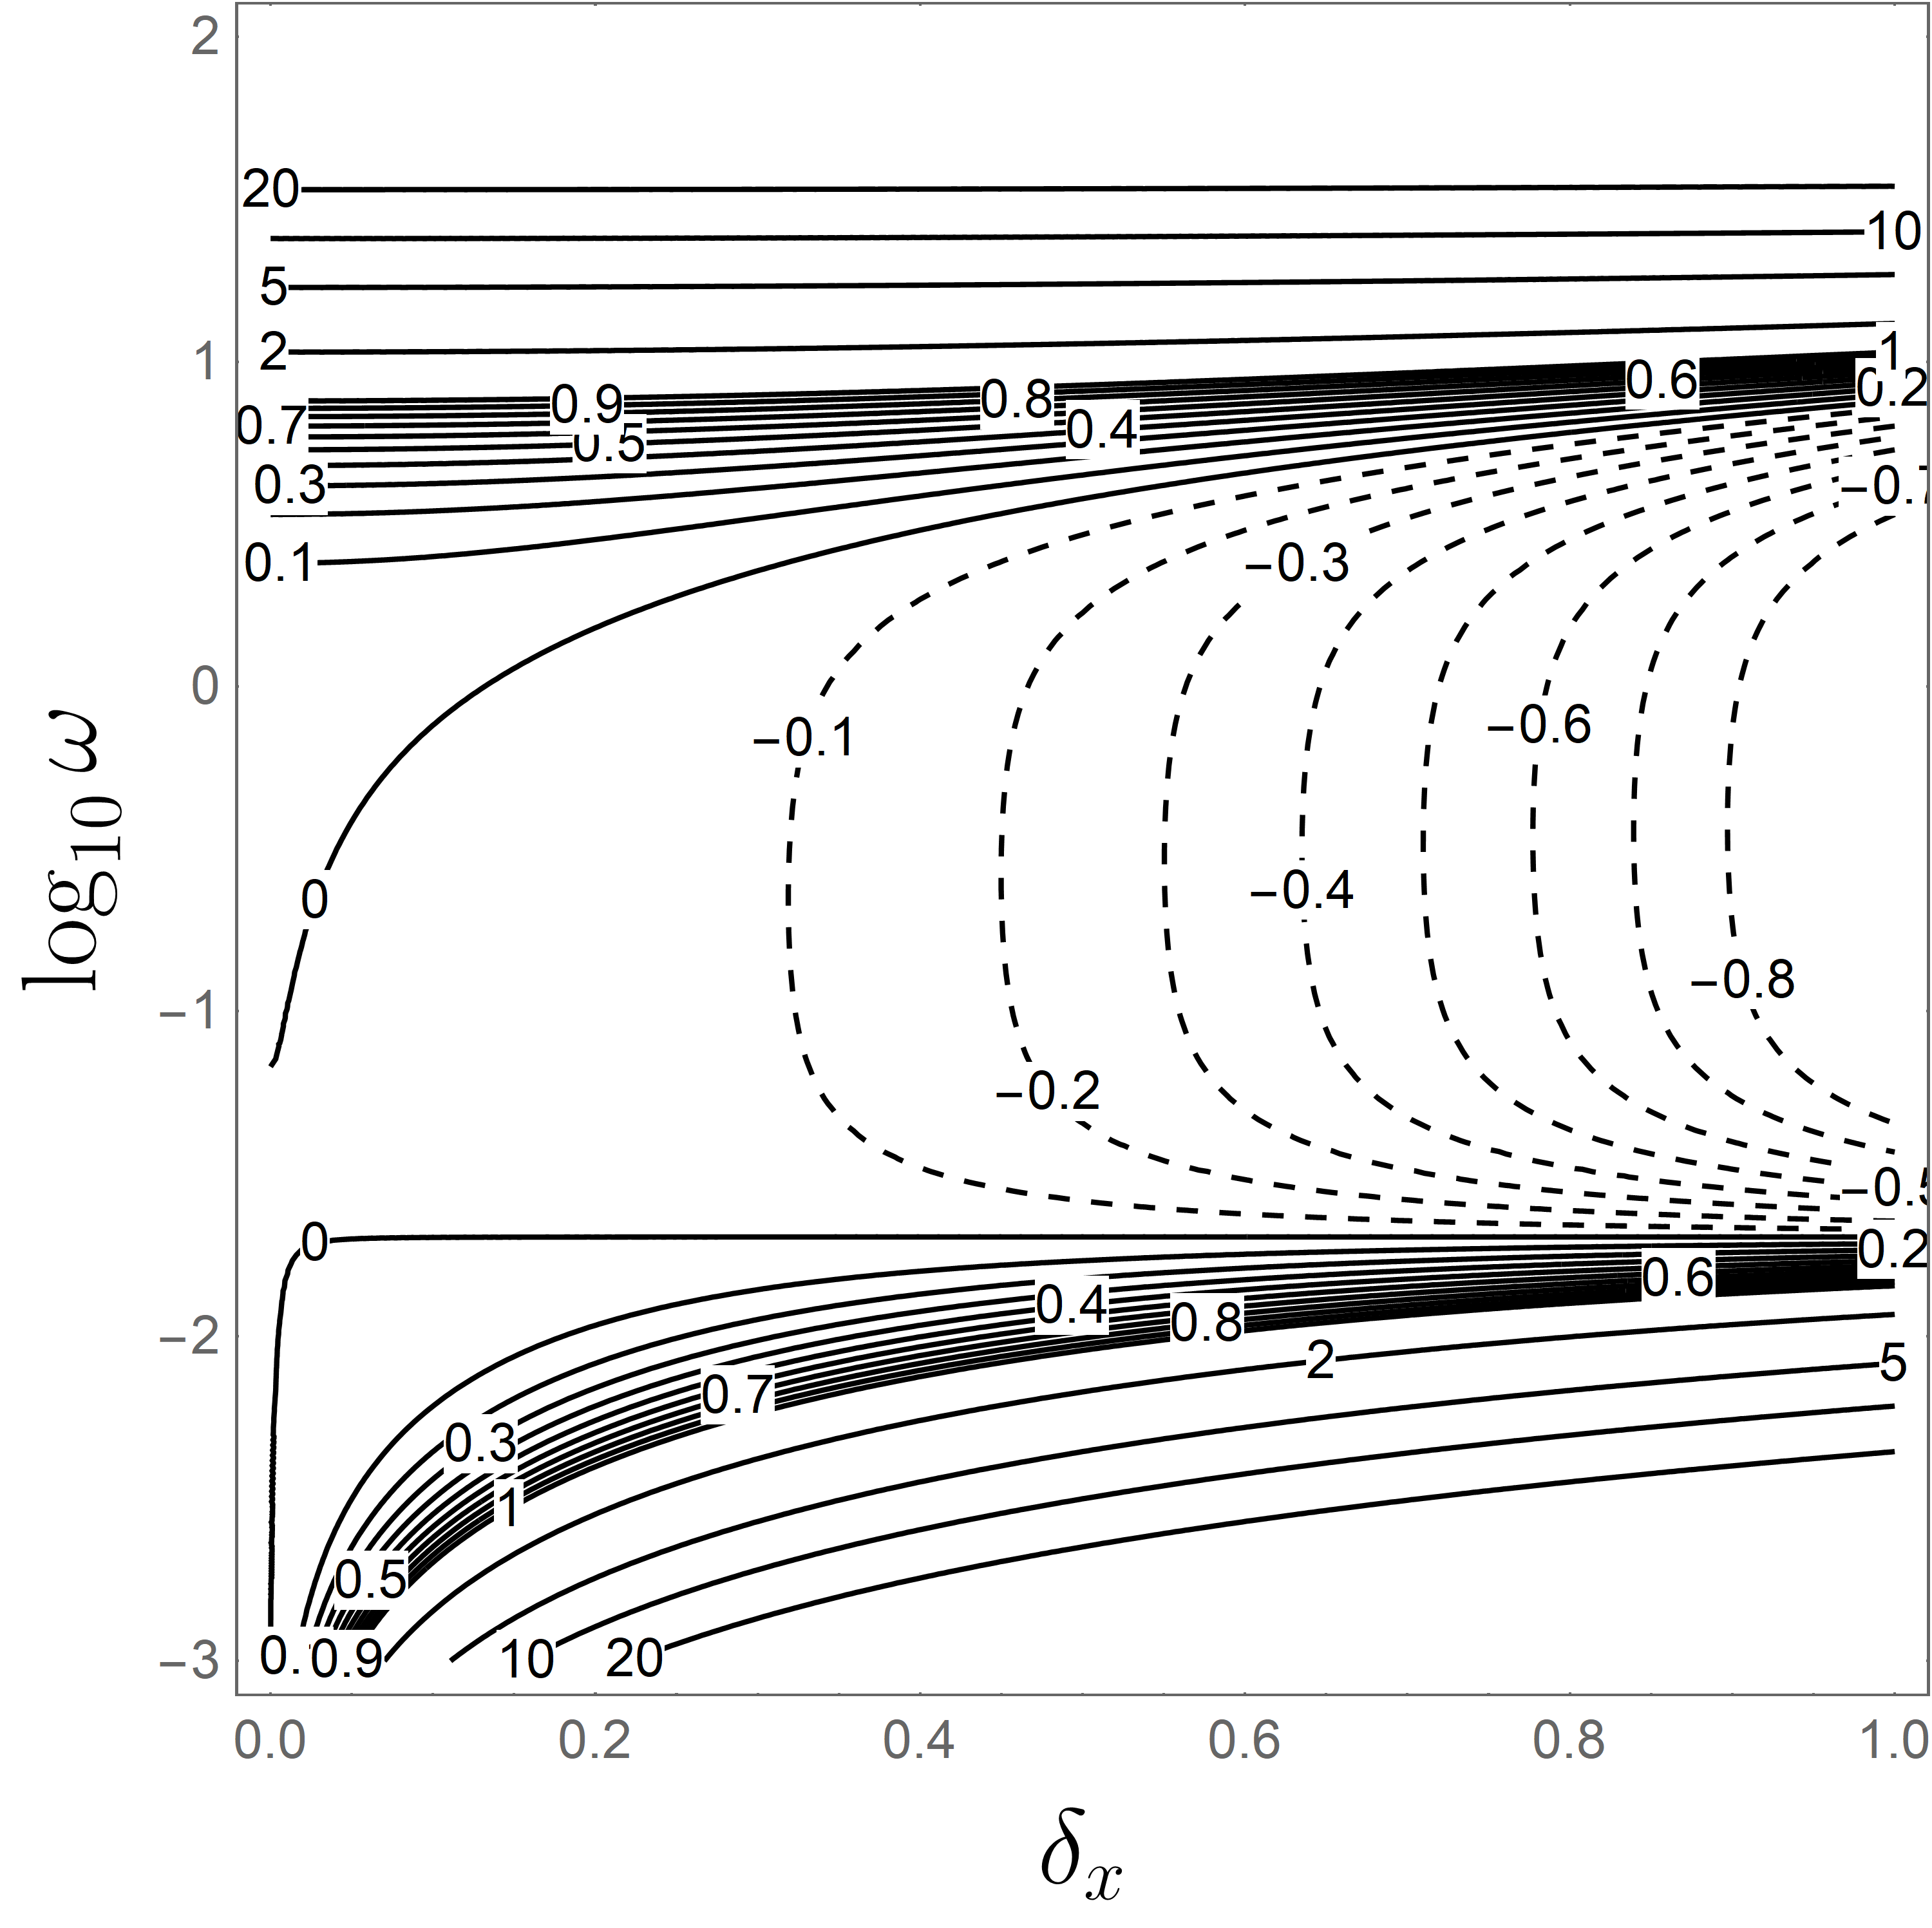
\includegraphics[width=0.5\linewidth]{FIGURES/Contour_dz.png}
	\caption{\textit{contours of $\ \delta_z^2(\delta_x,\ \omega)$}. Plain lines represent positive values $(\delta_z\in\mathbb{R})$, and dashed lines negative values $(\delta_z\in i\mathbb{R})$.}
	\label{FigContourdz}
\end{figure}
%
Figure \oldref{FigContourdz} shows variations of the squared vertical wavenumber $\delta_z^2$ as a function of $(\delta_x,\ \,\omega)$ for the values of $\epsilon_i, \epsilon_a$ given in table \ref{TableParameters}.  Negative values are encountered for medium-range frequencies $(10^{-1.7}<\omega<10^{0.7})$ and large enough horizontal wavenumbers $(\delta_x \geq 0.1-0.2)$. This region is surrounded by high and low frequency regions of positive $\delta_z^2$. The transition lines between these regions are given by $\delta_z=0$:
%
\begin{itemize}
	\item If $\omega \gg 1$ and $\epsilon_a \ne 0$ then $\omega^2\approx\omega_a^2$ and the transition line is given by 
	$\epsilon_a^2\omega^2 \approx
	\delta_x^2
 	+\frac{(\epsilon_a^2+\epsilon_i^2)^2}{4}$. This line is a parabola and the frequency is not bounded when $\delta_x$ increases. 
% 	When $\delta_x$ goes to 0, $\omega$ decreases monotically and reaches its lower bound for $\delta_x=0$: its minimum is given by $\omega_{c,a}=(\epsilon_a^2+\epsilon_i^2)/2\epsilon_a$.
	\item If $\omega \ll 1$ and $\epsilon_i \ne 0$ then $\omega^2\approx\omega_i^2$, the equation of the transition line is $\omega^2\approx\delta_x^2\epsilon_i^2/(\delta_x^2+(\epsilon_a^2+\epsilon_i^2)^2/4)$. This line has an upper bound $\omega_{c,i}=\epsilon_i$.
	In dimensional form, this bound can be rewritten $\Omega\leq N$ and is related to the well-known cut-off frequency for internal gravity waves.% \cite{dukowicz_2013}.
\end{itemize}
%
Therefore, the inner dispersion relation \ref{EqFullDispera} authorizes three types of wave solutions: two with real vertical wavenumbers $(\delta_z^2\geq0)$ and one with purely imaginary wavenumbers $(\delta_z^2<0)$.

\subsubsection{Real vertical wavenumber $(\delta_z\in\mathbb{R})$}
\label{realwavenumber}
%Figure \ref{FigContourdz} presents the evolution of the square of the vertical wave-number as a function of $\delta_x$ and $\omega$. Two regions of positive $(\delta_z^2)$ are separated by one region of negative $(\delta_z^2)$. 

The ratio of reference functions $\displaystyle R^2(\delta_x,\delta_z)$, defined by \ref{eqratio}, depends on two variables $(\delta_x,\ \delta_z)$ and two parameters $(\epsilon_i,\ \epsilon_a)$. A study of its variations for $\delta_x \in \mathbb{R}$ shows that, for non-vanishing $(\epsilon_i,\ \epsilon_a)$, it has an upper bound:
%
\begin{equation}
	 \max_{\delta_x} R^2(\delta_x,\delta_z) =\frac{1}{4}
	\frac{\epsilon_a^2\epsilon_i^2}{\delta_z^2+\frac{\left
	(\epsilon_a^2+\epsilon_i^2
	\right)^2}{4}}.
\label{boundR2}
\end{equation}
%
This maximum value is attained for $\delta_x^2=\delta_z^2+\frac{(\epsilon_a^2+\epsilon_i^2)^2}{4}$.
We see that $R^2$ approaches $1/4$ (and thus the two roots $\omega_+$ and $\omega_-$ coincide) for both a near depth-independent vertical profile (i.e. $\delta_z \approx 0$\footnote{We use the term {\it depth-independent} even if $F(z)$ is a linear function of $z$ when $\delta_z$ is close to $0$ (see \ref{EqDispRef}), so that the vertical profile of $W(z)$ is approximately linear while the vertical profile of $U(z)$ is approximately constant.}) and $\epsilon_a \approx \epsilon_i$ (or in dimensional form $N=g/c_s$). This last equality is true when the stratification and the compressibility effects have an identical contribution to the vertical variation of background stratification $\hat{\rho}_h(z)$. In all other cases, the vast majority, the two roots are well separated and given by:
%Since we are here in the case of an unbounded ocean\footnote{If this constraint would have been omitted, a value of $R^2=\frac{1}{4}$ could be attained for $\delta_z=0$, $\epsilon_i=\epsilon_a$. In this case, $\delta_x^2=\frac{(\epsilon_a^2+\epsilon_i^2)^2}{4}=\epsilon_a^4$ and this leads to a dual root of $\omega_\pm^2=\frac{\omega_a^2}{2}=\frac{\delta_x^2}{\epsilon_a^2}=\epsilon_a^2$ (or $\Omega^2=c_s^2k_x^2$).}, we do not consider the case of small $\delta_z$ and  \ref{boundR2} shows that  $R$ is small and thus the two solutions are well separated with 
\begin{equation}
\omega_{-}(\delta_x,\ \delta_z) \approx \omega_i
(\delta_x,\ \delta_z), \quad
\omega_{+}(\delta_x,\ \delta_z) \approx \omega_a(\delta_x,\ \delta_z)
\end{equation}
These two roots are studied below.

\paragraph{Modified internal waves (MIW)}
The traditional dispersion relation for dispersive internal gravity wave rays in the context of a Boussinesq incompressible fluid (\citealt{gill_1982}; see also Table \oldref{TableWave solutions} above) is:
%
\begin{equation}
\omega_{iwr}^2=\epsilon_i^2\frac{ \delta_x^2}{\delta_x^2+\delta_z^2}
\label{DispRays}
\end{equation}
%
A Taylor expansion of the gravity-wave root $\omega_{-}^2$ given by \ref{solseq} with respect to the small parameters $\epsilon_a$ and $\epsilon_i$ leads to:
\begin{align}
\frac{\omega_-^2}{\omega_{iwr}^2}&=1
-
	\left(
	\frac{(\epsilon_i^2+\epsilon_a^2)^2}{4(\delta_x^2+\delta_z^2)}
	-\frac{\epsilon_i^2\epsilon_a^2 \delta_x^2}{(\delta_x^2+\delta_z^2)^2}
	\right)
+\mathrm{O}((\epsilon_i^{2}+\epsilon_a^{2})^4) \label{DispRaysDT}
\\
&=1
-\underbrace{\frac{(\epsilon_i^2+\epsilon_a^2)^2\delta_z^2+(\epsilon_a^2-\epsilon_i^2)^2\delta_x^2}{4(\delta_x^2+\delta_z^2)^2}}_{\mathrm{O}((\epsilon_i^{2}+\epsilon_a^{2})^2)}
+\mathrm{O}((\epsilon_i^{2}+\epsilon_a^{2})^4),  \label{DispRaysDTfact}
\end{align}
%
while the development of $\omega_i^2$ leads to
\[
\frac{\omega_i^2}{\omega_{iwr}^2}=1
-\underbrace{\frac{(\epsilon_i^2+\epsilon_a^2)^2}{4(\delta_x^2+\delta_z^2)}}_{\mathrm{O}((\epsilon_i^{2}+\epsilon_a^{2})^2)}
+\mathrm{O}((\epsilon_i^{2}+\epsilon_a^{2})^4).
\]
Compared with $\omega_i^2$, $\omega_-^2$ includes corrective terms due to the two roots of the inner dispersion relation not being fully separated. The corrective term $\displaystyle \frac{\epsilon_i^2\epsilon_a^2 \delta_x^2}{4(\delta_x^2+\delta_z^2)^2}$ is naturally close to $R^2$. It is trivial to see from formulation \ref{DispRaysDTfact} that the combined effect of compressibility and stratification is always a reduction of frequency, compared with the approximated value $\omega_{iwr}$: $\omega_-^2\le \omega_{iwr}^2$.\\
%is recovered at fourth order in $\epsilon_i$ and $\epsilon_a$.
%Relations \ref{DispRaysDT} and \ref{DispRays} further show that $\omega_{iwr}^2/\epsilon_i^2$ is a fourth-order approximation of $\omega_i^2/\epsilon_i^2$ and is itself an approximation of the general root $\omega_-^2/\epsilon_i^2$.
%As a consequence, when parameters $\epsilon_i^2$ and $\epsilon_a^2$  are both small, the stratification function $\omega_i(\delta_x,\delta_z)$ is an internal gravity wave ray modified by compressibility and propagating in an unbounded ocean.
%%Both corrective terms on the right-hand-side are proportional to $\epsilon_i^2+\epsilon_a^2=H/D_0$ and consequently depends on the relative strength of the stratification (with no compressibility correction).
%The first corrective term can only reduce the pulsation, the last term can only increase it. However it can be shown that the combined effect is always a reduction of the pulsation, i.e. $\omega_{-}^2 \le \omega_{iwr}^2$. We postpone the discussion on the compressibilty effects on the pulsation in the section on bounded ocean. Indeed, as can be seen on Eq. \ref{DispRaysDT} this effect is strongly dependent on the vertical wavenumber $\delta_z$ whose possible values are limited in the bounded ocean cases.\\

Ocean waves satisfying \ref{DispRaysDT} will now be referred to as \textit{Modified Internal Waves (MIW)}.
\\

{\color{red}AJOUTER PLOTS DE $\omega_-^2/\omega_{iwr}^2$ pour differentes valeurs de epsi, epsa}

\paragraph{Modified acoustic waves (MAW)}
The well-known dispersion relation for acoustic waves in an homogeneous fluid is:
%
\begin{equation}
\omega_{aw}^2 =\frac{1}{\epsilon_a^2}\left(\delta_x^2+\delta_z^2\right)
\label{DispAcous}
\end{equation}
%
A Taylor development of the acoustic root $(\omega_+)$ with respect to $\epsilon_a$ and $\epsilon_i$ leads this time to:
%
\begin{align}
\frac{\omega_+^2}{\omega_{aw}^2}&=1
+
\left(
\frac{(\epsilon_i^2+\epsilon_a^2)^2}{4(\delta_x^2+\delta_z^2)}
-\frac{\epsilon_i^2\epsilon_a^2 \delta_x^2}{(\delta_x^2+\delta_z^2)^2}
\right)
+\mathrm{O}((\epsilon_i^{2}+\epsilon_a^{2})^4)
\label{DispAcousDT}\\
&=1+\underbrace{\frac{(\epsilon_i^2+\epsilon_a^2)^2\delta_z^2+(\epsilon_a^2-\epsilon_i^2)^2\delta_x^2}{4(\delta_x^2+\delta_z^2)^2}}_{\mathrm{O}((\epsilon_i^{2}+\epsilon_a^{2})^2)}
+\mathrm{O}((\epsilon_i^{2}+\epsilon_a^{2})^4), \label{DispAcousDTfact}
\end{align}
%
while the development of $\omega_a^2$ leads to
\[
\frac{\omega_a^2}{\omega_{aw}^2}=1+
\underbrace{\frac{(\epsilon_i^2+\epsilon_a^2)^2}{4(\delta_x^2+\delta_z^2)}}_{\mathrm{O}((\epsilon_i^{2}+\epsilon_a^{2})^2)}
+\mathrm{O}((\epsilon_i^{2}+\epsilon_a^{2})^4).
\]
Compared with $\omega_a^2$, $\omega_+^2$ includes corrective terms due to the two roots of the inner dispersion relation not being fully separated. Again, the corrective term is small and close to $R^2$. The combined effect of compressibility and stratification is always an increase of frequency, compared with the approximated value $\omega_{aw}$: $\omega_+^2\ge \omega_{aw}^2$.\\

Ocean waves satisfying \ref{DispAcousDT} will be called \textit{Modified Acoustic Waves (MAW)} in the following. The modifications to usual internal and acoustic wave dispersion relations by compressibility and stratification effects are expressed by:
\[
\omega_+^2\omega_-^2=\frac{\epsilon_i^2}{\epsilon_a^2}\delta_x^2=\omega_{aw}^2\omega_{iwr}^2,
\]
which explains the symmetry in the above developments for modified internal and acoustic waves.
{\color{red}AJOUTER PLOTS DE $\omega_+^2/\omega_{aw}^2$ pour differentes valeus de epsi, epsa}

\subsubsection{Purely imaginary vertical wavenumber $(\delta_z\in i\ 
\mathbb{R})$}
\label{subsubsectioniR}

If now $\delta_z$ is a purely imaginary complex, it can be written $\delta_z=i\delta_{z,i}$ with $\delta_{z,i}\in\mathbb{R}$ and wave solutions are vertically evanescent. The boundary dispersion relation now writes:
\begin{equation}
\label{EqFullDisperbi}
\omega^2=\frac{\delta_x^2\tanh(\delta_{z,i})}
{\delta_{z,i}+\frac{\epsilon_a^2+\epsilon_i^2}{2}\tanh(\delta_{z,i})}
\end{equation}
and the inner dispersion relation:
%
\begin{equation}
	\label{EqFullDisperai}
 		\delta_x^2-\delta_{z,i}^2 =\epsilon_i^2\frac{\delta_x^2}
 			{\omega^2}+\epsilon_a^2\omega^2-\frac{(\epsilon_a^2+\epsilon_i^2)^2}{4}
		%\label{EqFullDisperbi}
		%& \omega^2 &&=\frac{\delta_x^2\ tanh(\delta_{z,i})}
		%{\delta_{z,i}+\frac{\epsilon_a^2+\epsilon_i^2}			{2}tanh(\delta_{z,i})}
		%=\frac{\delta_x^2}{\frac{\epsilon_a^2+\epsilon_i^2}{2}
		%+\delta_z cotan(\delta_z)}
\end{equation}
%
When horizontal and vertical wavenumbers are close together, the left-hand side and  right-hand side of  \ref{EqFullDisperai} both vanish, i.e., the influence of stratification $(\epsilon_i^2\delta_x^2/\omega^2)$ and compressibility $(\epsilon_a^2\omega_a^2)$ cancel out. In other words, differences between horizontal and vertical wavenumbers are indication of the influence of ocean stratification and/or compressibility. In an incompressible, homogeneous (unstratified) ocean, $\epsilon_i=\epsilon_a=0$ and vertical and horizontal wave-numbers are equal.

The developments of $\omega_-^2, \omega_+^2$ for small $\epsilon_i, \epsilon_a$ are identical to those for real vertical wavenumbers \ref{DispRaysDT}, \ref{DispAcousDT} just replacing $\delta_z^2$ by $-\delta_{z,i}^2$.

The remaining question is that of root separation when $\delta_z\in i\ \mathbb{R}$. Unlike when $\delta_z\in \mathbb{R}$ (previous sub-section), the ratio $R^2(\delta_x,\ i\ \delta_{z,i})$ can be equal to $1/4$ even when $\delta_z$ is not small.
Relation \ref{EqFullDisperai} imposes $0\le \delta_{z,i}^2\le \delta_x^2+\frac{(\epsilon_a^2+\epsilon_i^2)^2}{4}$ and in this range of values, $R^2$ is an increasing function of $\delta_{z,i}^2$. The value of $R^2=1/4$ is attained for $\delta_{z,i}^2=\delta_{z,i,\star}^2$ given by:
%
\begin{equation}
	\delta_{z,i,\star}^2=\delta_x^2+\frac{(\epsilon_a^2+\epsilon_i^2)^2}{4}-2\epsilon_a\epsilon_i\delta_x,
	\label{deltazi}
\end{equation} 
%
for which the inner dispersion relation has a double root $\displaystyle \omega_+^2 = \omega_-^2 = \frac{\epsilon_i}{\epsilon_a}\delta_x$.
When $\delta_{z,i}$ is less than $\delta_{z,i,\star}$, the two roots become separated.
Again, since we look only at regular solutions, the case $\delta_{z,i}^2>\delta_{z,i,\star}^2$, which would lead to $R^2 > 1/4$ is not considered.

Even if \ref{EqFullDisperai} has two roots, the two corresponding branches are always connected, as shown above, and thus form one family of ocean waves.
Ocean waves satisfying \ref{EqFullDisperai} will be called {\it Modified Surface Waves (MSW)} in the following.
%Far from this region, i.e. if can find a strictly-positive constant $\alpha$ such that:
%%i.e. if we can find $\alpha>0$ such that $R^2\leq 1/4(1-\alpha^2)$ or in $(\delta_x,\ \delta_z,\ \omega)$ phase-space (sufficient relation):
%\begin{equation}
%	\label{regsepi}
%	\delta_x^2-\delta_{z,i}^2\geq
%	\frac{2\epsilon_i\epsilon_a\delta_x}
%	{\sqrt{1-\alpha^2}}
%\end{equation}
%then, from Relation \ref{eqratio}, $R^2\leq (1-\alpha^2)/4$ and, from Relation \ref{deltaomegapm}, the roots are well-separated:
%\begin{subequations}
%	\begin{alignat}{2}	
%	&\omega_{+}^2-\omega_{-}^2 &&=\omega_a^2\sqrt{1-4 R^2}\\[3mm]
%	& &&\geq \alpha\omega_a^2 
%	\geq \alpha\frac{(\epsilon_i^2+\epsilon_a^2)^2}{4\epsilon_a^2}
%	\end{alignat}
%\end{subequations}
%Then the relations \ref{Comp1} and \ref{Comp2} with \ref{regsepi} lead to two additional inequalities:
%\begin{subequations}
%	\begin{alignat}{2}
%	\label{Comp1b}
%	&\omega_a^2(\delta_x,\ i\delta_{z,i})-\omega_{+}^2(\delta_x,\ i\delta_{z,i})
%	&&\leq\frac{\epsilon_i\sqrt{1-\alpha^2}}{2\epsilon_a}\ \delta_x\\[3mm]
%	\label{Comp2b}
%	&\omega_{-}^2(\delta_x,\ i\delta_{z,i})-\omega_i^2(\delta_x,\ i\delta_{z,i})
%	&& \leq\frac{\epsilon_i (1-\alpha^2)^{3/2}}{2\epsilon_a}\frac{1}{\delta_x}
%	\end{alignat}	
%\end{subequations}
%These relations show that for $\delta_z\in i\ \mathbb{R}$, the roots are well-separated in the region of phase-space far enough from the plane $\delta_x=\delta_{z,i}$ \ref{regsepi}.
% and, in such a region of the phase space, the root $\omega_+$ (respectively $\omega_-$) can be as close as required from the acoustic (stratification) function if $\delta_x$ is decreased (respectively increased).


%\ref{EqFullDisper} has indeed a double ro
%If $\delta_z\in i\ \mathbb{R}$, \ref{EqFullDisperai} does not necessarily have two real %roots. Indeed it can vanish for $R^2=1/4$ or



%\begin{figure}[!h]
%	\centering		
%	\begin{subfigure}{0.45\linewidth}
%		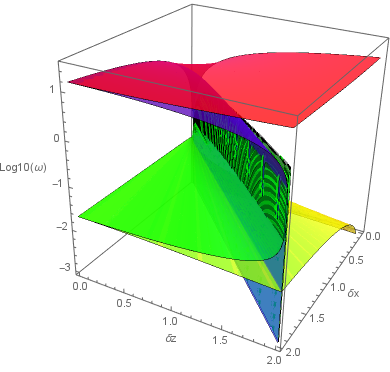
\includegraphics[width=1\linewidth]{FIGURES/Fig_omega.png}
%		\caption{}
%	\end{subfigure}
%	~
%	\centering		
%	\begin{subfigure}{0.45\linewidth}
%		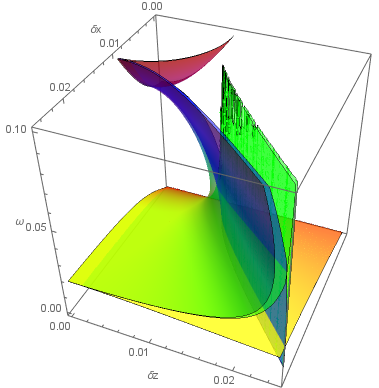
\includegraphics[width=1\linewidth]{FIGURES/Fig_omega_zoom.png}
%		\caption{}
%	\end{subfigure}
%	~
%	\caption{\textit{inner dispersion surface and factorizing functions $\omega_a$ and $\omega_i$. Polychrome: inner dispersion surface. Red: $\omega^2=\omega_a^2(\delta_x,\ \delta_z)$. Blue: : $\omega^2=\omega_a^2(\delta_x,\ i \delta_z)$. Green: $\omega^2=\omega_i^2(\delta_x,\ i \delta_z)$. Yellow: $\omega^2=\omega_i^2(\delta_x,\ \delta_z)$. (b) is a zoom of (a) in the vicinity of the origin.}}
%	\label{FigOmega}
%\end{figure}

\subsection{Summary: waves solutions in an unbounded ocean}
\label{SubSectionUsualDisp}

In the preceding analysis, three types of waves were identified. A synthesis is given by Figure \oldref{FigFullstratifiedcompressible} showing the inner dispersion surfaces for a stratified compressible ocean, and Figure \oldref{FigFullsimplifiedcases} showing limit cases for a homogeneous incompressible ocean. The values of the parameters $\epsilon_a, \epsilon_i$ are those of Table \oldref{TableParameters}.
%
\begin{figure}[h]
	\centerline{
		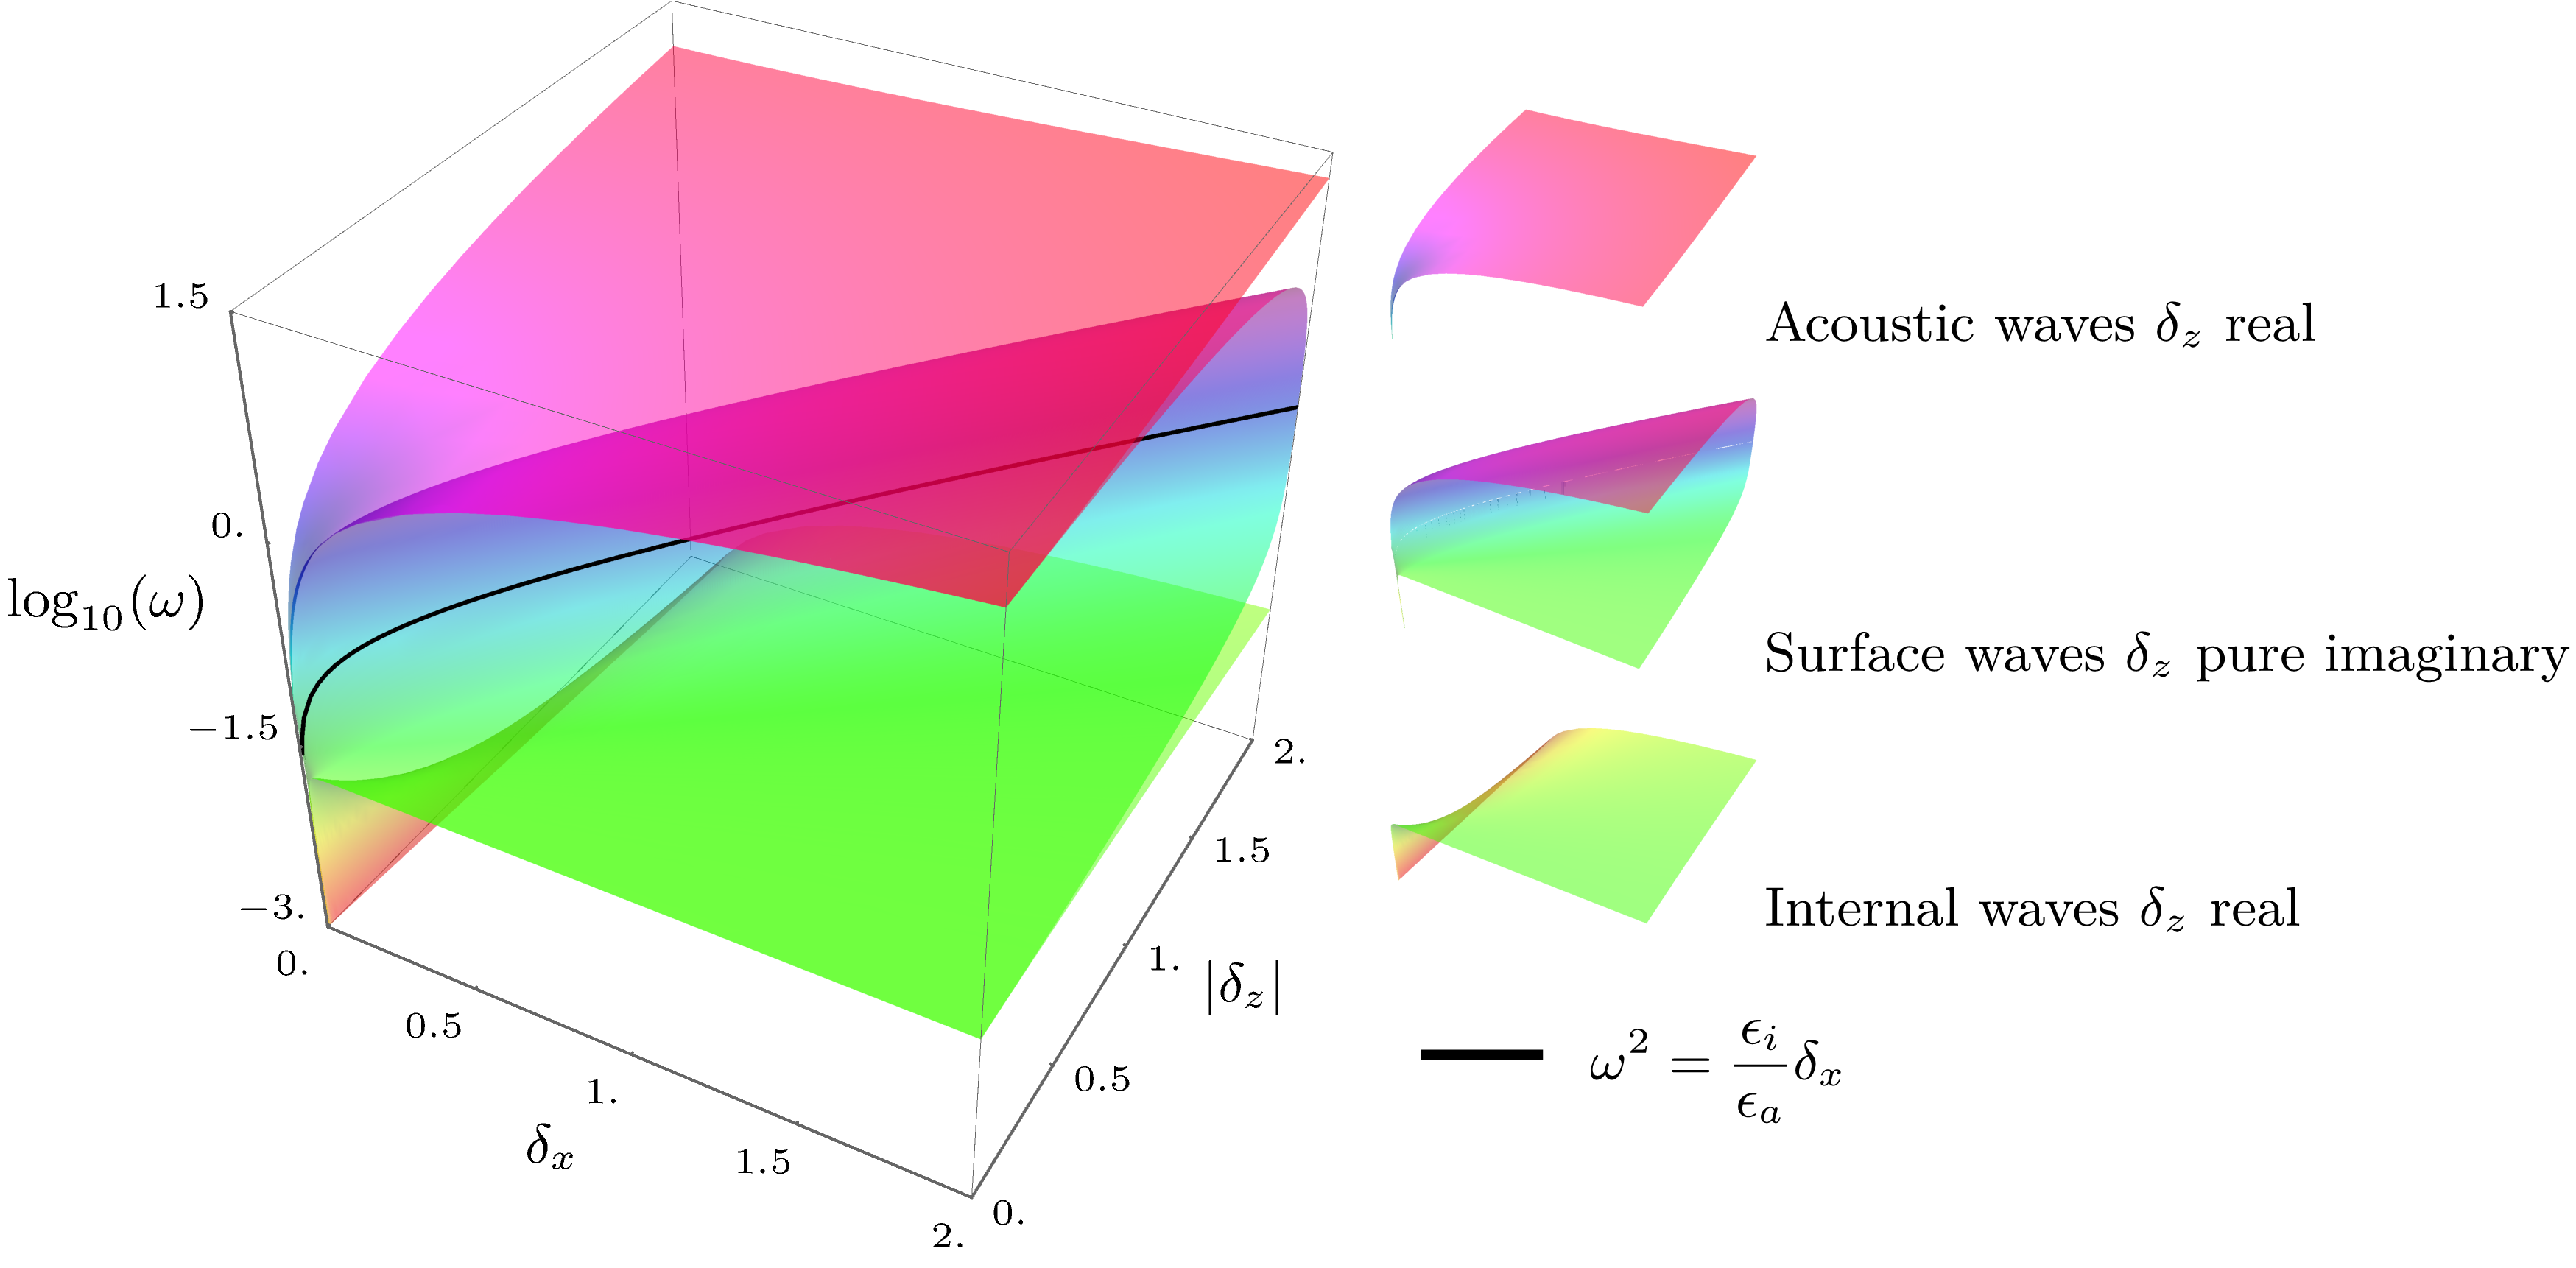
\includegraphics[width=1\linewidth]{FIGURES/unboundedwaves.png}
	}
	\caption{Inner dispersion surfaces in $(\delta_x, \delta_z, \log_{10}(\omega))$ space for a stratified and compressible ocean. The surfaces are colored by the magnitude of frequency $\omega$.}
	\label{FigFullstratifiedcompressible}
\end{figure}
\\
\begin{figure}[h]
	\centering		
	%\begin{subfigure}{0.45\linewidth}
	\subfloat[][$\epsilon_a=0$]{
		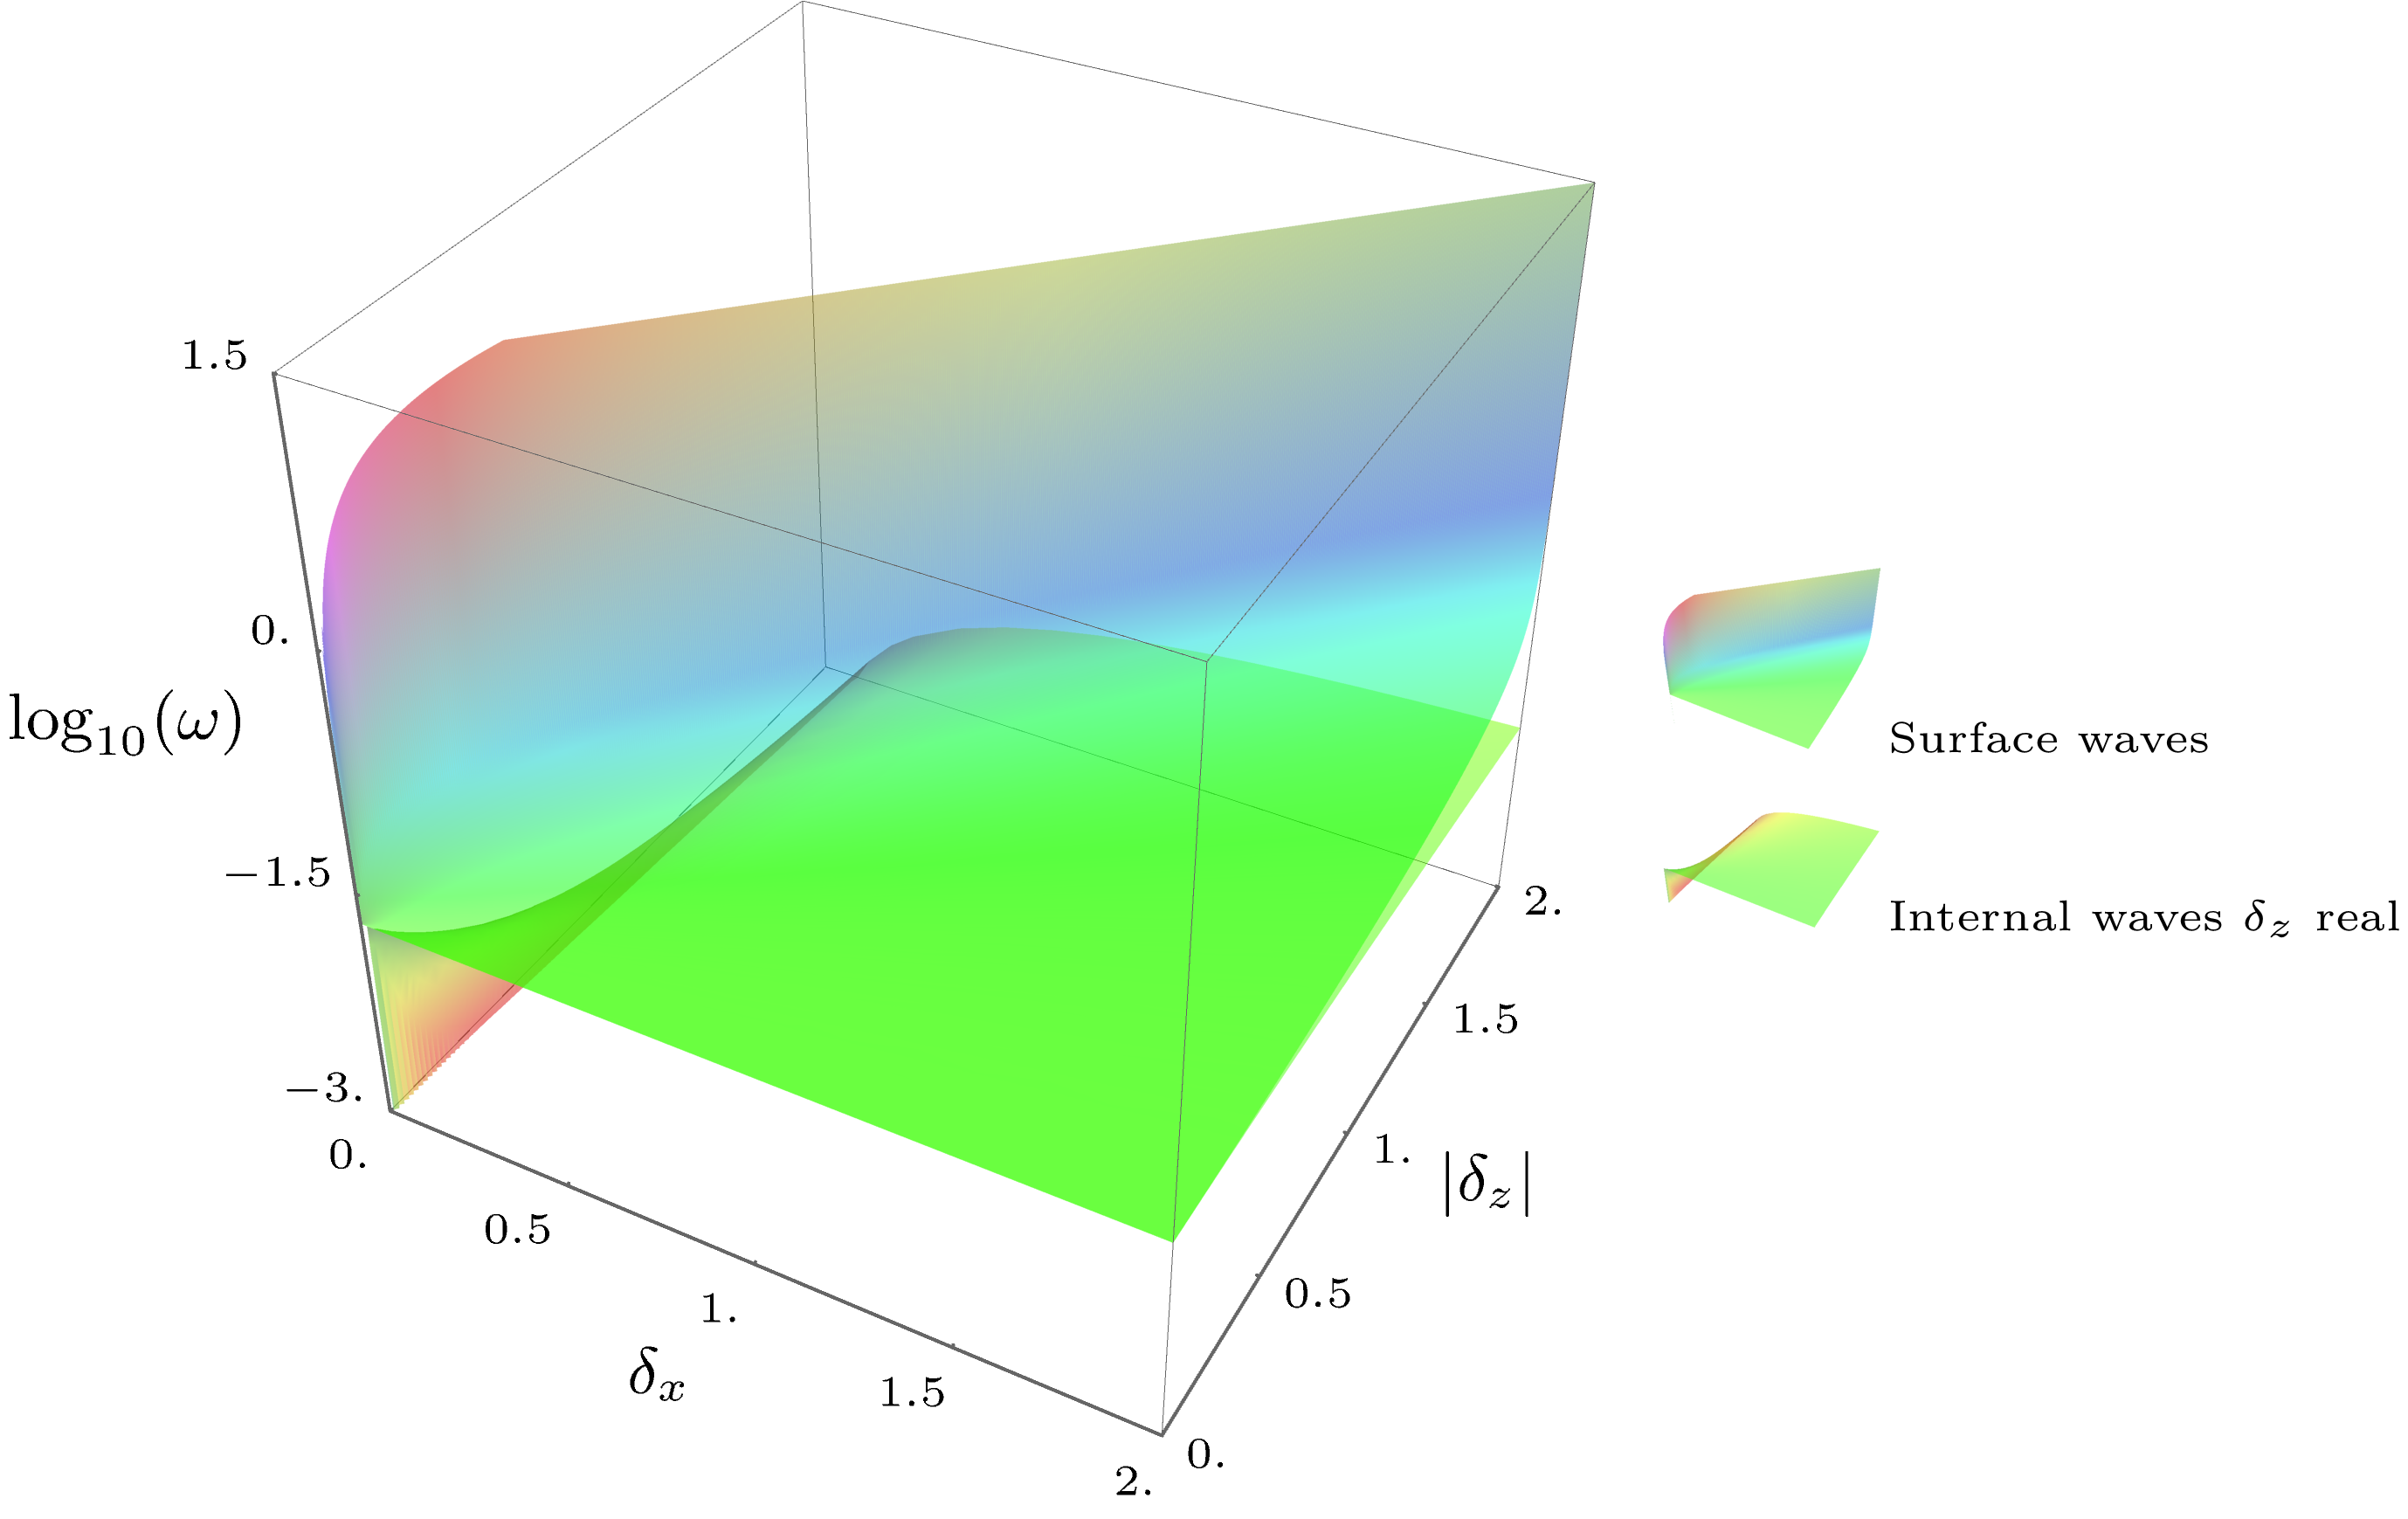
\includegraphics[width=0.35\linewidth]{FIGURES/unboundedwavesepsa0.png}
	}	
	\subfloat[][$\epsilon_i=0$]{
		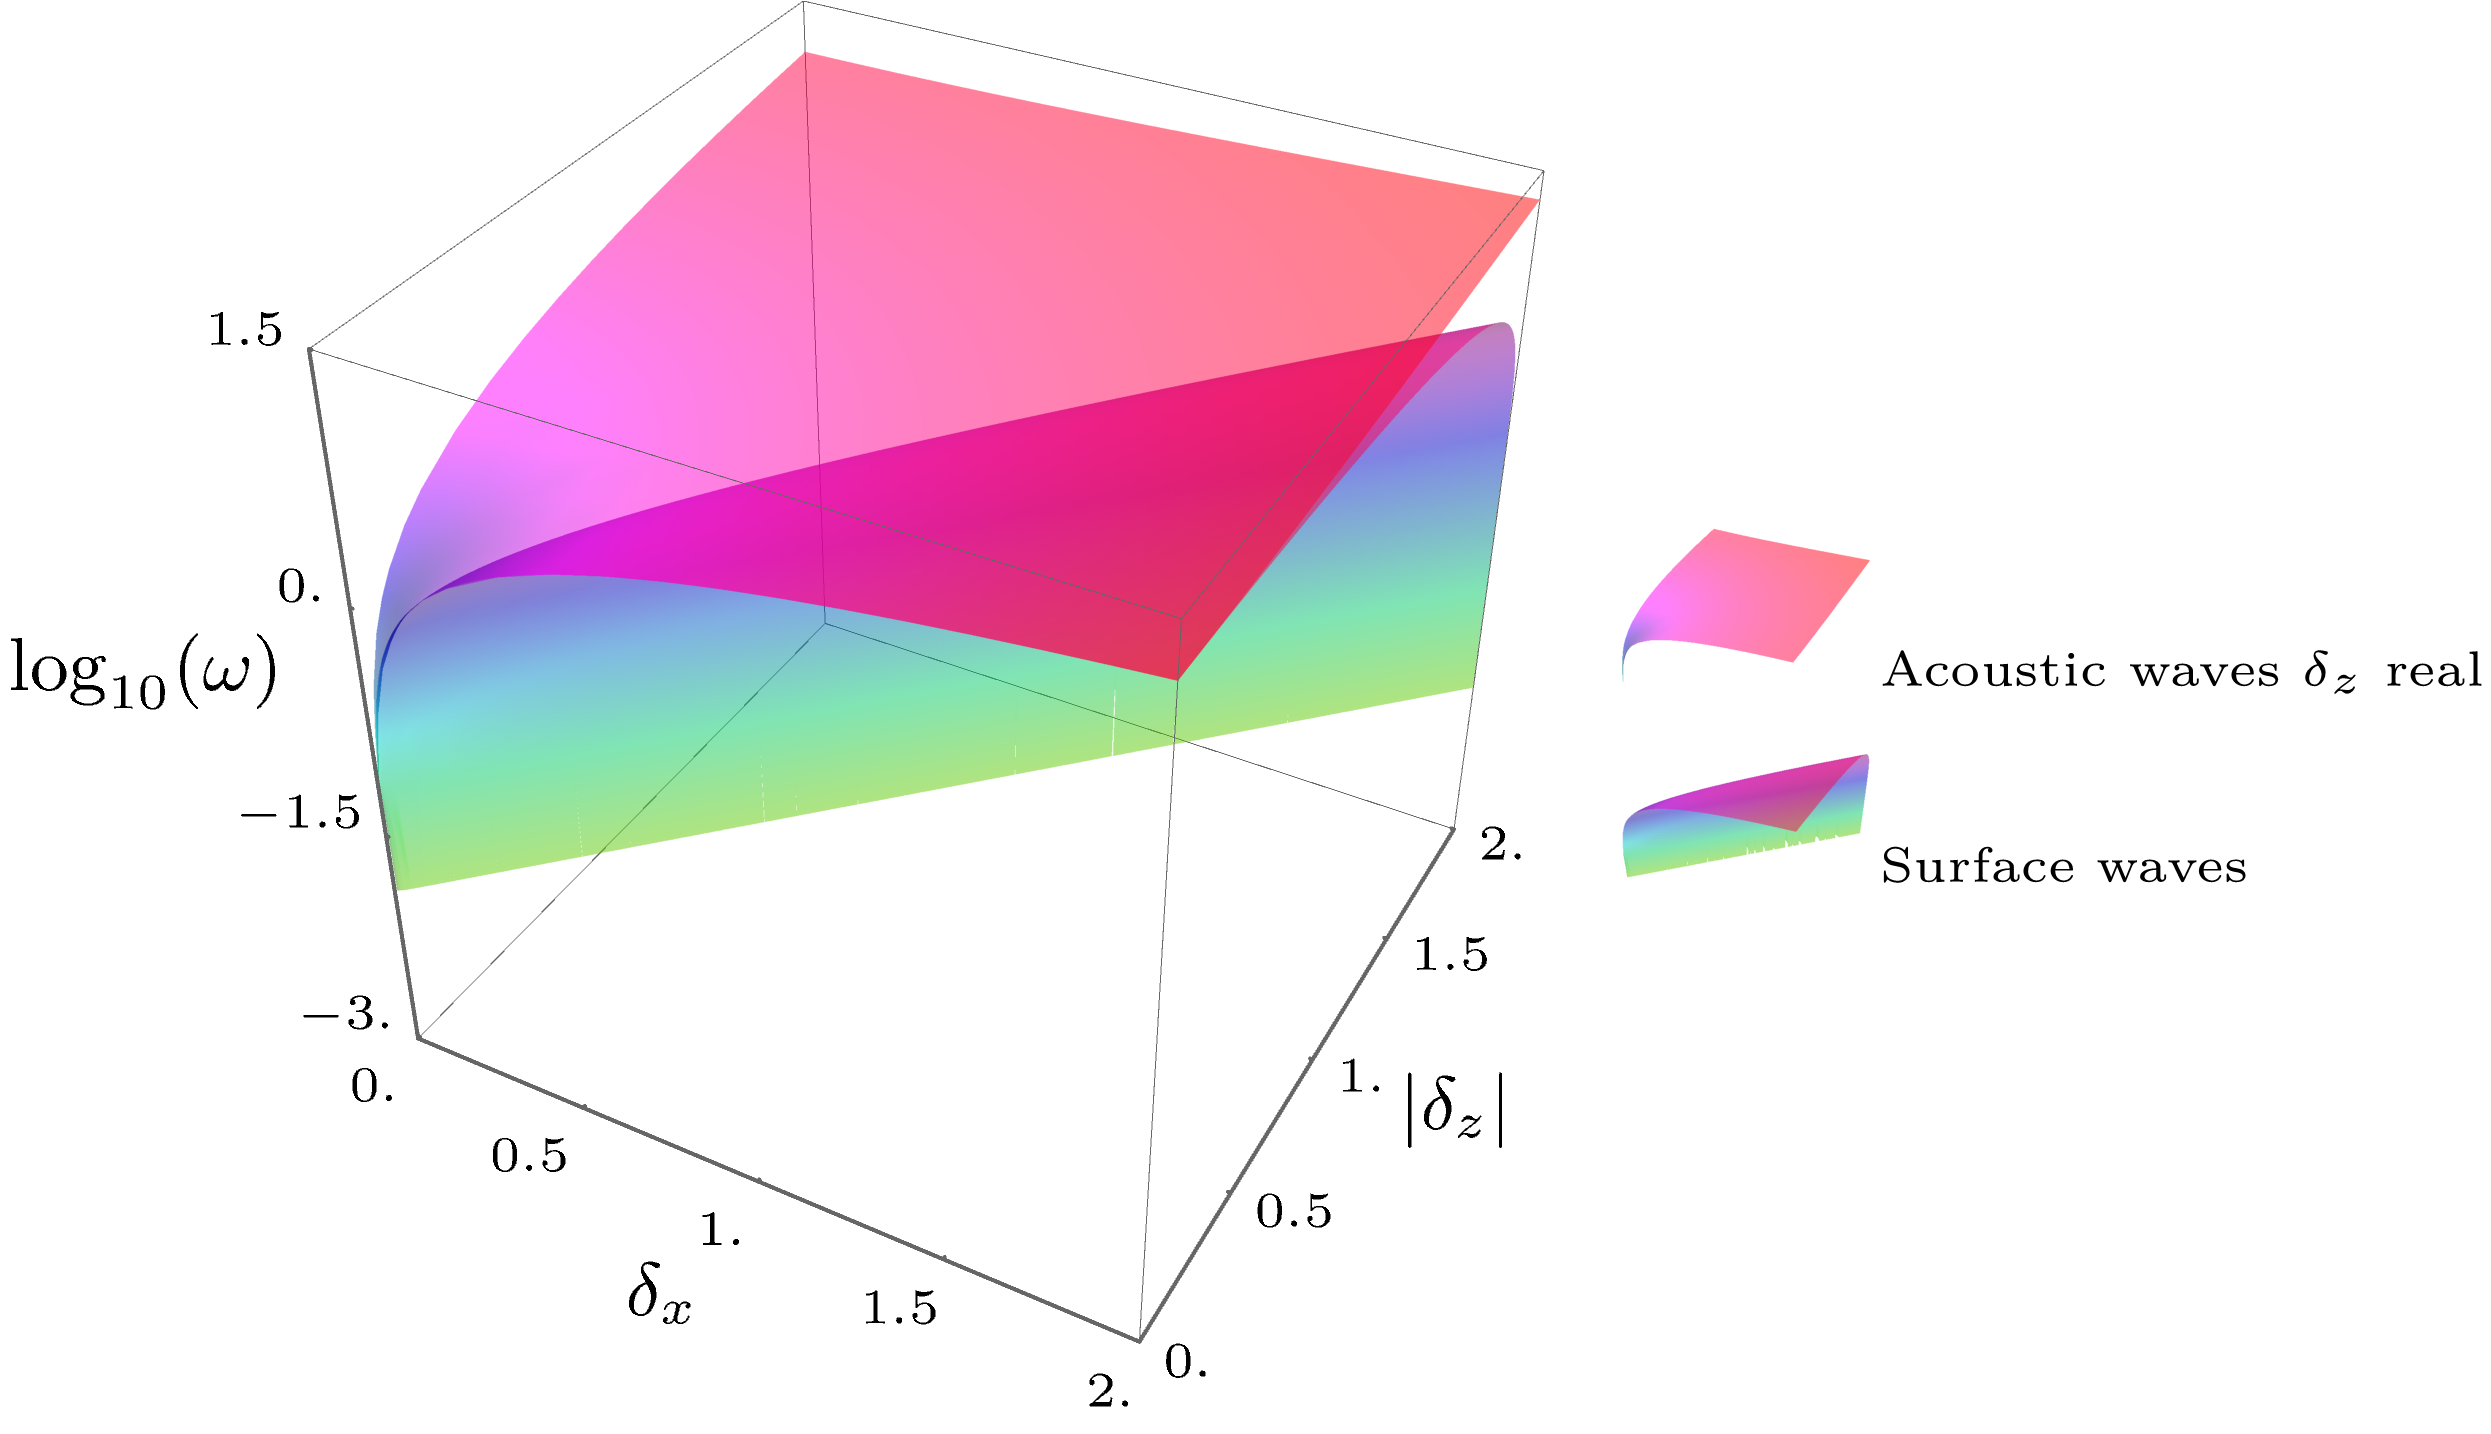
\includegraphics[width=0.35\linewidth]{FIGURES/unboundedwavesepsi0.png}
	}
	\\
	\centering		
	\subfloat[][$\epsilon_a=\epsilon_i=0$]{
		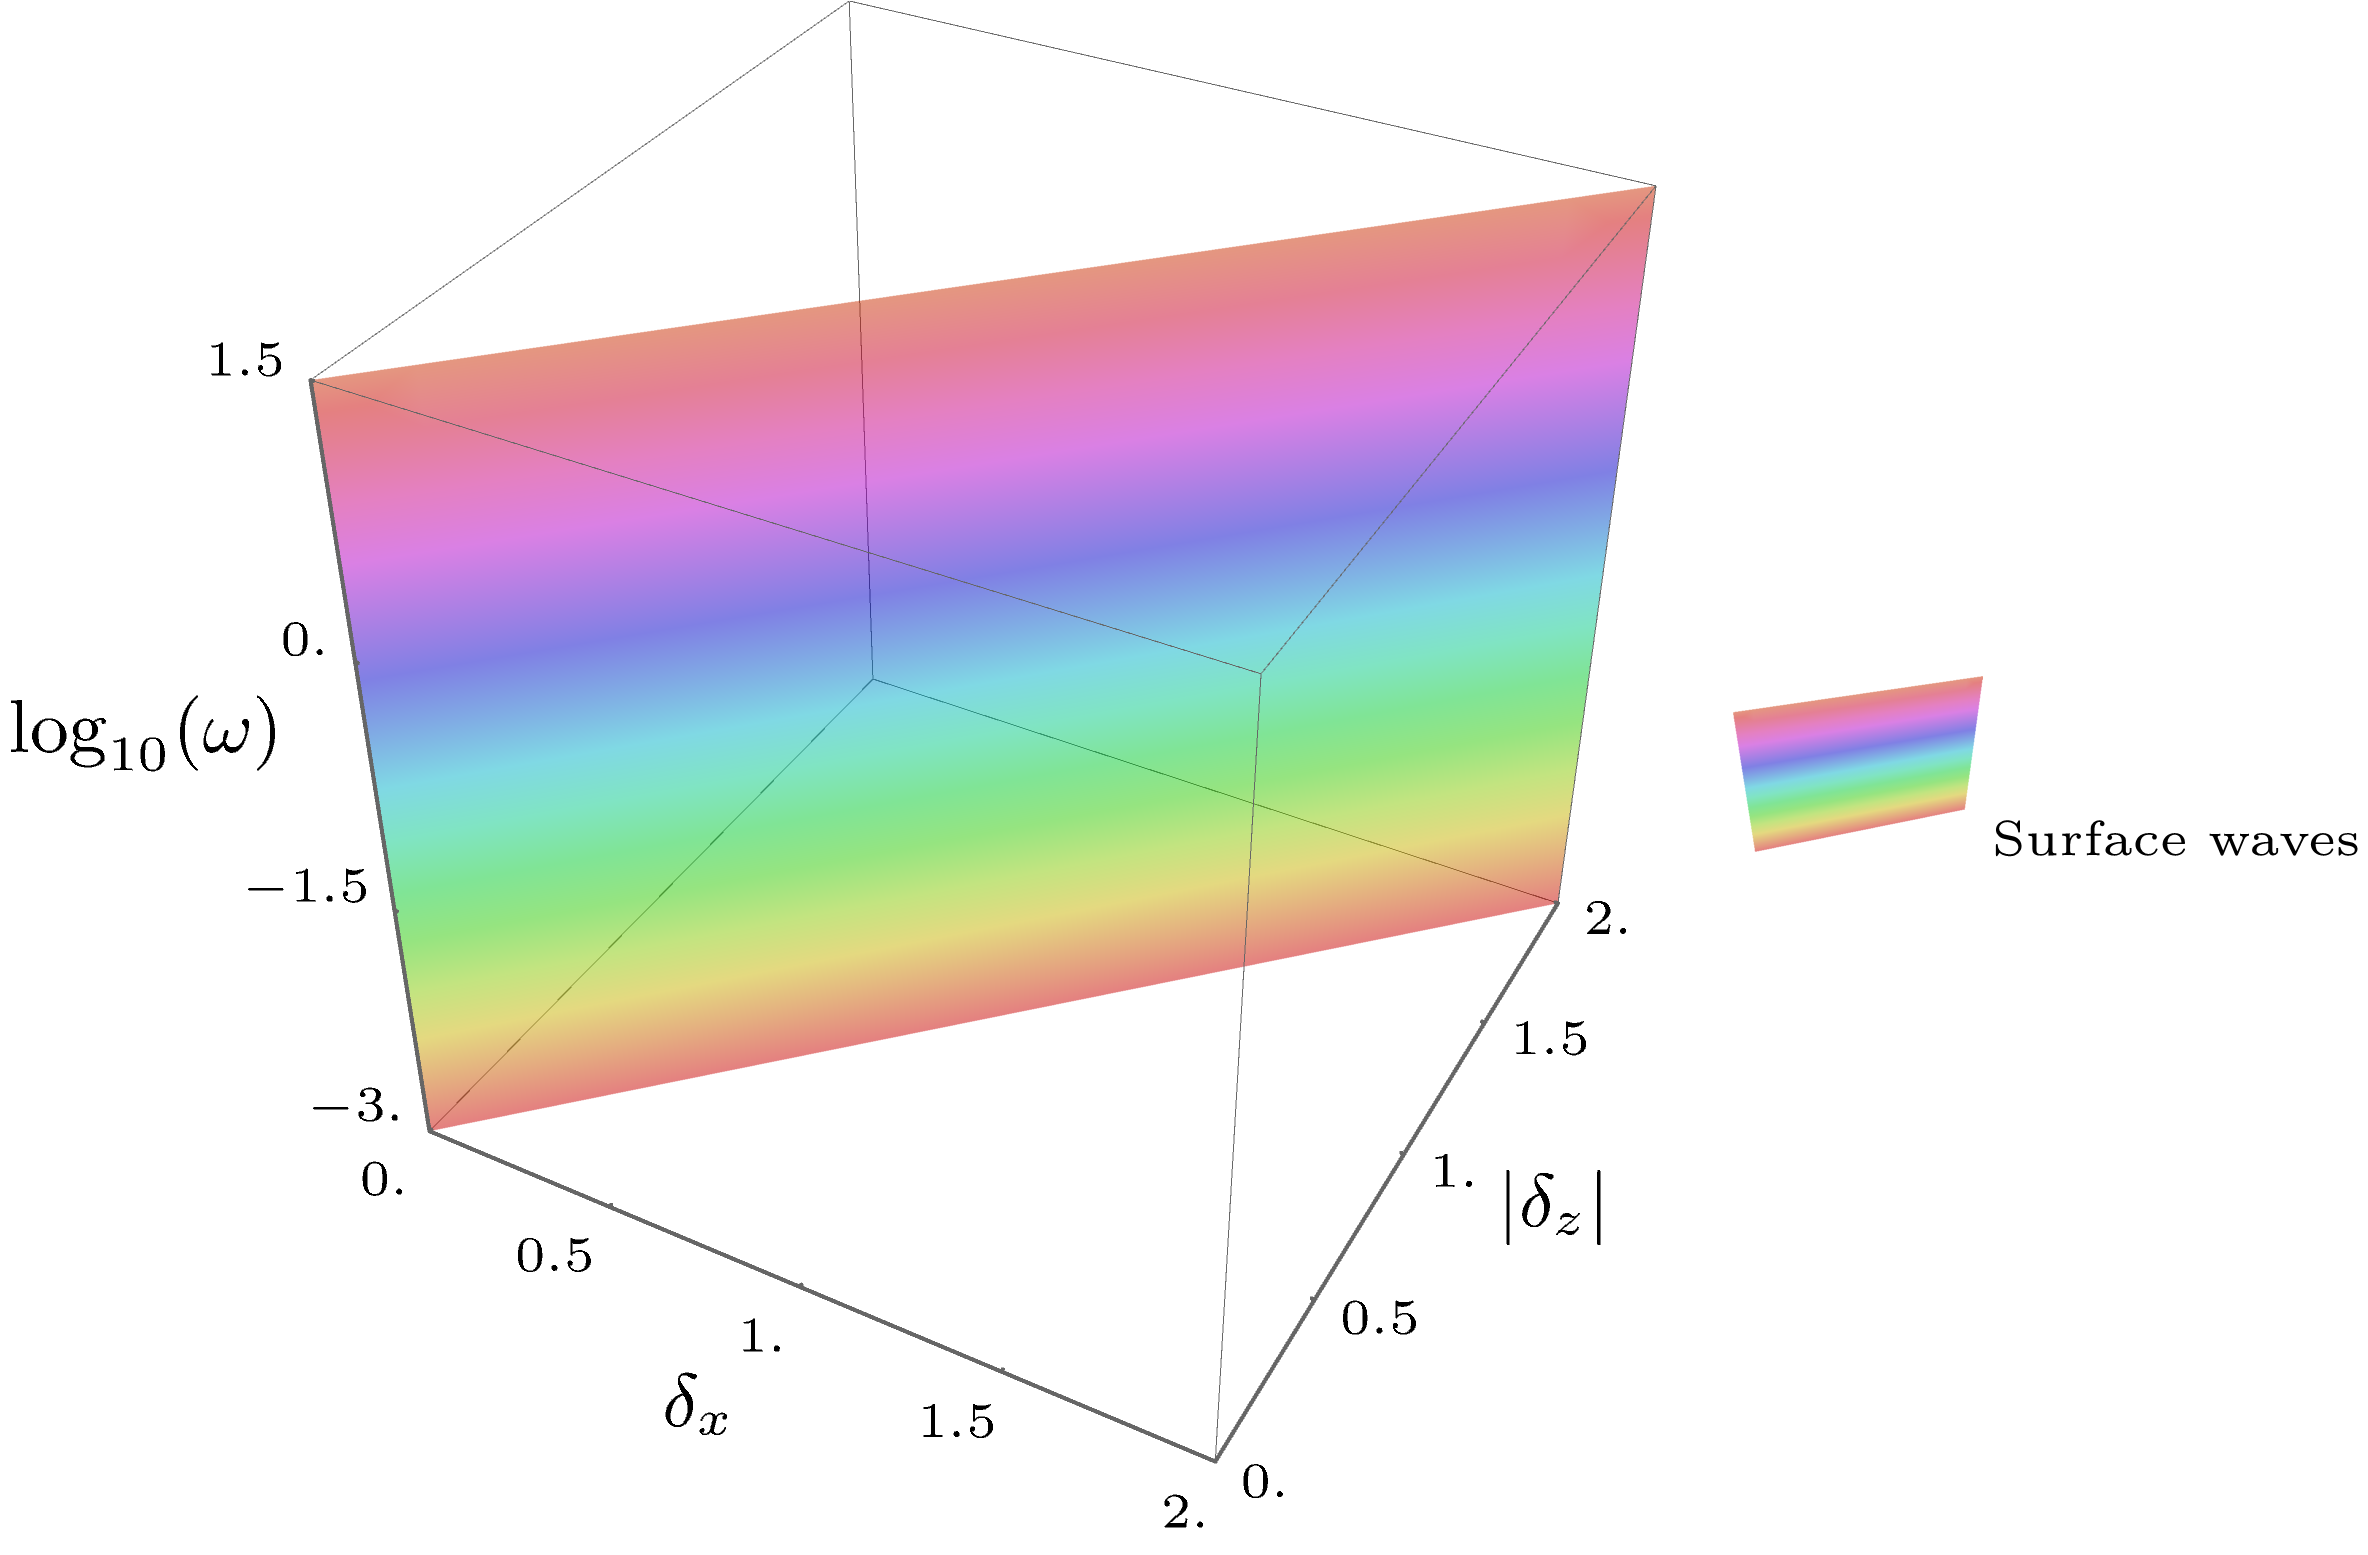
\includegraphics[width=0.35\linewidth]{FIGURES/unboundedwavesepsiepsa0.png}
	}
	\caption{Inner dispersion surfaces for the limit cases of (a) an incompressible ocean (b) an homogeneous ocean and (c) an incompressible and homogeneous ocean (in this case, the wave frequency is free, i.e., not constrained by the inner dispersion relation).}
	\label{FigFullsimplifiedcases}
\end{figure}
%
Approximate frequency values for modified internal and acoustic waves are summarized in Table \oldref{Summary_unbounded_IA} and Table \oldref{TableWavesolutions_modified} in dimensional form, for comparison with introductory Table \oldref{TableWave solutions}. Since the practical existence and characterization of modified surface waves is strongly dependent on boundary conditions, they are not summarized here but will be detailed in the next section.
%
\begin{table}[h]
\centerline{
\begin{tabular}{l|l|l}
	&Internal Waves&Acoustic Waves\\ \hline
a) ($\epsilon_i=\epsilon_a=0$)&X&X\\
b) ($\epsilon_i=0, \epsilon_a\ne 0$)&X&$\displaystyle \frac{\omega_+^2}{\omega_{aw}^2}\approx 1+\frac{\epsilon_a^4}{4(\delta_x^2+\delta_z^2)}$\\
c) ($\epsilon_i\ne 0, \epsilon_a = 0$)&$\displaystyle \frac{\omega_-^2}{\omega_{iwr}^2}\approx 1-\frac{\epsilon_i^4}{4(\delta_x^2+\delta_z^2)}$&X\\
d) ($\epsilon_i\ne 0, \epsilon_a \ne 0$)&$\displaystyle \frac{\omega_-^2}{\omega_{iwr}^2}\approx 1
-\frac{(\epsilon_i^2+\epsilon_a^2)^2\delta_z^2+(\epsilon_a^2-\epsilon_i^2)^2\delta_x^2}{4(\delta_x^2+\delta_z^2)^2}$&
$\displaystyle \frac{\omega_+^2}{\omega_{aw}^2} \approx 1+
\frac{(\epsilon_i^2+\epsilon_a^2)^2\delta_z^2+(\epsilon_a^2-\epsilon_i^2)^2\delta_x^2}{4(\delta_x^2+\delta_z^2)^2}
$
\\
\end{tabular}
}
\caption{Modified Internal and Acoustic waves in an unbounded ocean.}
\label{Summary_unbounded_IA}
\end{table}
\begin{table}[!h]
	\setlength{\extrarowheight}{15pt}
	\centerline{
		\begin{tabular} {p{5.3cm}|p{9cm}}
			Waves &  Frequency $(\Omega)$\\\hline
			Modified Acoustic Waves (MAW) &
$\displaystyle \Omega_{maw}^2=c_s^2(k_x^2+k_z^2)
\left[
1+\frac{1}{4(k_x^2+k_z^2)^2}\left(
\frac{k_z^2}{D_0^2}+\left(
\frac{g}{c_s^2}-\frac{N^2}{g}
\right)^2
k_x^2
\right)
\right]$\\[5mm]
Modified Internal Waves (MIW) & $\displaystyle \Omega_{miw}^2=\frac{N^2 k_x^2}{k_x^2+k_z^2}
\left[
1-\frac{1}{4(k_x^2+k_z^2)^2}\left(
\frac{k_z^2}{D_0^2}+\left(
\frac{g}{c_s^2}-\frac{N^2}{g}
\right)^2
k_x^2
\right)
\right]
$
	\end{tabular}}	
	\caption{Compressibility and stratification induced modifications to the usual dispersion relations given in Table \oldref{TableWave solutions}. $\Omega$ is wave angular frequency, $k_x$ and $k_z$ are the wavenumbers, $g$ is the acceleration of gravity, $N$ a reference Brunt-V\"ais\"al\"a frequency and $c_s$ the speed of sound. $D_0$ is the background density vertical scale, given by $1/D_0=N^2/g+g/c_s^2$}
	\label{TableWavesolutions_modified}
\end{table}
%\begin{table}[h]
%	\centerline{
%		\begin{tabular}{lll}
%			&Surface Waves\\
%			a) ($\epsilon_i=\epsilon_a=0$)&$\omega$ not specified and $\delta_{z,i}=\delta_x$\\
%			b) ($\epsilon_i=0, \epsilon_a\ne 0$)&$\displaystyle \frac{\omega_+^2}{\omega_{aw}^2}=1+\frac{\epsilon_a^4}{4(\delta_x^2+\delta_z^2)}$\\
%			c) ($\epsilon_i\ne 0, \epsilon_a = 0$)&$\displaystyle \frac{\omega_+^2}{\omega_{aw}^2}=1+\frac{\epsilon_a^4}{4(\delta_x^2+\delta_z^2)}$\\
%			d) ($\epsilon_i\ne 0, \epsilon_a \ne 0$)
%			&$\displaystyle \frac{\omega_+^2}{\omega_{aw}^2}=1+\frac{\epsilon_a^4}{4(\delta_x^2+\delta_z^2)}$\\
%		\end{tabular}
%	}
%	\caption{Modified Surface waves in an unbounded ocean. H: homogeneous, I: Incompressible, S: Stratified}
%\label{Summary_unbounded_S}
%\end{table}

In a more realistic bounded ocean, their existence is guaranteed only if their vertical scale is (much) smaller than the ocean depth $(|\delta_z| \gg 1)$ and if they do not interfere with the bottom or the surface of the ocean. The next section will investigate the impact of adding the boundary dispersion relation \ref{EqFullDisperb}.
%%%%%%%%%%%%%%%%%%%%%%%%%%%%%%%%%%%%%%%%%%%%%%%%%%%%%%%%%%%%%%%%%%%%%%%%%%%%%

%%%%%%%%%%%%%%%%%%%%%%%%%%%%%%%%%%%%%%%%%%%%%%%%%%%%%%%%%%%%%%%%%%%%%%%%%%%
\section{Waves in a bounded ocean}
\label{SectionGraphic}
%%%%%%%%%%%%%%%%%%%%%%%%%%%%%%%%%%%%%%%%%%%%%%%%%%%%%%%%%%%%%%%%%%%%%%%%%%%

\subsection{Graphical investigation of Modified Surface Waves (MSW), Modified Acoustic Modes (MAM) and Modified Internal Modes (MIM)}
\label{SubSectionPotBranches}
The compressible and stratified ocean is now supposed to be bounded. Wave solutions must consequently satisfy both the inner \ref{EqFullDispera} and boundary \ref{EqFullDisperb} dispersion relations. In phase space, they must lie at the intersections of the inner and boundary dispersion surfaces, which are plotted simultaneously on Figure \oldref{FigDispSolutions}.
%
\paragraph{Branches of the boundary dispersion surface}
%
\begin{figure}[h]
	\centering
	\subfloat[][]{
	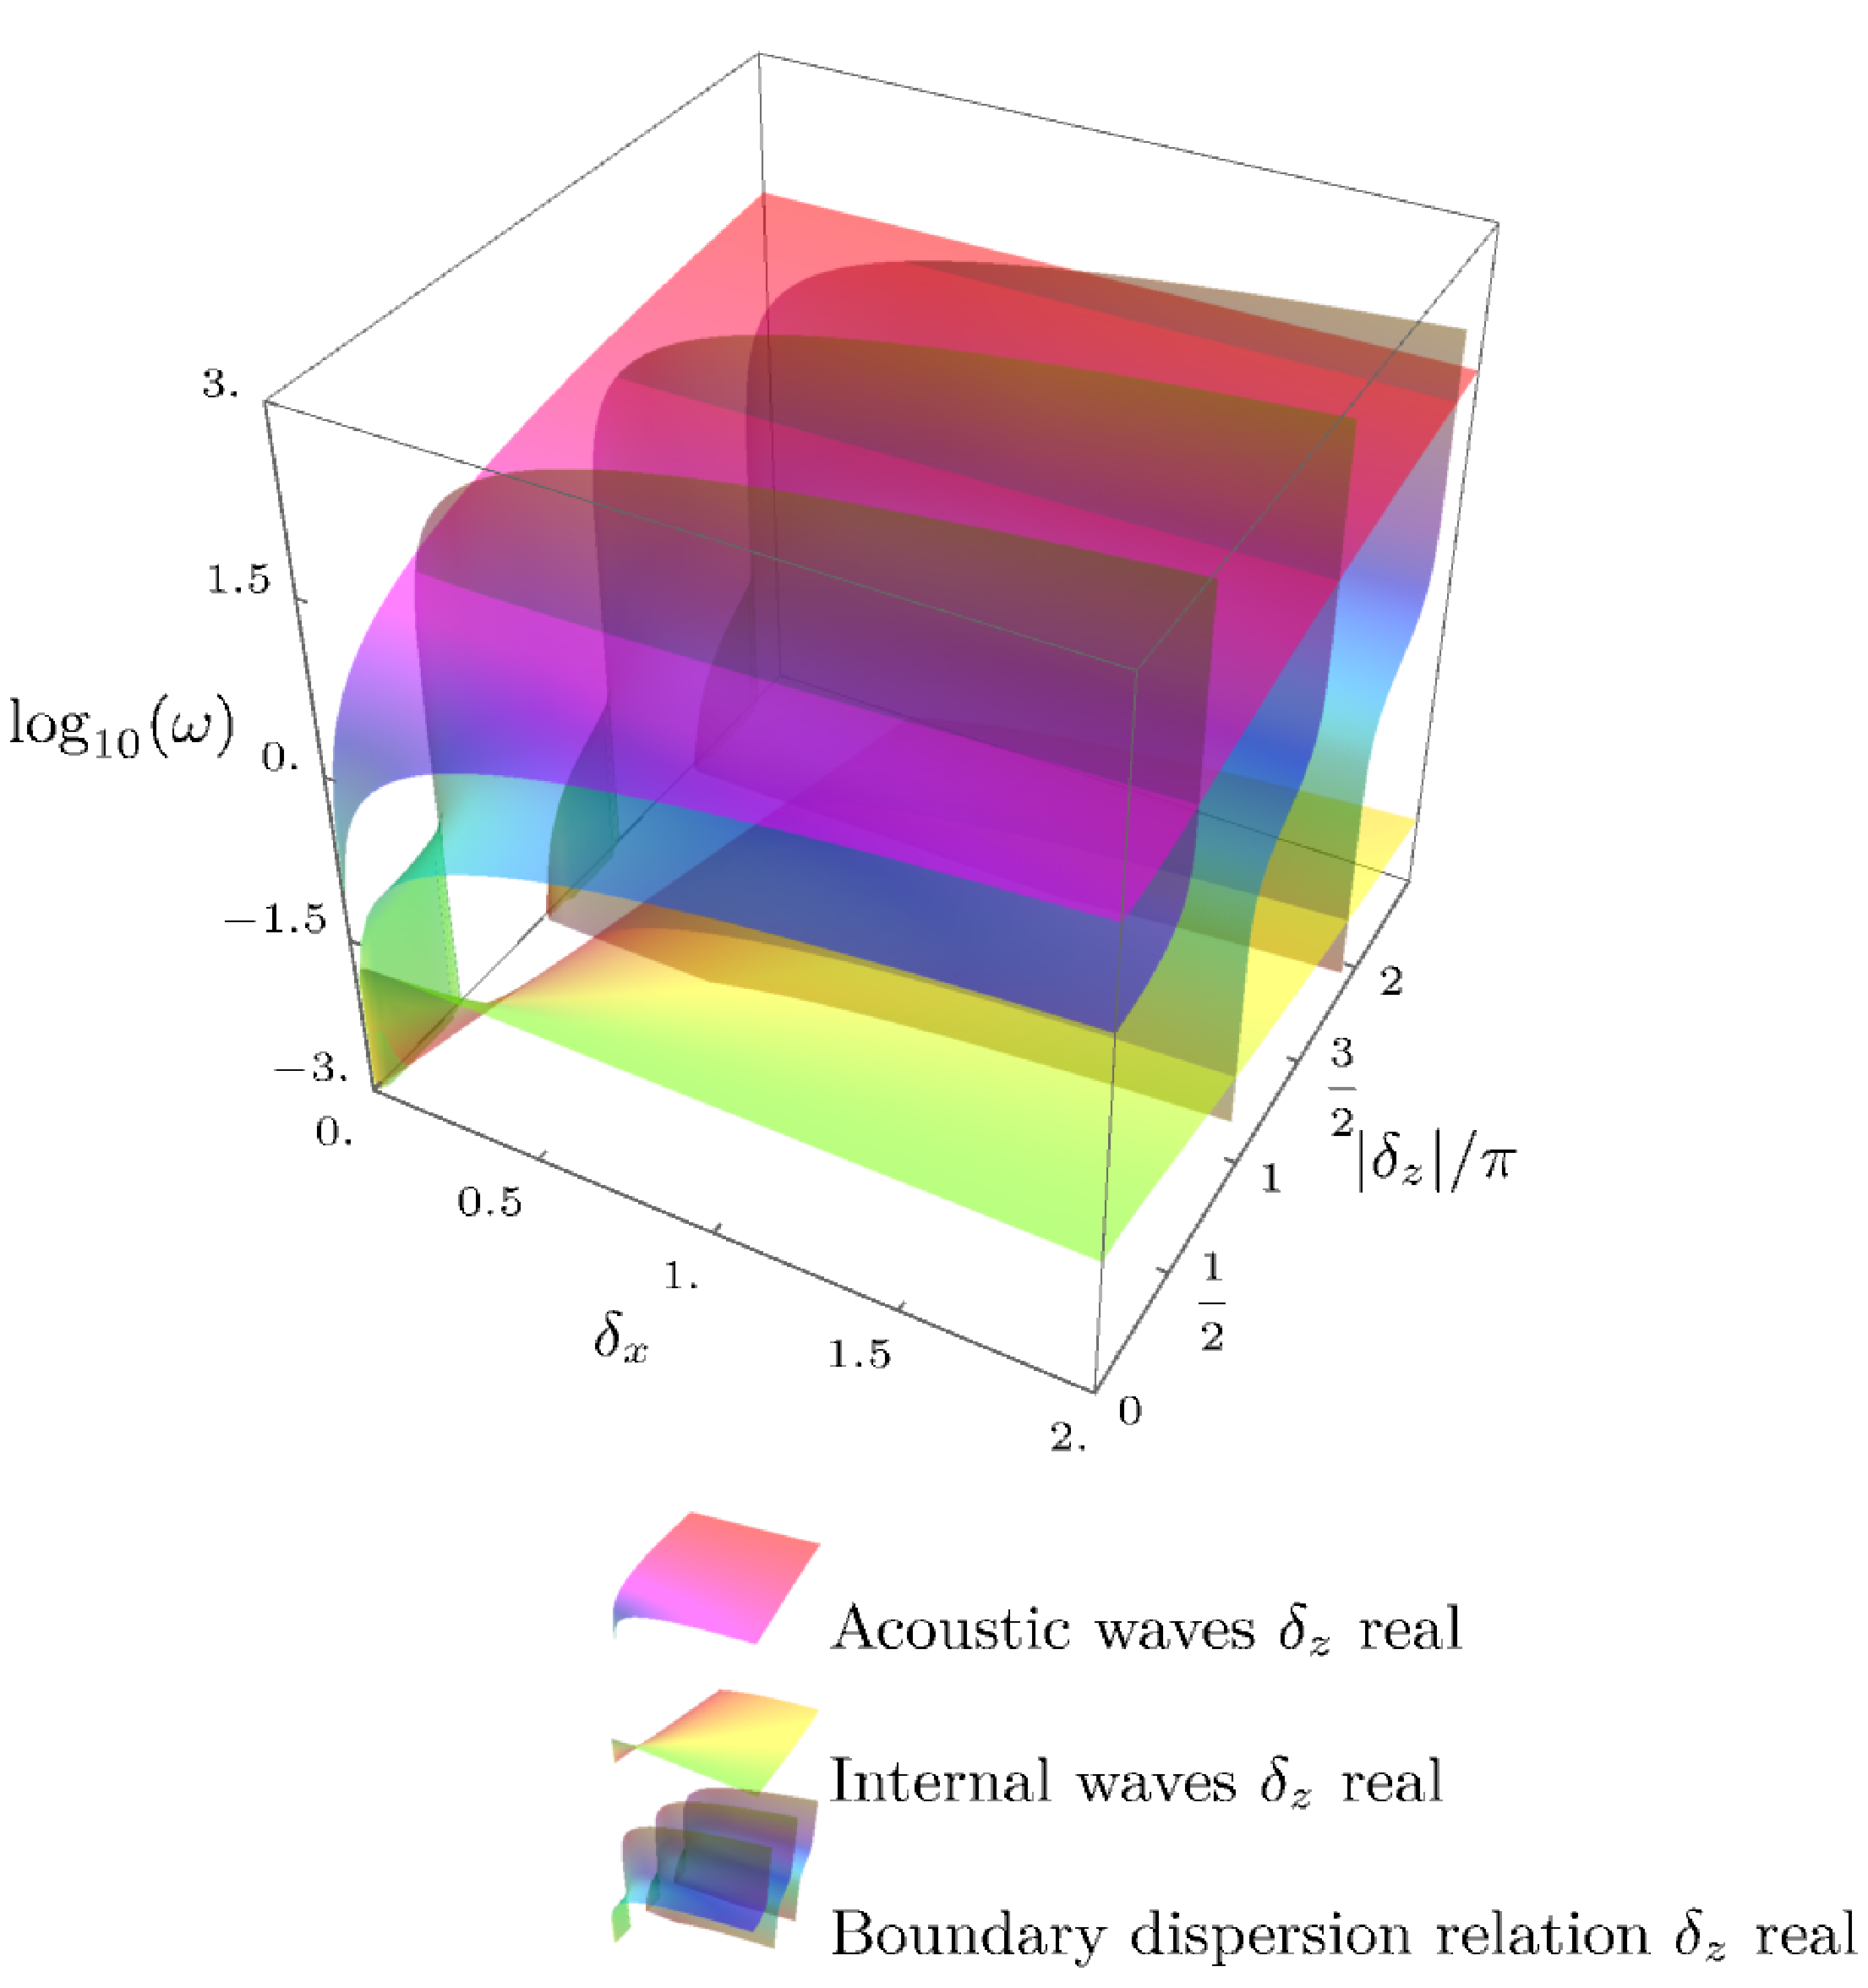
\includegraphics[width=0.45\linewidth]{FIGURES/boundedreal.png}
}
	\centering		
	\subfloat[][]{
		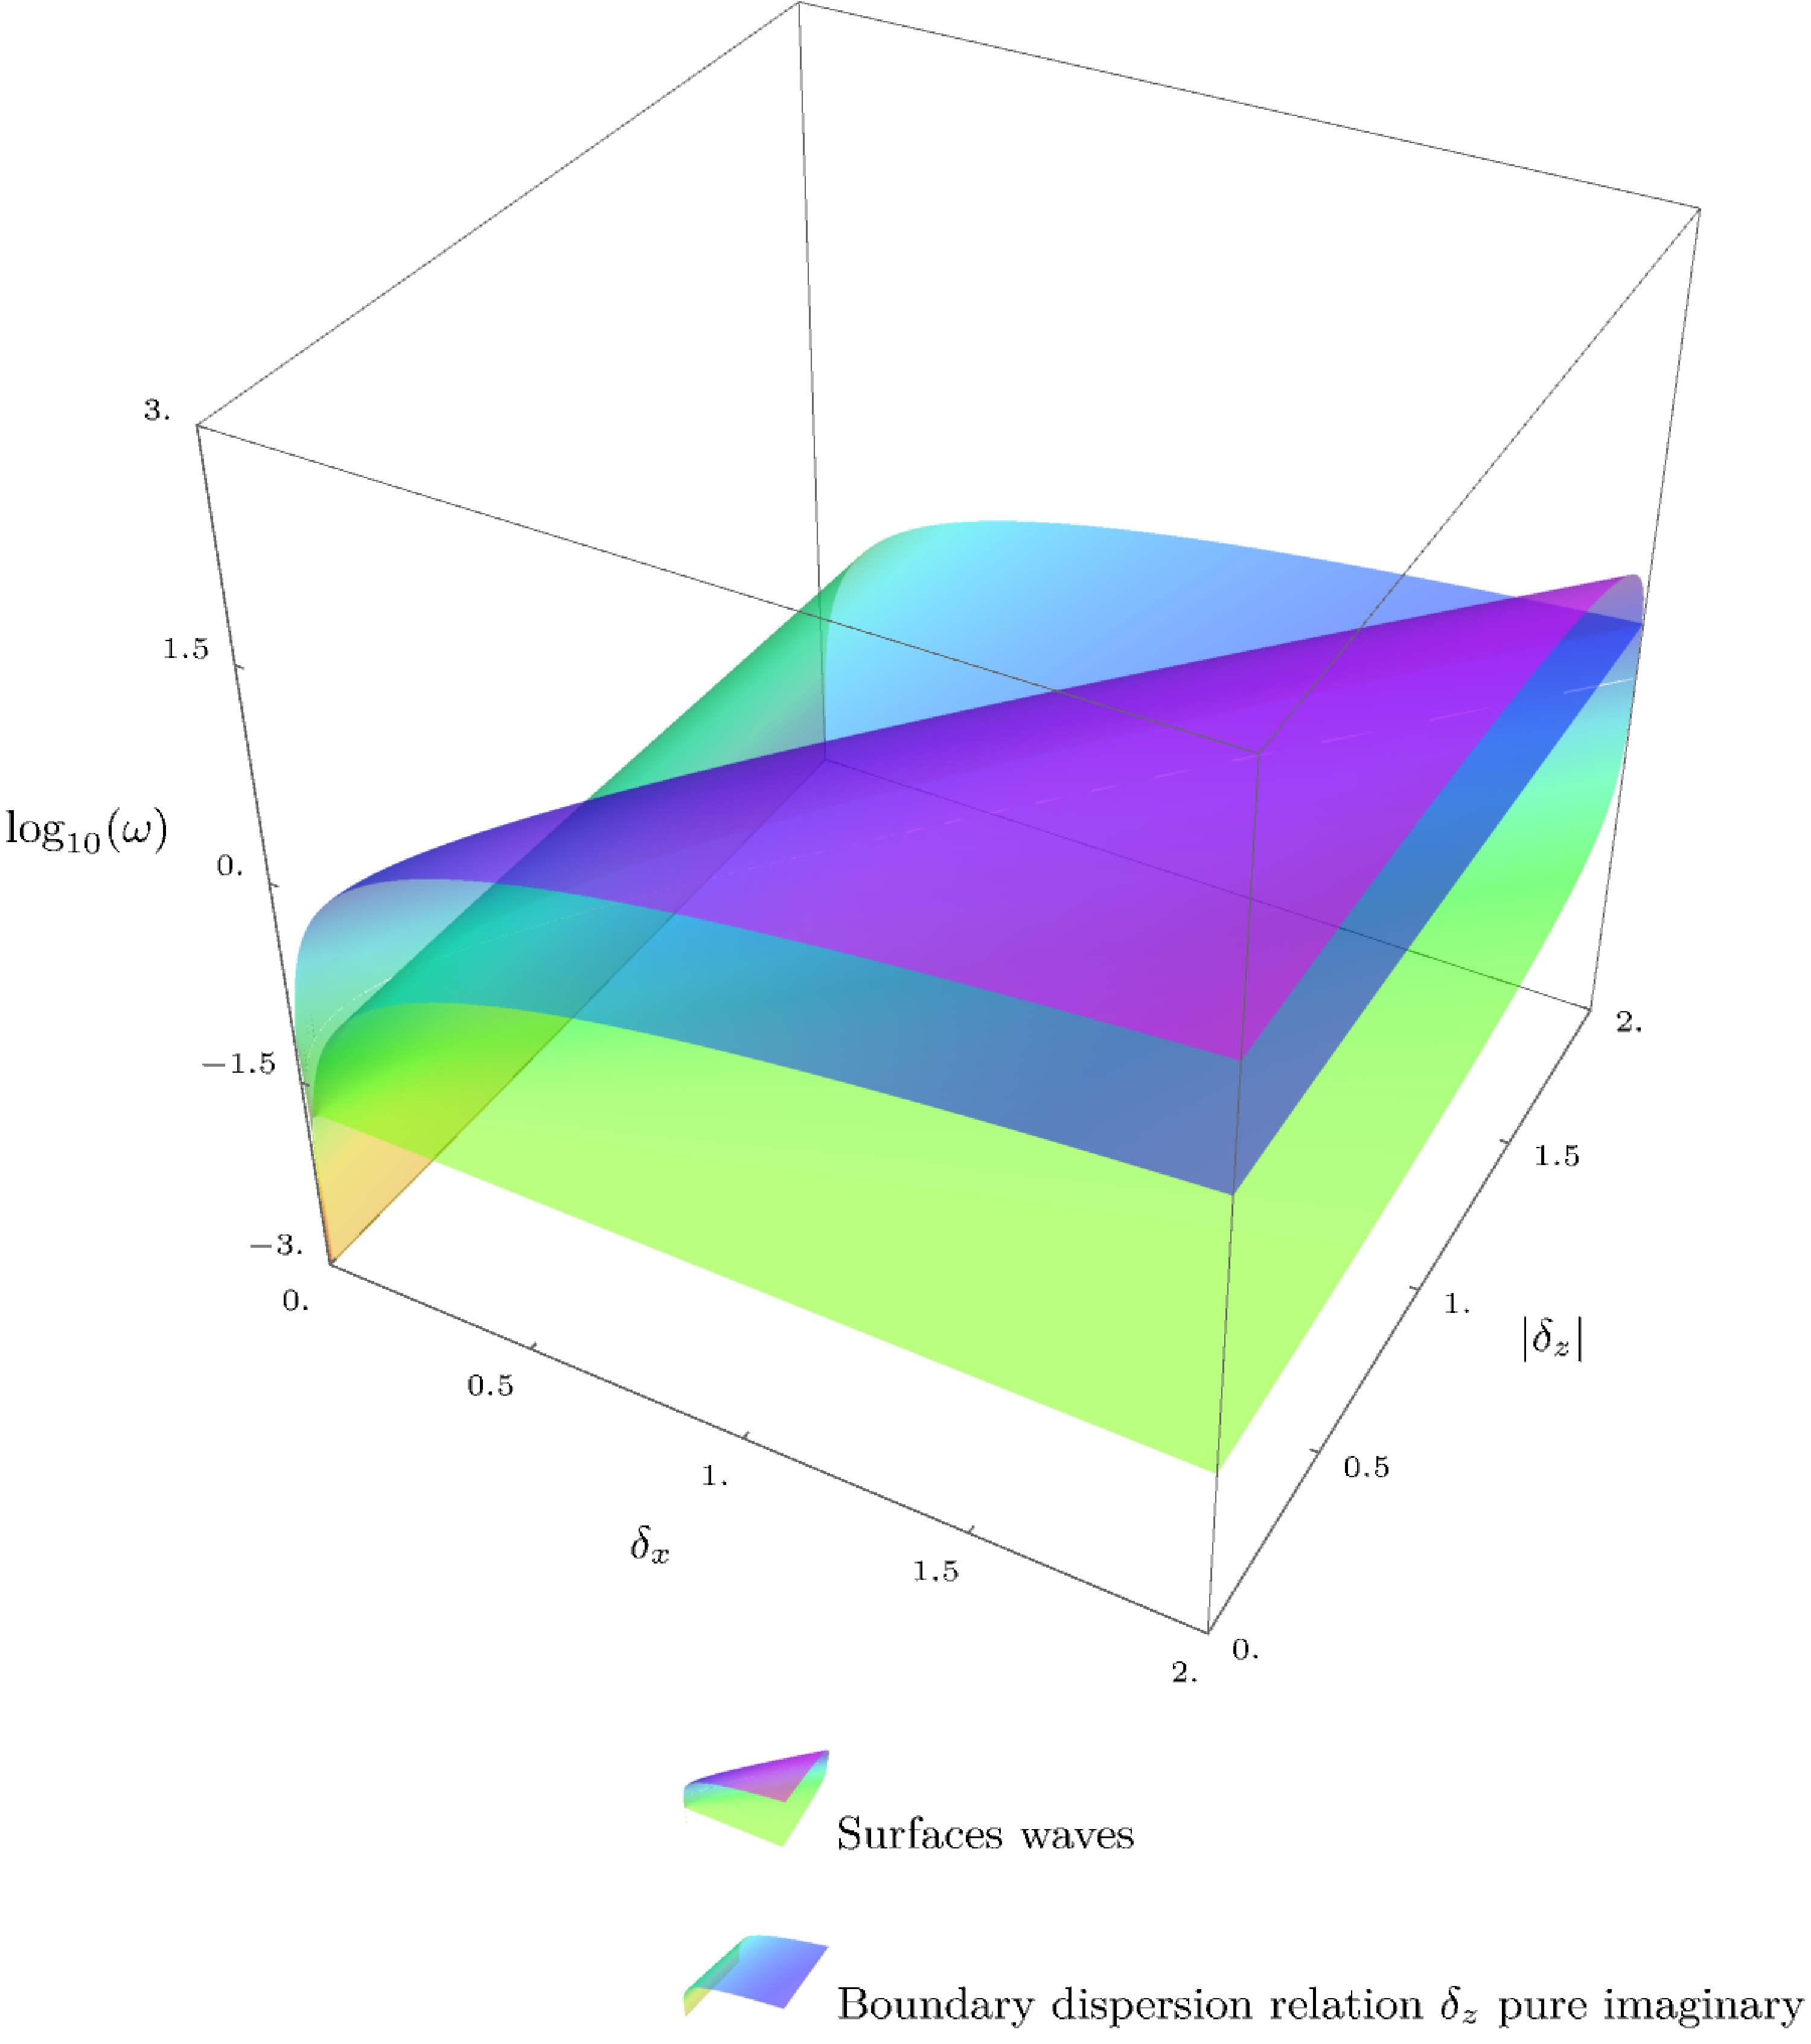
\includegraphics[width=0.45\linewidth]{FIGURES/boundedimaginary.png}
}
	\caption{\textit{Dispersion surfaces in $(\delta_x,\ \delta_z,\log_{10}(\omega))$  space and wave solutions.\\
	%	Wave solutions. Polychrome surfaces: Inner dispersion surface for real $\delta_z$ (acoustic and gravity branches). Blue: Boundary dispersion surface. Black points: acoustic wave (upper branch) and internal wave solutions (lower branch).
		%
			 (a) Wave solutions with real $\delta_z$. Polychrome surfaces: inner dispersion surfaces (acoustic and internal branches) and Boundary dispersion surface.\\
			 (b) Wave solutions with purely imaginary $\delta_z$. Polychrome surfaces: inner dispersion surface (surface gravity-wave branch) and Boundary dispersion surface.
		%	 (c) Wave solutions in the vicinity of the origin. Polychrome surface: Lower (respectively upper) $\delta_x$: inner dispersion surface for real $\delta_z$ (pure imaginary $\delta_z$). Blue: Boundary dispersion surface. Black (red) points: surface wave solutions.\\
		%	 (d) Wave solutions with both real and pure-imaginary wave-numbers as given in (a) and (b).
	}
}
\label{FigDispSolutions}
\end{figure}
%\begin{figure}[!h]
%	\centering		
%	\begin{subfigure}{0.45\linewidth}
%		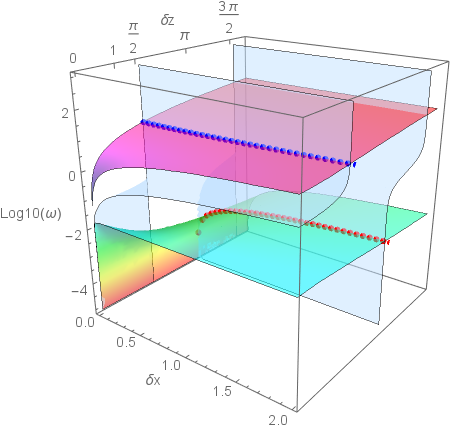
\includegraphics[width=1\linewidth]{FIGURES/Fig_Inter_Real.png}
%		\caption{}
%	\end{subfigure}
%	~
%	\centering
%	\begin{subfigure}{0.45\linewidth}
%		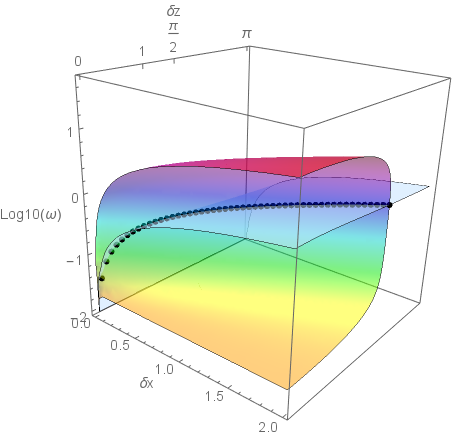
\includegraphics[width=1\linewidth]{FIGURES/Fig_Inter_Imag.png}
%		\caption{}
%	\end{subfigure}
%	
%	\begin{subfigure}{0.45\linewidth}
%		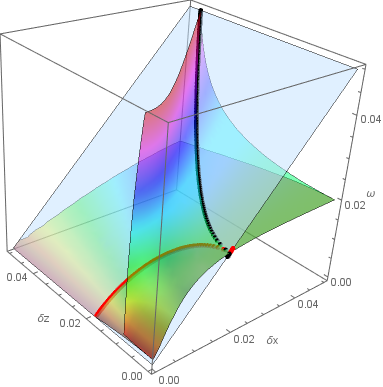
\includegraphics[width=1\linewidth]{FIGURES/Fig_Inter_All_zoom5.png}
%		\caption{}
%	\end{subfigure}
%	~
%	\begin{subfigure}{0.45\linewidth}
%		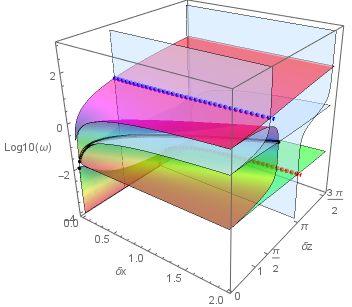
\includegraphics[width=1\linewidth]{FIGURES/Disp_Full_all.png}
%		\caption{}
%	\end{subfigure}
%
%	\caption{\textit{Dispersion surfaces in $(\delta_x,\ \delta_z,\ Log_{10}(\omega)$ or $\omega)$  space and wave solutions.\\
%Wave solutions. Polychrome surfaces: Inner dispersion surface for real $\delta_z$ (acoustic and gravity branches). Blue: Boundary dispersion surface. Black points: acoustic wave (upper branch) and internal wave solutions (lower branch).
%%
%%	 (a) Wave solutions with real $\delta_x$. Polychrome surfaces: Inner dispersion surface for real $\delta_z$ (acoustic and gravity branches). Blue: Boundary dispersion surface. Black points: acoustic wave (upper branch) and internal wave solutions (lower branch).\\
%%	 (b) Wave solutions with pure imaginary $\delta_x$. Polychrome surface: Inner dispersion surface for pure imaginary $\delta_z$ (surface gravity-wave branch). Blue: Boundary dispersion surface. Red points: surface wave solutions.\\ 
%%	 (c) Wave solutions in the vicinity of the origin. Polychrome surface: Lower (respectively upper) $\delta_x$: inner dispersion surface for real $\delta_z$ (pure imaginary $\delta_z$). Blue: Boundary dispersion surface. Black (red) points: surface wave solutions.\\
%%	 (d) Wave solutions with both real and pure-imaginary wave-numbers as given in (a) and (b).
% }
% }
%	\label{FigDispSolutionsold}
%\end{figure}
%For pure-imaginary vertical wave numbers, the inner dispersion surface is folded both for large and small pulsations. For real vertical wave-numbers branches are present in the upper and lower regions as could be expected by adding the transformations already observed in figure \ref{FigFullHomogeneous} when $\epsilon_i$ and $\epsilon_a$ were separately non zero. In the large-pulsation region, the upper branch of the inner dispersion surface is similar to figure (\oldref{FigFullHomogeneous}.c) and, once again, could not be distinguished from the $\omega^2=\omega_a^2$ surface. The same is true in the small-pulsation region where the lower branch of the inner dispersion surface could this time not be distinguished from the $\omega^2=\omega_i^2$ surface. This is a consequence of the separation of the roots of the inner dispersion relation \ref{solseq} or equivalently of the separation of the upper, acoustic and lower, acoustic branches already observed in figure \ref{FigFullHomogeneous}: when $\epsilon_i$ and $\epsilon_a$ are simultaneously non zero, MAW and MIW can simultaneously propagate. Nevertheless, relations \ref{DispAcousDT} and \ref{DispRaysDT} show that at higher order in this small parameters, their dispersion relations are modified by the stratification and/or the compressibility of the ocean. Figure \oldref{FigDispSolutions}.d additionally provides all dispersion surface branches on the same plot. It confirms inequality \ref{RelInequal}. The inner-dispersion surface for pure-imaginary wave-numbers is bounded by the same surfaces for real wave-numbers.\\
For real vertical wavenumbers ($k_z\in\mathbb{R}$, Figure \oldref{FigDispSolutions}a), the boundary dispersion surface is a piecewise surface. It includes several branches that are vertical (in the $(\delta_x, \delta_z, \log_{10}(\omega)$) space) at $\delta_z \approx n\pi$ (small values of $\omega$) and at $\delta_z \approx \pi/2+m\pi$ (large values of $\omega$), with $n\in\mathbb{N}^\ast$ and $m\in\mathbb{N}$. The intersection of these branches with the inner dispersion relation surfaces result in a number of constrained vertical wavenumbers (according to the values of $n$ and $m$), the resulting wave solutions will thus be called {\it modes}. The two intersections correspond to {\it Modified Internal Modes (MIM),  $n\in\mathbb{N}^\ast$} and to {\it Modified Acoustic Modes (MAM), $m\in\mathbb{N}$}.\\
For purely imaginary wavenumbers (Eq. \ref{EqFullDisperbi}), the boundary surface (Figure \oldref{FigDispSolutions}b) looks like an horizontal hyperbolic surface which intersects the surface waves surface. Far from the origin $(\delta_x,\delta_z)=(0,0)$, at the intersection points, $|\delta_z|$ is close to $\delta_x$.
%\textit{Numerical approximations of wave solutions in a bounded ocean:}\\
%Figure \ref{FigDispSolutions} confirms for this model of compressible, stratified, free-surface ocean, the existing of three types of intersections between the inner and boundary dispersion surfaces and, as a consequence, three regions of phase-space where waves can propagate in a bounded ocean. These intersections are shown by three lines of color points. The black-point intersection corresponds to wave-solutions propagating with a pure imaginary vertical wave-number in the middle-range pulsation region (figures \oldref{FigDispSolutions}.b, c and d). These are surface (edge) vertically-vanishing waves propagating in a compressible, stratified ocean, hereafter named Modified Surface Waves (MSW). Figure \oldref{FigDispSolutions}.d shows that they occupy a region of phase-space where the inner dispersion surface is approximately vertical and tangent to the $\delta_x\approx\delta_{z,i}$ plane meaning that the influence of compressibility and stratification (gravity) are both small. 
%
%The red and blue lines of points indicate that two remaining wave-solutions are possible, this time with real vertical wave-numbers. One (blue points) is an intersection of the boundary dispersion surface with the upper acoustic branch of the inner dispersion surface (figures \oldref{FigDispSolutions}.a, c and d), the other (red points) is an intersection of the same boundary dispersion surface with the lower stratification branch of the inner dispersion surface (figures \oldref{FigDispSolutions}.a and d). Since in both cases, vertical wave-numbers are quantified ($\delta_z = \pi/2+m\pi$ and $\delta_z \approx n\pi$), the resulting wave solutions can be associated to respectively Modified Acoustic Modes (MAM) and Modified Internal Modes (MIM), these modes being modified by both compressibility and stratification (gravity).\\
\paragraph{Long-wave solutions}
For long waves ($|\delta_z| \ll 1$), the boundary dispersion surfaces for real and purely imaginary $\delta_z$ coincide. Indeed the development of the boundary relation is well approximated by $\omega^2\approx \delta_x^2$ in both cases (a better approximation is given in Eq. \ref{eqomegalongwavereal}).
Figure \oldref{FigDisLongpSolutions} shows the different branches close to the origin $(\delta_x, \delta_z)=(0,0)$. The acoustic waves surface is not shown since it does not intersect the boundary dispersion surface near the origin (as proved in \S\oldref{SubSectionLongWavesrealdz}).
\begin{figure}[!h]
	\centering		
	%	\begin{subfigure}{0.45\linewidth}
	%		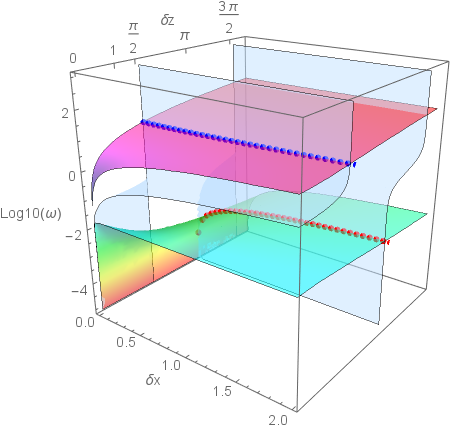
\includegraphics[width=1\linewidth]{FIGURES/Fig_Inter_Real.png}
	%		\caption{}
	%	\end{subfigure}
	%	~
	%	\centering
	%	\begin{subfigure}{0.45\linewidth}
	%		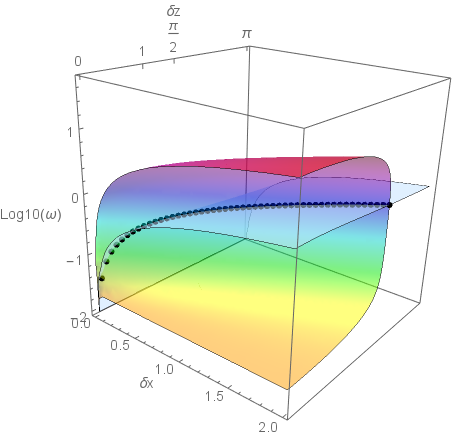
\includegraphics[width=1\linewidth]{FIGURES/Fig_Inter_Imag.png}
	%		\caption{}
	%	\end{subfigure}
	%	
	%	\begin{subfigure}{0.45\linewidth}
		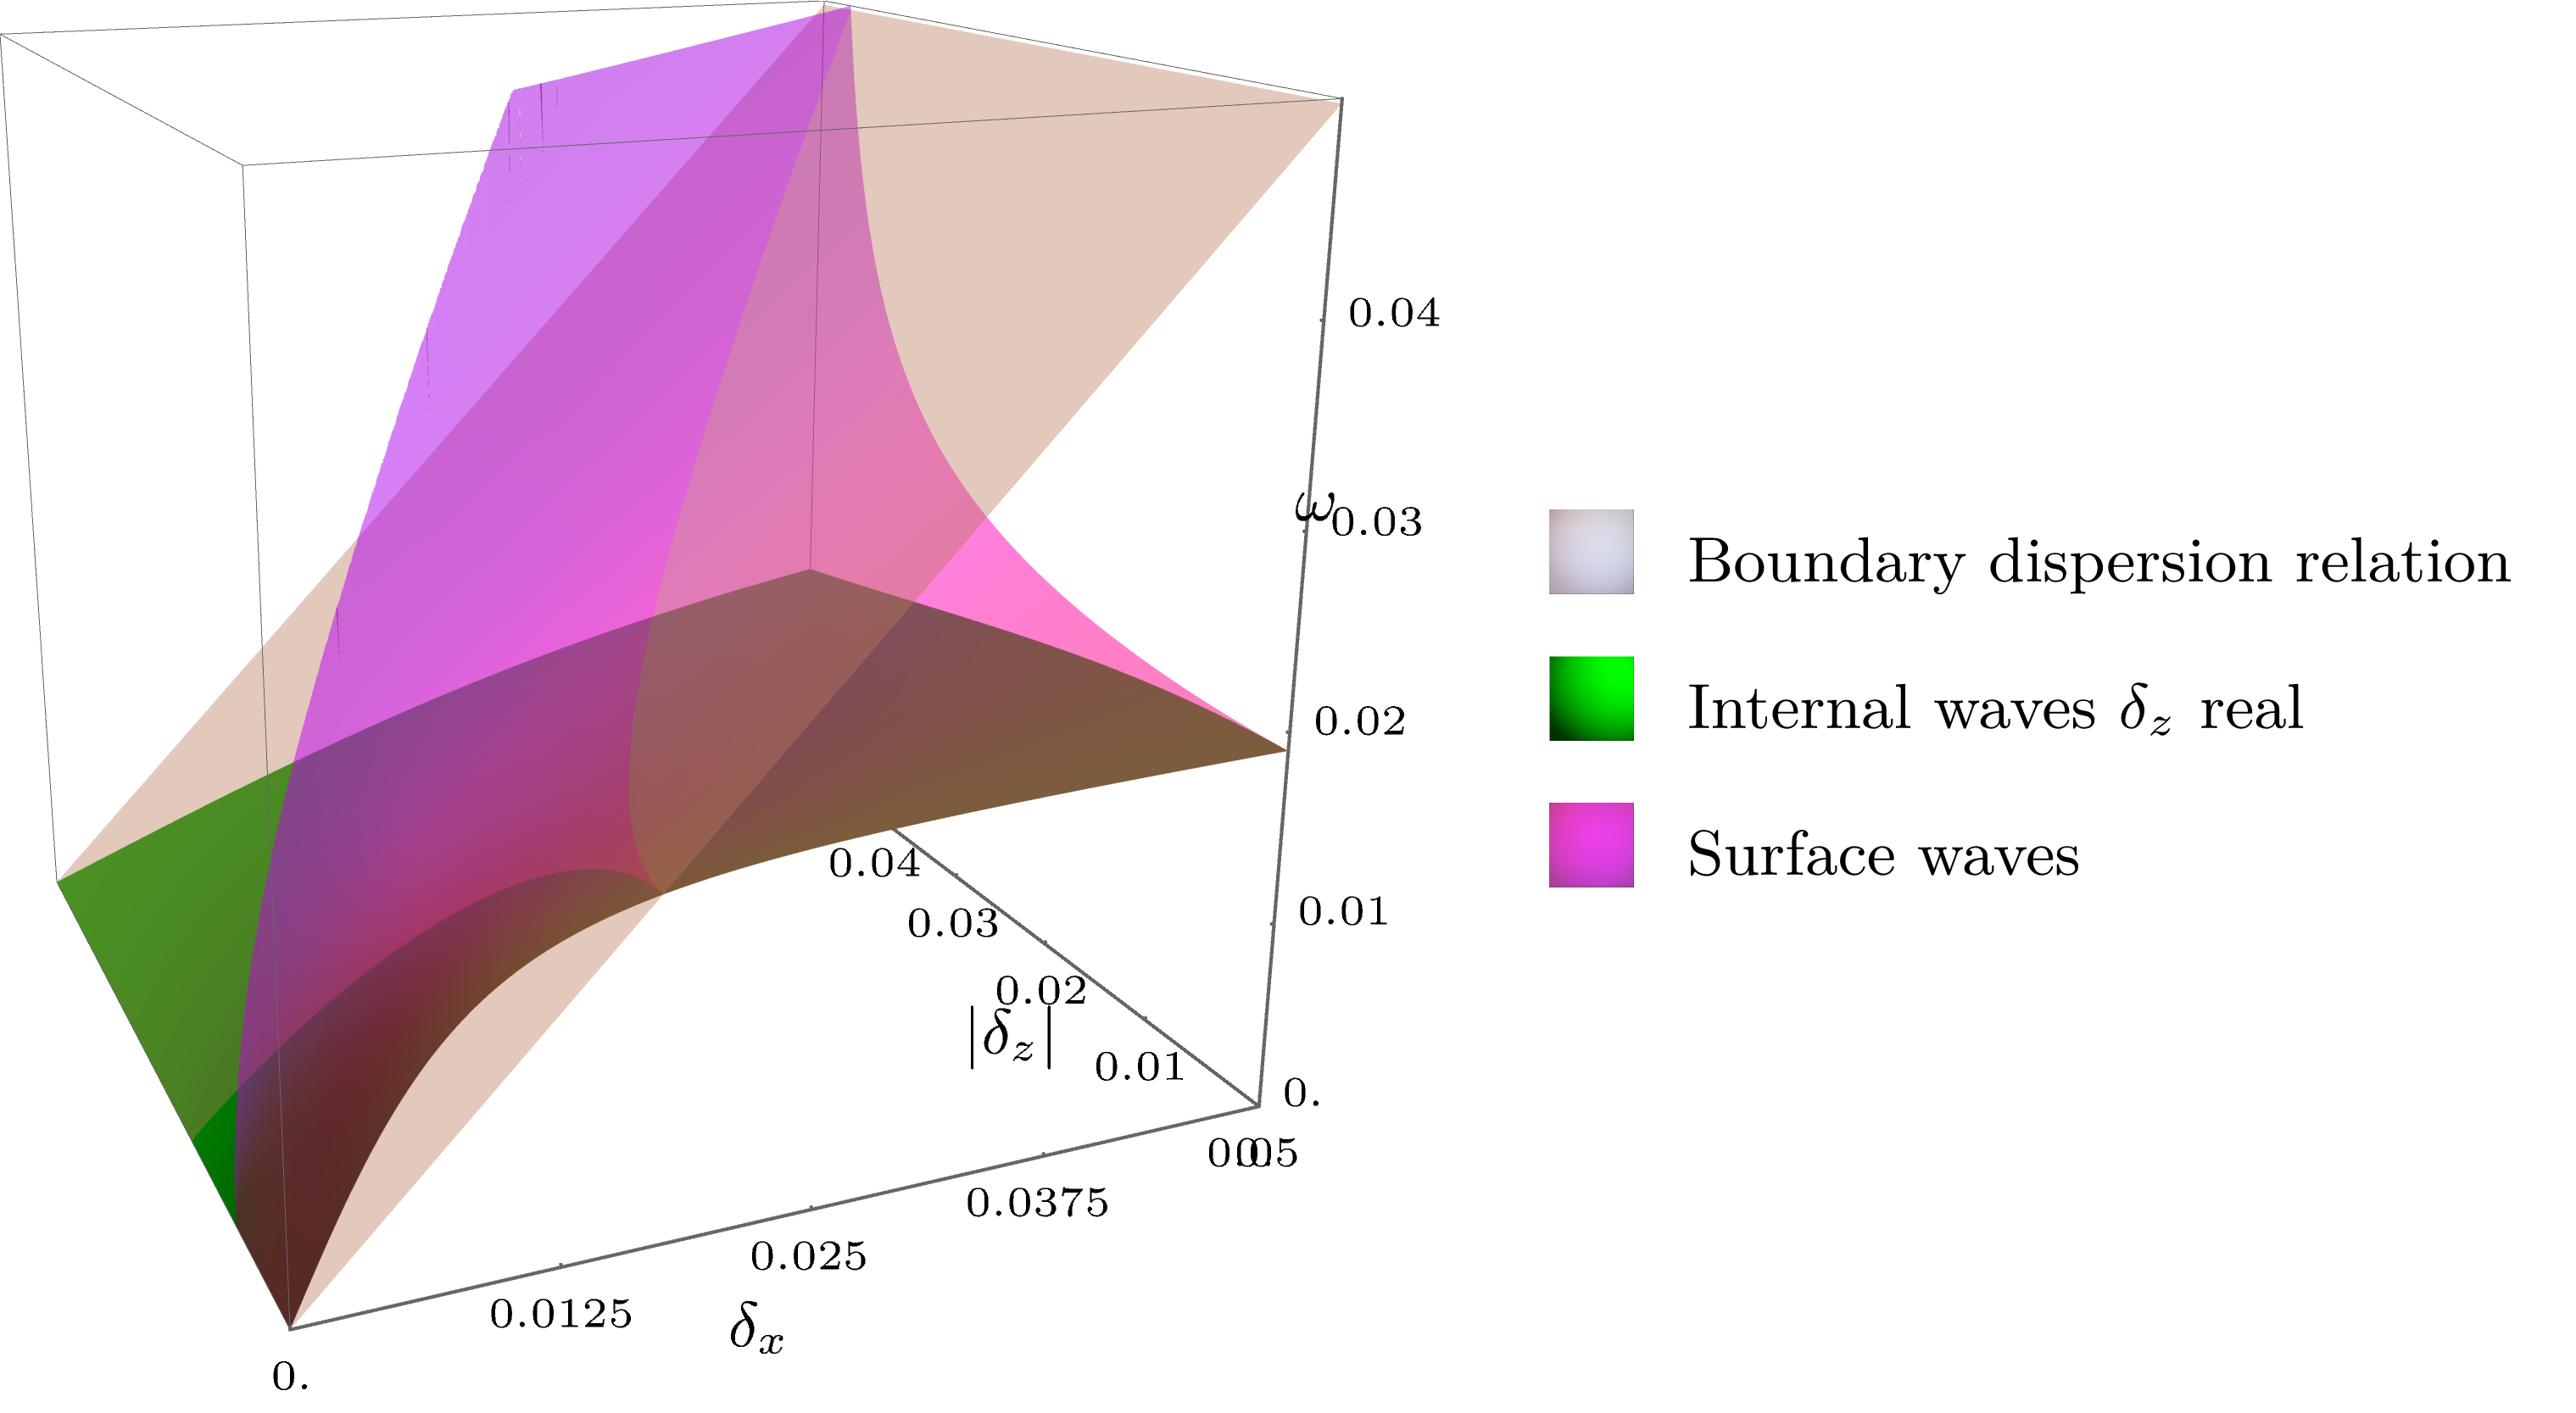
\includegraphics[width=0.6\linewidth]{FIGURES/boundedorigin.png}
	%		\caption{}
	%	\end{subfigure}
	~
	%	\begin{subfigure}{1.\linewidth}
	%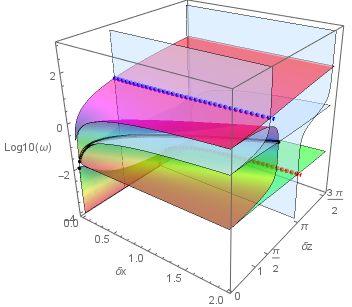
\includegraphics[width=1\linewidth]{FIGURES/Disp_Full_all.png}
	%		\caption{}
	%	\end{subfigure}
	
	\caption{\textit{Dispersion surfaces in $(\delta_x, \delta_z, \omega$) space and wave solutions in the vicinity of the origin. Polychrome surfaces: inner dispersion surfaces (internal and surface branches) and Boundary dispersion surface.
		}
	}
	\label{FigDisLongpSolutions}
\end{figure}
While for very small values of $\delta_x$, the boundary dispersion surface intersects the internal waves branch (with $\delta_z$ real), for larger values, it intersects the surface waves branch (with $\delta_z$ pure imaginary). As will be shown in section \oldref{SubSectionLongWavesrealdz}, the switch between the two intersections is at a value of $\delta_x=\delta_{x,0}\approx \epsilon_i$ (and for a vanishing vertical wavenumber $\delta_z=0$).
%In this figure \oldref{FigDisLongpSolutions}, the black-point intersection is the continuation for small wave-numbers of the MSW intersection in Figure \oldref{FigDispSolutions}b whereas the red-point intersection is not connected to the MIM intersection shown in Figure \oldref{FigDispSolutions}a. This continuous-by-part intersection leads to wave-solutions whatever $\delta_x$ in this region. For small values of $\delta_x$ the solution is given by the MIM branch (red points) whereas for larger values of $\delta_x$ it is given by the MSW branch (black points) and the vertical wavenumber vanishes in between these solutions.
\\
{\color{red}remarque ci-dessous: je vous laisse rephraser ... Duko dit (comme nous en fait) que la frequence du mode barotrope sature à $\epsilon_i$. (la phrase ci-dessous laisse penser qu'on est pas d'accord avec ca). Par contre, l'ami Duko a l'air de dire (cf Fig9.) que ce mode barotrope existe même pour des valeurs "grandes" de $\delta_x$ (ce qui parait complètement débile, puisque dans ce cas, elles sont où les ondes de surface non hydro classiques ?, quel gros naze ce Duko), alors que nous on montre que c'est seulement pour $\delta_x\le \epsilon_i$ et qu'ensuite ça passe dans la branche ondes de surface (et bien sûr on n'aurait eu que cette branche si on était partis des eqns.  Boussinesq, incompressible, comme dans les "Textbooks") cites par Dukowicz.}
Interestingly,  and contrary to conclusions in \cite{dukowicz_2013}, the barotropic mode pulsation cannot saturate at the buoyancy pulsation for increasing horizontal wavenumber $\delta_x$ but transforms into a vertically evanescent surface wave, while its vertical number switches from real to purely imaginary.
\paragraph{Summary}
In the context of a bounded ocean, three types of wave solutions spreading on the three branches of the inner dispersion surface have thus been identified graphically: internal gravity (in a stratified ocean), acoustic (in a compressible ocean) and surface waves (in a free-surface ocean) and satisfying at the same time the boundary dispersion relation. They will be investigated in the next subsections, where analytical expressions are systematically derived using Taylor expansions of the general roots $\omega_{\pm}$ with respect to small parameters $(\epsilon_i,\ \epsilon_a)$, leading to simple approximations of wave dispersion relations. When necessary, asymptotic relations are derived with respect to $\delta_x$, $\delta_z$ or $\omega$. The Taylor expansions additionally give indications on how usual wave solutions can be modified by gravity and stratification $(\epsilon_i)$, and/or by compressibility $(\epsilon_a)$.
%%%%%%%%%%%%%%%%%%%%%%%%%%%%%%%%%%%%%%%%%%%%%%%%%%%%%%%%%%%%%%%%%%%%%%%%%%%%%
\subsection{Real $\delta_z$: modified internal and acoustic waves}
As shown in \S\oldref{realwavenumber}, as long as $\delta_z$ is not close to zero, the upper (acoustic) and lower (gravity) branches of the inner dispersion surface for real $\delta_z$ are well-separated and the MAM and MIM solutions can thus be studied independently for real vertical wavenumbers. The case of long waves with $\delta_z \approx 0$ is discussed in subsection \oldref{SubSectionLongWavesrealdz}.
%
\subsubsection{Development of internal-gravity modes modified by compressibility (MIM)}
\label{SubSectionGraphicMIW}
%%%%%%%%%%%%%%%%%%%%%%%%%%%%%%%%%%%%%%%%%%%%%%%%%%%%%%%%%%%%%%%%%%%%%%%%%%%%%
%The mode-0 (barotropic) MIM solution will be investigated in section \ref{SubSectionGraphicMSW} and, as a consequence, only solutions for not small vertical wave-numbers needs to be explored here.
Waves can propagate horizontally between the bottom and surface of the ocean as in a wave guide. Internal gravity modes are  well-known such examples \citep{gill_1982}. In the previous section, graphical inspections of wave solutions confirmed that gravity waves with constrained vertical wavenumbers could be found at the intersection of the inner and boundary dispersion surfaces.
We have also shown in \S\oldref{realwavenumber} that the root of the inner dispersion relation corresponding to internal gravity waves is well-approximated by $\omega_i^2$. Making $\omega^2(\delta_x) \approx\omega_i^2$ in the boundary dispersion relation \ref{EqFullDisperb} leads to 
%\[
%	   \label{DispSysIntModesab}
%	\omega^2(\delta_x) \approx\omega_i^2\implies	\frac{\delta_x^2}
	%	{\delta_z/\tan(\delta_z)+\frac{\epsilon_i^2+\epsilon_a^2}{2}}	\approx
	%	\frac{\epsilon_i^2 \delta_x^2}{\delta_x^2
	%	+\delta_z^2+\frac{1}{4}\left(
	%	\epsilon_i^2+\epsilon_a^2\right)^2}
%\]
%
\begin{equation}
		\frac{1}
{\delta_z/\tan(\delta_z)+\frac{\epsilon_i^2+\epsilon_a^2}{2}}
\approx
\frac{\epsilon_i^2}{\delta_x^2
	+\delta_z^2+\frac{1}{4}\left(
	\epsilon_i^2+\epsilon_a^2\right)^2}
\label{equimim}
\end{equation}
Since we have assumed here that $\delta_z$ is not close to 0, the right-hand side of \ref{equimim} is always small and thus $\delta_z/\tan(\delta_z)$ has to be large: the vertical wavenumber $\delta_z$ has to be close to $n\pi$ with $n$ a non-zero integer. This agrees with the internal gravity wave solution found graphically in subsection \oldref{SubSectionPotBranches}.\\
In order to get a more precise approximation, we equate the squared frequency given by the surface dispersion relation \ref{EqFullDisperb} to $\omega_-^2$ the one given by the inner dispersion relation \ref{solseq}. This forms a non-linear equation for $\delta_z$ whose solution is then approximated using two passes of a Newton algorithm starting from $\delta_z=\delta_{z,n}$. Finally a Taylor development in term of $\epsilon_i, \epsilon_a$ is performed to get:
\begin{equation}
\delta_{z}(\delta_x)=\delta_{z,mim}(\delta_x)=
	\delta_{z,n}
	\left(
	1+\frac{\epsilon_i^2}{\delta_x^2+\delta_{z,n}^2}
	+\frac{(\delta_x^2-\delta_{z,n}^2)}{(\delta_x^2+\delta_{z,n}^2)^3}\epsilon_i^4
	\right)
	+\mathrm{O}	((\epsilon_i^2+\epsilon_a^2)^3)
	\label{ParamallMIM1}
\end{equation}
\nhi{idem 'ordre 2 inclus}
\hi{
\begin{equation}
\delta_{z}(\delta_x)=\delta_{z,mim}(\delta_x)=
\delta_{z,n}
\left(
1+\frac{\epsilon_i^2}{\delta_{z,n}^2}
-\frac{1}{(\delta_{z,n}^4)}\epsilon_i^4
\right)
+\mathrm{O}	(\epsilon_i^6)
\end{equation}
}
A development for the frequency $\omega^2$ can be obtained by injecting the expression of $\delta_z$ given by \ref{ParamallMIM1} in the general expression \ref{DispRaysDT} in the unbounded domain case.\\
The usual dispersion relation given in Table \oldref{TableWave solutions} would write in dimension form:
\[
\omega^2=\left.\omega_{iwr}^2\right|_{\delta_z=\delta_{z,n}}=\epsilon_i^2\frac{\delta_x^2}{\delta_x^2+\delta_{z,n}^2}
\]
If we are concerned more specifically with the main distinction (i.e. first order correction) to this relation, we omit all the terms of order 3 in $(\epsilon_i^2+\epsilon_a^2)$ in \ref{DispRaysDT} to get:
 \begin{equation}
\omega^2(\delta_x)=\omega_{mim}^2(\delta_x)=
\epsilon_i^2\frac{\delta_x^2}{\delta_x^2+\delta_{z,n}^2}
\left(1-\frac{2\epsilon_i^2\delta_{z,n}^2}{(\delta_x^2+\delta_{z,n}^2)^2}\right) +\mathrm{O}	((\epsilon_i^2+\epsilon_a^2)^3)
\label{ParamallMIM2}
\end{equation}
\nhi{idem 'ordre 2 inclus}
\hi{
	\begin{equation}
\omega^2(\delta_x)=\omega_{mim}^2(\delta_x)=
\epsilon_i^2\frac{\delta_x^2}{\delta_{z,n}^2}
\left(1-\frac{2\epsilon_i^2}{\delta_{z,n}^2}\right) +\mathrm{O}	(\epsilon_i^6)
	\end{equation}
}
And so the main correction to the usual dispersion relation comes from the fact that $\delta_z$ is not exactly equal to $\delta_{z,n}=n\pi$.
%This shows that the internal gravity modes are robust to compressibility since there is no dependency to $\epsilon_a$ at orders lower than 4. This agrees with the separation of the roots $\omega_\pm$ of the inner dispersion relation for real vertical wave-numbers.
%\\
%A simpler parametric relation can further be found in the vicinity of $\delta_{z,n}^0$ in the long-wave limit using a Taylor development for vanishing $\delta_x$, $\epsilon_i$ and $\epsilon_a$:
%\begin{subequations}
%	   \label{EqParamInt}
%	\begin{alignat}{2}	
%	   \label{ParamMIM1}
%	   %
%		& \delta_z(\delta_x)=\delta_{z,lmim\pi}(\delta_x) &&= 
%		\delta_{z,n}^0+\frac{\epsilon_i^2}{\delta_{z,n}^0} \left(
%		1-\frac{\delta_x^2}{(\delta_{z,n}^0)^2} \right)
%		+\mathrm{O}	(\delta_x^4,\epsilon_i^4,\epsilon_a^4)\\[3mm]
%		%
%	   \label{ParamMIM2}
%		& \omega(\delta_x)=\omega_{lmim\pi}(\delta_x) &&=\epsilon_i\frac{\delta_x}{\delta_{z,n}^0} 
%		\left( 1
%		-\frac{\delta_x^2}{2(\delta_{z,n}^0)^2} \right)
%		+\mathrm{O}	(\delta_x^5,\epsilon_i^3,\epsilon_a^3)
%	\end{alignat}
%\end{subequations}
%For a vanishing horizontal wave-number, these parametric relations show that the pulsation vanishes too but the vertical wave-number is not exactly equal to $\delta_{z,n}^0$ and $\delta_z$ varies with the square of the stratification parameter $(\epsilon_i)$.\\
%This approximate solution is plotted in figure (\oldref{Fig_Approx}.b) (red dash-dotted line) together with the MIM approximation $(\ \delta_{z,mim}(\delta_x),\ \omega_{mim}(\delta_x)\ )$ (red dashed line). The latter MIM approximation cannot be distinguished from the numerical solution.

%
%%%%%%%%%%%%%%%%%%%%%%%%%%%%%%%%%%%%%%%%%%%%%%%%%%%%%%%%%%%%%%%%%%%%%%%%%%%%%
\subsubsection{Development of acoustic Modes modified by gravity (MAM)}
\label{SubSectionGraphicMAW}
%%%%%%%%%%%%%%%%%%%%%%%%%%%%%%%%%%%%%%%%%%%%%%%%%%%%%%%%%%%%%%%%%%%%%%%%%%%%%
%\subsection{Compressible zero-gravity ocean}
%In the particular case of zero-gravity ocean ($\epsilon_i = 0$), the dispersion relations %(\ref{EqFullDisper}) simplify to:

%\begin{subequations}
%	\begin{alignat}{2}	
 %		& \delta_x^2+\delta_z^2 &&=\epsilon_a^2 (\omega^2-\frac{1}{4})\\
%		& \omega^2 &&=\frac{\delta_x^2\ tan(\delta_z)}
%		{\delta_z+\frac{\epsilon_a^2}			{2}tan(\delta_z)}
%		=\frac{\delta_x^2}{\frac{\epsilon_a^2}{2}+\delta_z cotan(\delta_z)}
%	\end{alignat}
%\end{subequations}
Here we use the fact that the root of the inner dispersion relation corresponding to internal gravity waves is well-approximated by $\omega_a^2$. Making $\omega^2(\delta_x) \approx\omega_a^2$ in the boundary dispersion relation \ref{EqFullDisperb} leads to 
%\[
%1/\omega^2(\delta_x) \approx 1/\omega_a^2\implies
%\frac{\delta_z/\tan(\delta_z)+\frac{\epsilon_i^2+\epsilon_a^2}{2}}
%{\delta_x^2}
%\approx
%\frac{\epsilon_a^2}{\delta_x^2
%	+\delta_z^2+\frac{1}{4}\left(
%	\epsilon_i^2+\epsilon_a^2\right)^2}
%=\frac{\delta_x^2\tan(\delta_z)}
%{\delta_z+\frac{\epsilon_i^2+\epsilon_a^2}{2}\tan(\delta_z)}
%\]
%or
\begin{equation}
\label{DispSysIntModesab}
\delta_z/\tan(\delta_z)+\frac{\epsilon_i^2+\epsilon_a^2}{2}
\approx
\frac{\epsilon_a^2}{1
	+\left(\delta_z^2+\frac{1}{4}\left(
	\epsilon_i^2+\epsilon_a^2\right)^2\right)/\delta_x^2}
%=\frac{\delta_x^2\tan(\delta_z)}
%{\delta_z+\frac{\epsilon_i^2+\epsilon_a^2}{2}\tan(\delta_z)}
\end{equation}
Since the right-hand side of \ref{DispSysIntModesab} is small (bounded by $\epsilon_a^2$), $\delta_z/\tan(\delta_z)$ has to be small and thus the vertical wavenumber $\delta_z$ has to be close to $\pi/2+m\pi$, with $m\in\mathbb{N}$.\\
%
Again, in order to get a more accurate expression of $\delta_z$, we equate the (inverse of) squared frequency given by the surface dispersion relation \ref{EqFullDisperb} to the (inverse of) $\omega_-^2$, the frequency given by the inner dispersion relation \ref{solseq} and perform the nonlinear equation's solution approximation followed by a Taylor development in $\epsilon_i, \epsilon_a$ to obtain:
\begin{equation}
	\label{ParamallMAM1}
\begin{array}{l}
\displaystyle
\delta_{z}(\delta_x)=\delta_{z,mam}(\delta_x)=
\delta_{z,m}
-\frac{(\delta_x^2-\delta_{z,m}^2)}{2\delta_{z,m}(\delta_x^2+\delta_{z,m}^2)}\epsilon_a^2
+\frac{\epsilon_i^2}{
2\delta_{z,m}^2}
\\[5mm]
\hspace*{1cm}
\displaystyle
\underbrace{
-\frac{\delta_x^6(\epsilon_a^2-\epsilon_i^2)^2+3\delta_x^2(\epsilon_a^2-\epsilon_i^2)^2\delta_{z,m}^2-\delta_x^2(5\epsilon_a^2-3\epsilon_i^2)(\epsilon_a^2+\epsilon_i^2)\delta_{z,m}^4+(\epsilon_a^2+\epsilon_i^2)^2\delta_{z,m}^6}{4(\delta_x^2+\delta_{z,m}^2)^3\delta_{z,m}^3}
}_{\mathrm{O}	((\epsilon_i^2+\epsilon_a^2)^2)}
\\[5mm]
\hfill
\displaystyle
+\mathrm{O}	((\epsilon_i^2+\epsilon_a^2)^3)
\end{array}
\end{equation}
An expansion  for the frequency $\omega^2$ can be obtained by injecting the expression of $\delta_z$ given by \ref{ParamallMAM1} in the general expression \ref{DispAcousDT} in the unbounded domain case.
The main distinction to the usual acoustic wave frequency, given in Table \oldref{TableWave solutions} in dimensional form, is given by the second-order development:
\begin{equation}
	\label{ParamallMAM2}
	\omega^2(\delta_x) =\omega_{mam}^2(\delta_x)=
	\frac{1}{\epsilon_a^2}
	\left[	\delta_x^2+\delta_{z,m}^2-\frac{(\delta_x^2-\delta_{z,m}^2)}{(\delta_x^2+\delta_{z,m}^2)}\epsilon_a^2+
	\epsilon_i^2
	\right]
		+\mathrm{O}	((\epsilon_i^2+\epsilon_a^2))
\end{equation}
Here, the stratification has a first-order (in term of $\epsilon_i^2$) contribution to the modification of the homogeneous case's frequency. This first-order modification comes from the first-order modification on the vertical wavenumber itself \ref{ParamallMAM1}. However, it is clear that the associated impact is small since $\epsilon_i^2$ is negligible w.r.t. $\delta_{z,m}^2$ in \ref{ParamallMAM1} and \ref{ParamallMAM2}, because $\delta_{z,m} \ge \pi/2$. A similar conclusion was drawn in \cite{smith_2015}.
%%%%%%%%%%%%%%%%%%%%%%%%%%%%%%%%%%%%%%%%%%%%%%%%%%%%%%%%%%%%%%%%%%%%%%%%%%%%%

%%%%%%%%%%%%%%%%%%%%%%%%%%%%%%%%%%%%%%%%%%%%%%%%%%%%%%%%%%%%%%%%%%%%%%%%%%%%%
\subsection{Purely imaginary $\delta_z$: surface acoustic-gravity waves}
\label{SubSectionGraphicMSW}
%%%%%%%%%%%%%%%%%%%%%%%%%%%%%%%%%%%%%%%%%%%%%%%%%%%%%%%%%%%%%%%%%%%%%%%%%%%%%
%In the present section, these approximations are plotted on figure \ref{Fig_Approx}to be compared with the correction numerical approximation obtained in Section \ref{SectionGraphic}.
"Surface waves" generally refer to wave propagating horizontally as anomalies of the ocean free-surface \citep{gill_1982}. In the vertical direction, these surface wave anomalies are "evanescent" meaning that, with the notation chosen in the present study, the vertical wavenumber $\delta_z$ is a purely imaginary complex number.
%An alternative way to introduce "surface waves" is to introduce them as a limiting case of internal gravity mode (Duckowicz, 2015): they are then referred to as a barotropic mode with mode-number "n = 0" (using the notations of Section \ref{SectionGraphic}).\\
%The numerical investigation of long MSW conducted in the previous subsection indicates that these two characterizations refer to two different wave solutions.\\
A MSW defined by its triplet $(\delta_x,\ \delta_z,\ \omega)$ must satisfy both the inner \ref{EqFullDispera} and boundary \ref{EqFullDisperb} dispersion relations for $\delta_z\ =\ i\ \delta_{z,i}$:
%A consequence is that the dispersion relations of these horizontally propagating waves, should, at least locally in phase space, be advantageously parameterized in the form $(\ \delta_{z,i}(\delta_x),\ \omega(\delta_x)\ )$. As already stated before, such a parametrization is yet difficult to formulate since (i) the inner dispersion relation is fourth order in $\omega$ and (ii) the boundary dispersion relation is transcendental in $\delta_z$. A consequence is that analytically-simple, physically meaningful formulations can only be obtained under (very) restrictive assumptions.\\ 
%A way to circumvent these difficulties is to iteratively approximate and substitute $\delta_z(\delta_x)$ and $\omega(\delta_x)$ using both the inner and boundary dispersion relations.\\
\begin{equation}
\delta_x^2-\delta_{z,i}^2 =\epsilon_i^2\frac{\delta_x^2}
{\omega^2}+\epsilon_a^2\omega^2-\frac{(\epsilon_a^2+\epsilon_i^2)^2}{4} \qquad , \qquad
%\label{eqinternecomplexe}
%\end{equation}
%and the surface boundary relation \ref{EqFullDisperb}:
%\begin{equation}
\omega^2=\frac{\delta_x^2}
{\frac{\delta_{z,i}}{\tanh(\delta_{z,i})}+\frac{\epsilon_a^2+\epsilon_i^2}{2}}
%\label{eqsurfacecomplex}
\label{rappel-eqs-complex}
\end{equation}
In an homogeneous and incompressible ocean ($\epsilon_i=\epsilon_a=0$), we get $\delta_{z,i}=\delta_x$. This relation is often postulated in textbooks to reduce the number of variables. Vertical polarization relations are then functions of $\delta_x$ only \citep{gill_1982} and, as a consequence, the only remaining dispersion relation is the boundary dispersion relation \ref{EqFullDisperb} for purely imaginary vertical wavenumber $(\delta_z=i\delta_x)$, or its approximation  $\omega^2=\delta_x \tanh \delta_x$. In this case, $\delta_{z,i}$ is just the vertical length-scale for wave decrease downward from the surface, and for very long waves ($\delta_x \gg 1$), the surface wave is approximately depth-independent.
%
\paragraph{Surface waves existence} In the more general case (non homogeneous and compressible ocean), it is first necessary to study the existence of solutions to \ref{rappel-eqs-complex}. Let define
$f(\delta_x, \delta_{z,i})$ by:
\[
f(\delta_x, \delta_{z,i})=\delta_x^2-\delta_{z,i}^2-\left(
\epsilon_i^2\frac{\delta_x^2}
{\omega^2}+\epsilon_a^2\omega^2-\frac{(\epsilon_a^2+\epsilon_i^2)^2}{4}
\right),
\qquad \mbox{ with }\omega^2=\frac{\delta_x^2}
{\frac{\delta_{z,i}}{\tanh(\delta_{z,i})}+\frac{\epsilon_a^2+\epsilon_i^2}{2}}
\]
The inner boundary relation translates into $f(\delta_x,\delta_{z,i})=0$. It is easy to check that, for a given $\delta_{z,i}$, $f(\delta_x,\delta_{z,i})$ is an increasing function of $\delta_x$\footnote{This simple demonstration requires the assumption $\epsilon_a^2 \le 2 + \epsilon_i^2$, i.e. the same than the one used in appendix to prove that the imaginary part of $\delta_z^2$ is zero.}. Let $\delta_{x,0}$ corresponds to the value of $\delta_x$ such that $f(\delta_{x,0},\delta_z=0)=0$ (the value of $\delta_{x,0}$ is given in \ref{deltazsurface}, $\delta_{x,0}$ is close to $\epsilon_i$).
In particular we have $f(\delta_x,0)\le f(\delta_{x,0},0)=0$ for $\delta_x \le \delta_{x,0}$. It is also easy to verify that for a given $\delta_x$ such that $\delta_x \le \delta_{x,0}$, the maximum of $f(\delta_x,\delta_z)$ is attained in $\delta_{z,i}=0$. This proves that if $\delta_x < \delta_{x,0}$, $f(\delta_x,\delta_{z,i}) < 0\; \forall \delta_{z,i}$. Thus modified surface waves can only exist under the condition $\delta_x \ge \delta_{x,0}$.
%
\paragraph{Dispersion relation}
%The surface dispersion relation helps us to bound the magnitude of the right-hand side of the inner dispersion relation. Indeed, for $\delta_{z,i}\ge 0$, using, e.g., $\displaystyle \frac{\delta_{z,i}+1}{2}\le \frac{\delta_{z,i}}{\tanh(\delta_{z,i})}\le \delta_{z,i}^2+1$, we get
%\[
%\epsilon_i^2\frac{\delta_x^2}{\omega^2}\le \epsilon_i^2\left(\delta_{z,i}^2+1+\frac{\epsilon_a^2+\epsilon_i^2}{2})\right), \qquad \epsilon_a^2\omega^2 \le 2\epsilon_a^2\delta_x^2
%\]
%and thus we have
%\[
%-\frac{(\epsilon_a^2+\epsilon_i^2)^2}{4}\le \delta_x^2 - \delta_{z,i}^2 \le \epsilon_i^2 \delta_{z,i}^2+2\epsilon_a^2\delta_x^2
%+\epsilon_i^2\left(1+\frac{(\epsilon_a^2+\epsilon_i^2)}{2}\right)
%\]
%
It can be shown that $\displaystyle 1\le \frac{\delta_{z,i}}{\tanh(\delta_{z,i})}\le \delta_{z,i}^2+1, \quad \forall \delta_{z,i}\in\mathbb{R}$. Injecting these two inequalities in the surface dispersion relation directly leads to 
\[
\frac{\delta_x^2}{\omega^2}\le \delta_{z,i}^2+1+\frac{\epsilon_a^2+\epsilon_i^2}{2}, \qquad \hbox{and}\qquad \omega^2 \le \delta_x^2
\]
%
Since  
the inner dispersion relation  implies 
$\displaystyle
-\frac{(\epsilon_a^2+\epsilon_i^2)^2}{4}\le \delta_x^2 - \delta_{z,i}^2 
\le \epsilon_i^2\frac{\delta_x^2}
{\omega^2}+\epsilon_a^2\omega^2$, we finally get
%
\[
-\frac{(\epsilon_a^2+\epsilon_i^2)^2}{4}\le \delta_x^2 - \delta_{z,i}^2 
\le \epsilon_i^2 \delta_{z,i}^2+\epsilon_a^2\delta_x^2
+\epsilon_i^2\left(1+\frac{\epsilon_a^2+\epsilon_i^2}{2}\right)
\]
%
Using the smallness of the parameters $\epsilon_a$ and $\epsilon_i$, we can then conclude that $\delta_{z,i}^2$ is indeed close to $\delta_x^2$. 
\par
%
The crude  assumption $\delta_{z,i} \approx \delta_x$ is sufficiently accurate to recover usual swell-like approximations (Table \oldref{TableWave solutions}), i.e. for sufficiently large $\delta_x$ (or $\delta_z$). However a more accurate expression is given by
\begin{equation}
\delta_{z,i}^2=\delta_x^2
-\delta_x\left(
\epsilon_i^2/\tanh(\delta_x)+\epsilon_a^2\tanh(\delta_x)
\right)
+\mathrm{O}	((\epsilon_i^2+\epsilon_a^2)^2).
\label{longMSW}
\end{equation}

\nhi{
\begin{equation}
\delta_{z,i}^2=\delta_x^2
-\delta_x\left(
\epsilon_i^2/\tanh(\delta_x)
\right)
+\mathrm{O}	(\epsilon_i^4).
\end{equation}
}
\hi{
No solution
}
In order to obtain \ref{longMSW}, we introduce the frequency given by the boundary dispersion relation in the inner dispersion relation (see \ref{rappel-eqs-complex}) and solve the resulting nonlinear equation by performing one pass of a Newton algorithm. Note that the problem is formulated in term of $\delta_{z,i}^2(\delta_x)$ since it can be shown (by looking at the error estimate of the Newton algorithm) that a formulation in term of $\delta_{z,i}(\delta_x)$ is not accurate when $\delta_x$ is relatively small.
Note that expression \ref{longMSW} requires $\delta_x \ge \epsilon_i$ for $\delta_{z,i}^2$ to be positive. This is consistent with the fact that $\delta_x$ has to be greater than $\delta_{x,0} (\approx \epsilon_i)$, which has been shown previously. However expression \ref{longMSW} does not allow to recover this exact value $\delta_{x,0}$ of $\delta_x$ that cancels $\delta_{z,i}$, due to the first-order only approximation in term of $(\epsilon_i^2+\epsilon_a^2)$. The case of long surface waves with $\delta_{z,i}$ close to zero will be treated separately in  subsection \oldref{SubSectionLongWavesrealdz}.
\\
The corresponding frequency is well approximated by
\begin{equation}
\omega^2=\delta_x \tanh(\delta_x)
\left[1-\frac{1}{2}\left(
\epsilon_i^2/\sinh(\delta_x)^2+\epsilon_a^2/\cosh(\delta_x)^2-\epsilon_i^2/(\delta_x\sinh(\delta_x)\cosh(\delta_x)
\right)
\right]+\mathrm{O}	((\epsilon_i^2+\epsilon_a^2)^2)
\label{eqomegasurfacewaves}
\end{equation}
\nhi{
	\begin{equation}
	\omega^2=\delta_x \tanh(\delta_x)
	\left[1-\frac{1}{2}\left(
	\epsilon_i^2/\sinh(\delta_x)^2-\epsilon_i^2/(\delta_x\sinh(\delta_x)\cosh(\delta_x)
	\right)
	\right]+\mathrm{O}	(\epsilon_i^4)
	\end{equation}
}
\hi{
	No solution
}
%
For very short waves ($\delta_x \gg 1$), these relations simplify to:
\[
\delta_{z,i}\approx \delta_x
-\frac{1}{2}\left(
\epsilon_i^2+\epsilon_a^2
\right)
,\quad
\omega^2\approx \delta_x
\]
\nhi{
	\[
	\delta_{z,i}\approx \delta_x
	-\frac{1}{2}\left(
	\epsilon_i^2
	\right)
	,\quad
	\omega^2\approx \delta_x
	\]
}
\hi{
	No solution
}
and we recover the frequency of short non hydrostatic waves $\omega^2 = \delta_x$ (or $\Omega=\sqrt{gk_x}$ in dimensional form) with a slightly modified vertical wavenumber.
%
%
\subsection{Long waves}
\label{SubSectionLongWavesrealdz}
We here perform specific developments for long waves where the vertical profile is almost depth-independent $\delta_z \approx 0$, $\delta_z$ being either real or purely imaginary.
Inserting the boundary dispersion relation \ref{EqFullDisperb} into the inner dispersion relation \ref{EqFullDispera} and making a second-order Taylor expansion in $\delta_z$ leads to:
\begin{equation}
	\delta_z^2=\left(
	\delta_{x,0}^2-\delta_x^2
	\right)
	\frac{1-\frac{\epsilon_a^2}{1+(\epsilon_i^2+\epsilon_a^2)/2}}{1+\epsilon_i^2/3-\frac{\delta_x^2}{3(1+(\epsilon_a^2+\epsilon_i^2)/2)^2}\epsilon_a^2}+\mathrm{O}(\delta_z^4)
\qquad\hbox{with }
\delta_{x,0}^2
=
\frac{\epsilon_i^2+(\epsilon_i^4-\epsilon_a^4)/4}{1-\frac{\epsilon_a^2}{1+(\epsilon_i^2+\epsilon_a^2)/2}}
\approx \epsilon_i^2
	\label{deltazsurface}
\end{equation}

\nhi{
\begin{equation}
\delta_z^2=\left(
\delta_{x,0}^2-\delta_x^2
\right)
\frac{1}{1+\epsilon_i^2/3}+\mathrm{O}(\delta_z^4)
\qquad\hbox{with }
\delta_{x,0}^2
=
\epsilon_i^2
\end{equation}}
\hi{
	\begin{equation}
	\delta_z^2=
	\delta_{x,0}^2
	\frac{1}{1+\epsilon_i^2/3}+\underline{\underline{\mathrm{O}({\epsilon_i}^4)}}
	\qquad\hbox{with }
	\delta_{x,0}^2
	=
	\epsilon_i^2
	\end{equation}}
%
$\delta_{x,0}$ is the value of $\delta_x$ for which $\delta_z=0$ is a solution of the inner and boundary dispersion relations. At first order in $(\epsilon_i^2+\epsilon_a^2)$, $\delta_{x,0}$ is equal to $\epsilon_i$.\\
The corresponding frequency can be obtained by inserting the approximation of the vertical wavenumber given by \ref{deltazsurface} into the boundary relation dispersion \ref{EqFullDisperb}. It can be approximated at second order in $\delta_x^2$ and $(\epsilon_i^2+\epsilon_a^2)$ by
\begin{equation}
	\omega^2 = \delta_x^2 \left(
	1
	-\frac{1}{6}\left(
	\epsilon_i^2+3\epsilon_a^2
	\right)
	+\frac{\epsilon_a^2}{6}\left(\epsilon_a^2+\epsilon_i^2\right)+\frac{1}{45}\epsilon_i^4
	+\mathrm{O}((\epsilon_i^2+\epsilon_a^2)^3)
	\right)
	+\mathrm{O}(\delta_x)^4.
	\label{eqomegalongwavereal}
\end{equation}
\nhi{
	\begin{equation}
	\omega^2 = \delta_x^2 \left(
	1
	+\frac{1}{3}\left(
	\epsilon_i^2
	\right)+
\frac{1}{45}\epsilon_i^4
	+\mathrm{O}(\epsilon_i^6)
	\right)
	+\mathrm{O}(\delta_x)^4.
	\end{equation}
}
\hi{
	\begin{equation}
	\omega^2 = \delta_x^2 \left(
	1
	+\frac{1}{3}\left(
	\epsilon_i^2
	\right)+
	\frac{1}{45}\epsilon_i^4
	+\mathrm{O}(\epsilon_i^6)
	\right)
	, \quad \forall \delta_x
	\end{equation}
}
%
\paragraph{$\boldsymbol{\delta_x \le \delta_{x,0}}$: the barotropic mode}
For $\delta_x \le \delta_{x,0} \approx \epsilon_i$, $\delta_z$ given by \ref{deltazsurface} is real. This implies $\omega^2 \approx \delta_x^2 \le \epsilon_i\, \delta_x \le \frac{\epsilon_i}{\epsilon_a}\delta_x$ (since $\epsilon_a < 1$). And thus using the bounds on $\omega_-^2, \omega_+^2$ given by \ref{boundedomega2}, this shows that these waves are always issued from the internal waves branch ($\omega_-^2$), and not from the acoustic waves branch ($\omega_+^2$). That is to say that there is no intersection between the boundary dispersion relation and the (real) acoustic waves branch for $\delta_z$ close to zero.\\
These waves can be seen as the barotropic mode ($n=0$) solution of the internal gravity waves branch. As noted by \cite{dukowicz_2013}, like for the other internal modes, their frequency $\omega^2$ is approximately bounded by $\epsilon_i^2$ (i.e. $\Omega \le N$). Indeed, $\omega^2 \approx \delta_x^2 \le \epsilon_i^2$.
%
\paragraph{$\boldsymbol{\delta_x \ge \delta_{x,0}}$: long surface waves}
For $\delta_x \ge \delta_{x,0}$ (but still small), $\delta_z$ given by \ref{deltazsurface} is purely imaginary. Long waves origin from the surface waves branch.
When $\delta_x$ is increased, expression given by \ref{deltazsurface} connects to the one given by \ref{longMSW} which is a better approximation for medium and short surface waves.\\
Figure \oldref{dz2dx} shows $\delta_z^2$ as a function of $\delta_x$ (for $\delta_x \le 0.04\approx 2\epsilon_i$). The two approximations given by \ref{deltazsurface}, accurate for long waves, and \ref{longMSW}, accurate for medium/short waves, are plotted. On Figure \oldref{dzdx}, the modulus of the vertical wavenumber is shown and on a larger interval for $\delta_x$ (for $\delta_x \le 0.08\approx 4\epsilon_i$).
\begin{figure}[h]
	\centerline{
		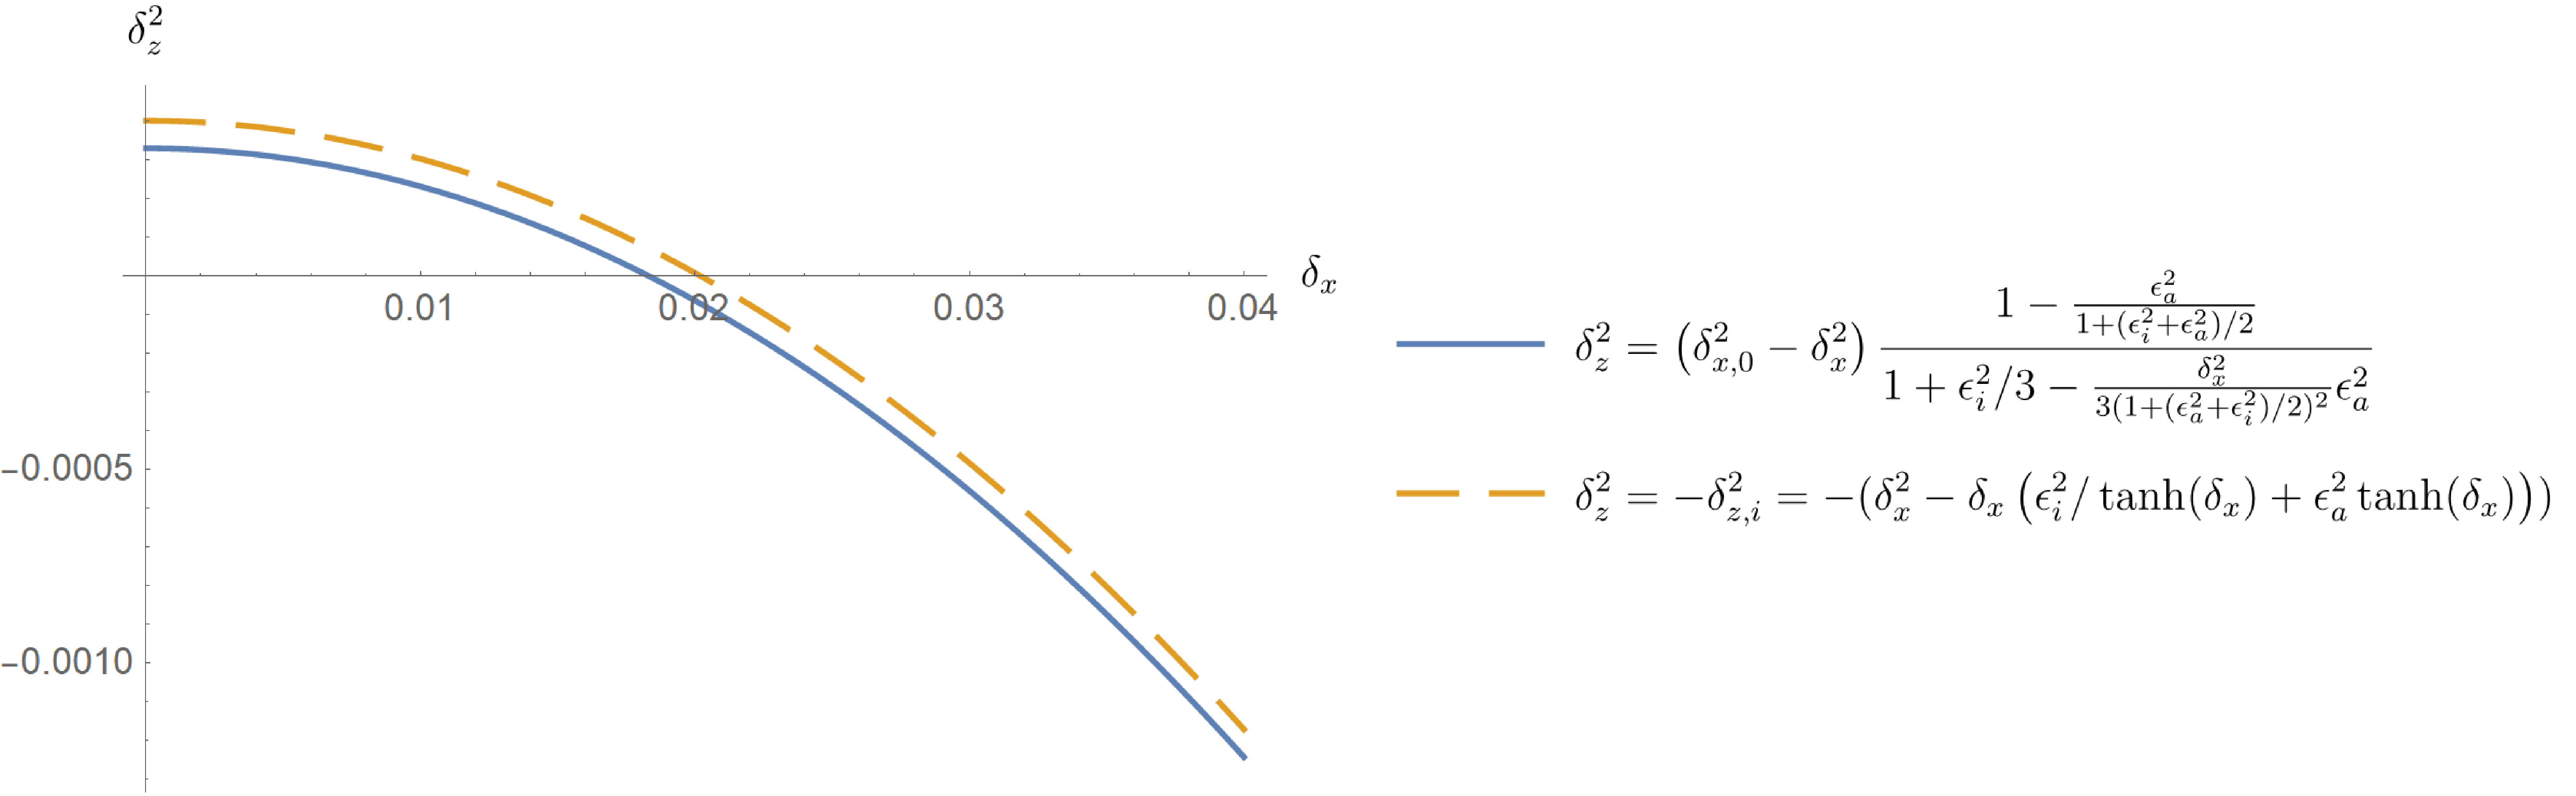
\includegraphics[width=0.9\linewidth]{FIGURES/dz2dx.png}
	}
\caption{Long waves: $\delta_z^2$ the square of the vertical wavenumber as a function of $\delta_x$ the horizontal wavenumber. The interval where $\delta_z^2$ is positive ($\delta_z$ real), for $\delta_x\le \delta_{x,0}$, corresponds to the barotropic mode while for $\delta_x\ge \delta_{x,0}$, $\delta_z^2$ is negative ($\delta_z$ purely imaginary) and this corresponds to the surface wave branch. The blue line is the accurate approximation given in \ref{deltazsurface} for long waves while the dashed orange curve corresponds to the approximation of surface waves given in \ref{longMSW}, this last approximation being more accurate for medium/short surface waves. The exact solution (not plotted), which can be numerically computed, is visually not distinguishable from the accurate blue curve.}
\label{dz2dx}
\end{figure}
\begin{figure}[h]
	\centerline{
		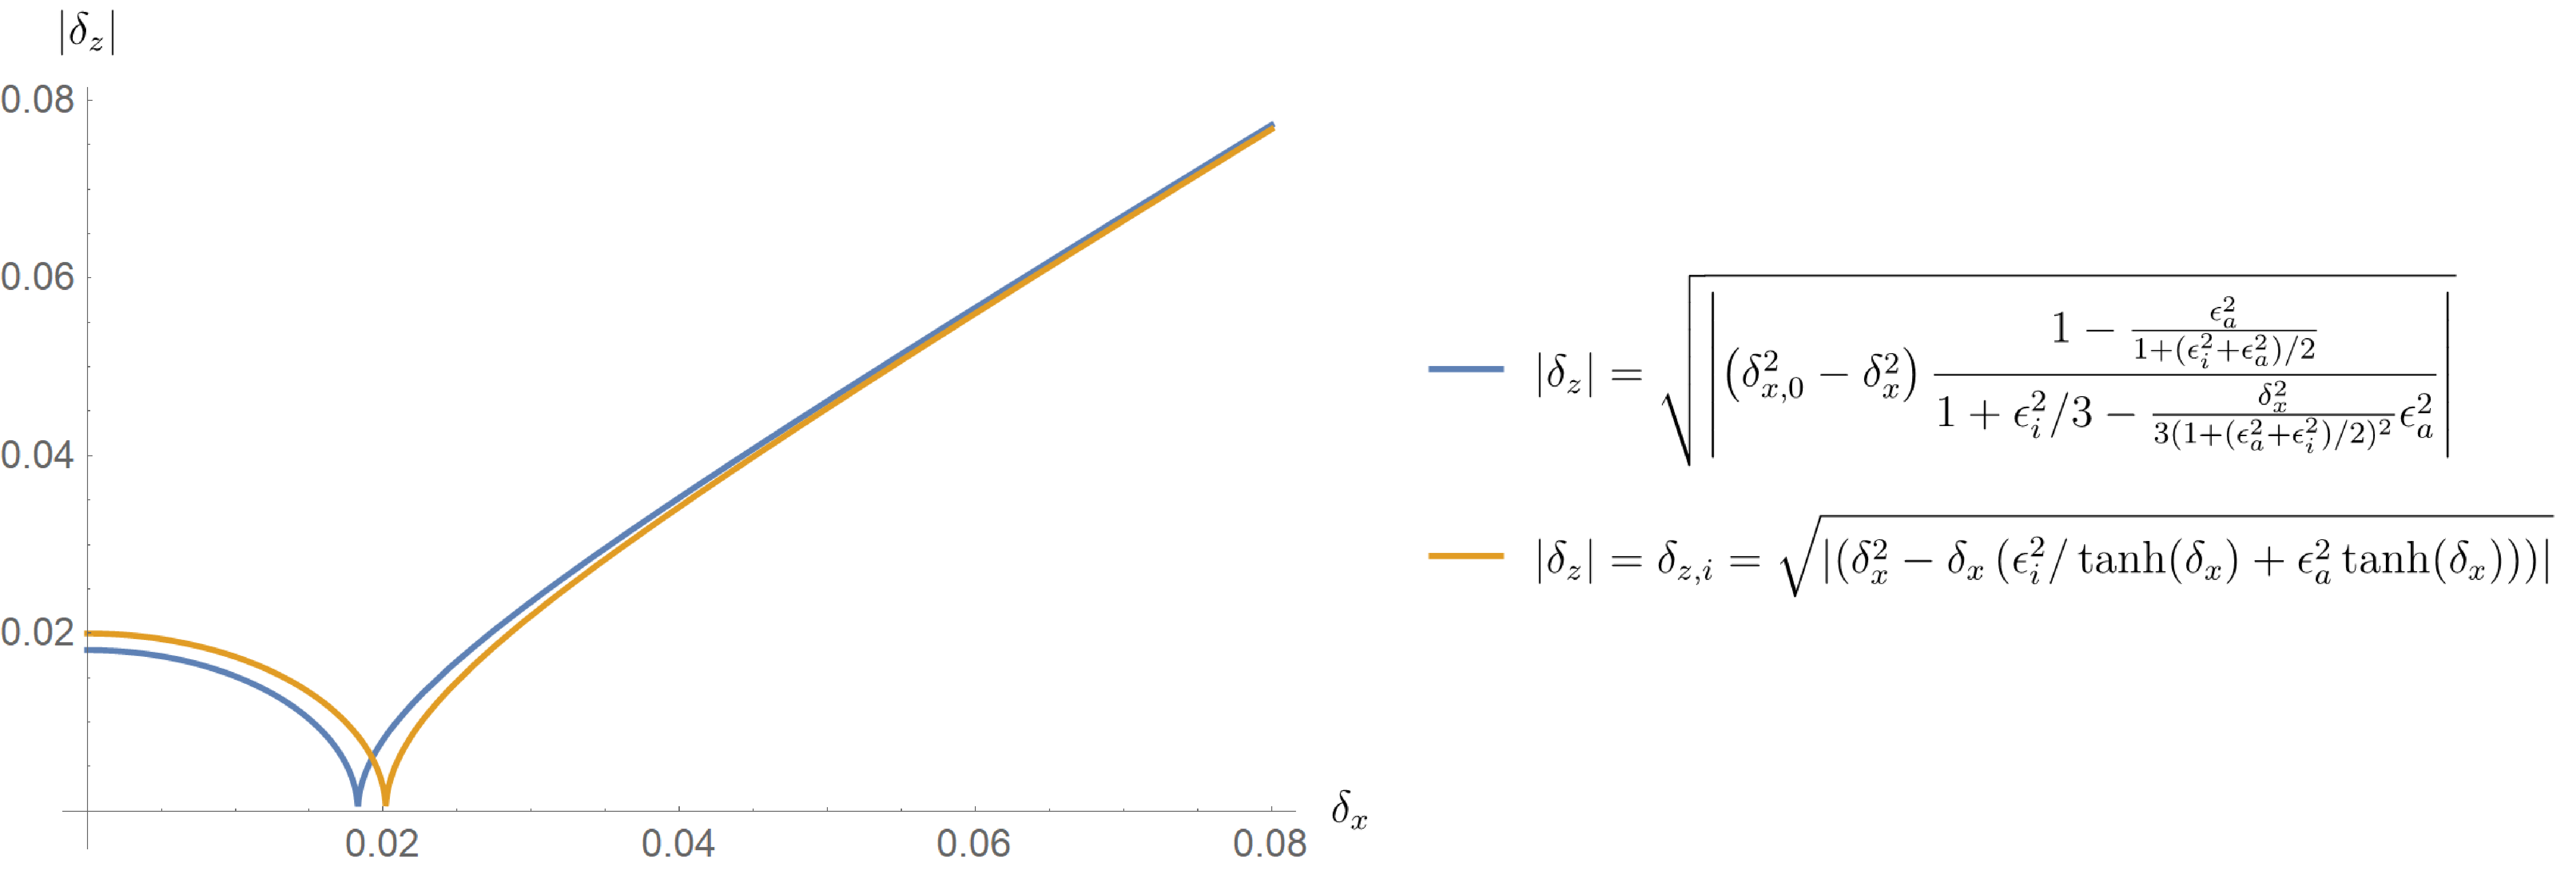
\includegraphics[width=0.9\linewidth]{FIGURES/dzdx.png}
	}
	\caption{Long waves: $|\delta_z|$ the modulus of the vertical wavenumber as a function of $\delta_x$ the horizontal wavenumber. The exact solution (not plotted), which can be numerically computed, is visually not distinguishable from the accurate blue curve. The vertical wavenumber of an incompressible and homogeneous ocean would correspond to the straight line $\delta_z=\delta_x$.}
	\label{dzdx}
\end{figure}
\\
%
%
Figure \oldref{omegadx} shows the values of the frequency $\omega$ as a function of the horizontal wavenumber $\delta_x$ according to different approximations. $\omega_{\mbox{\tiny Long Waves}}$ and $\omega_{\mbox{\tiny Medium Short Waves}}$ are computed by inserting the corresponding approximations \ref{deltazsurface} and \ref{longMSW} of $\delta_z$ in the boundary dispersion relation \ref{EqFullDisperb}. $\omega=\delta_x$ (resp. $\omega=\sqrt{\delta_x}$) is the classical long shallow water waves (resp. short non hydrostatic surface waves) approximation. $\omega=\sqrt{\delta_x \tanh(\delta_x)}$ is the frequency of an homogeneous and incompressible (non hydrostatic) ocean. Unsurprisingly, this last approximation is accurate over the full range of horizontal wavenumbers, even for the set of compressible stratified equations. Indeed, even if for long waves, $\delta_z$ is not directly linked to $\delta_x$ (in particular $\delta_z$ does not cancel for $\delta_x \approx 0$), $\delta_z$ remains small (less than $\epsilon_i$) and thus $\delta_z/\tan(\delta_z)$ is close to 1.
\begin{figure}[h]
	\centerline{
		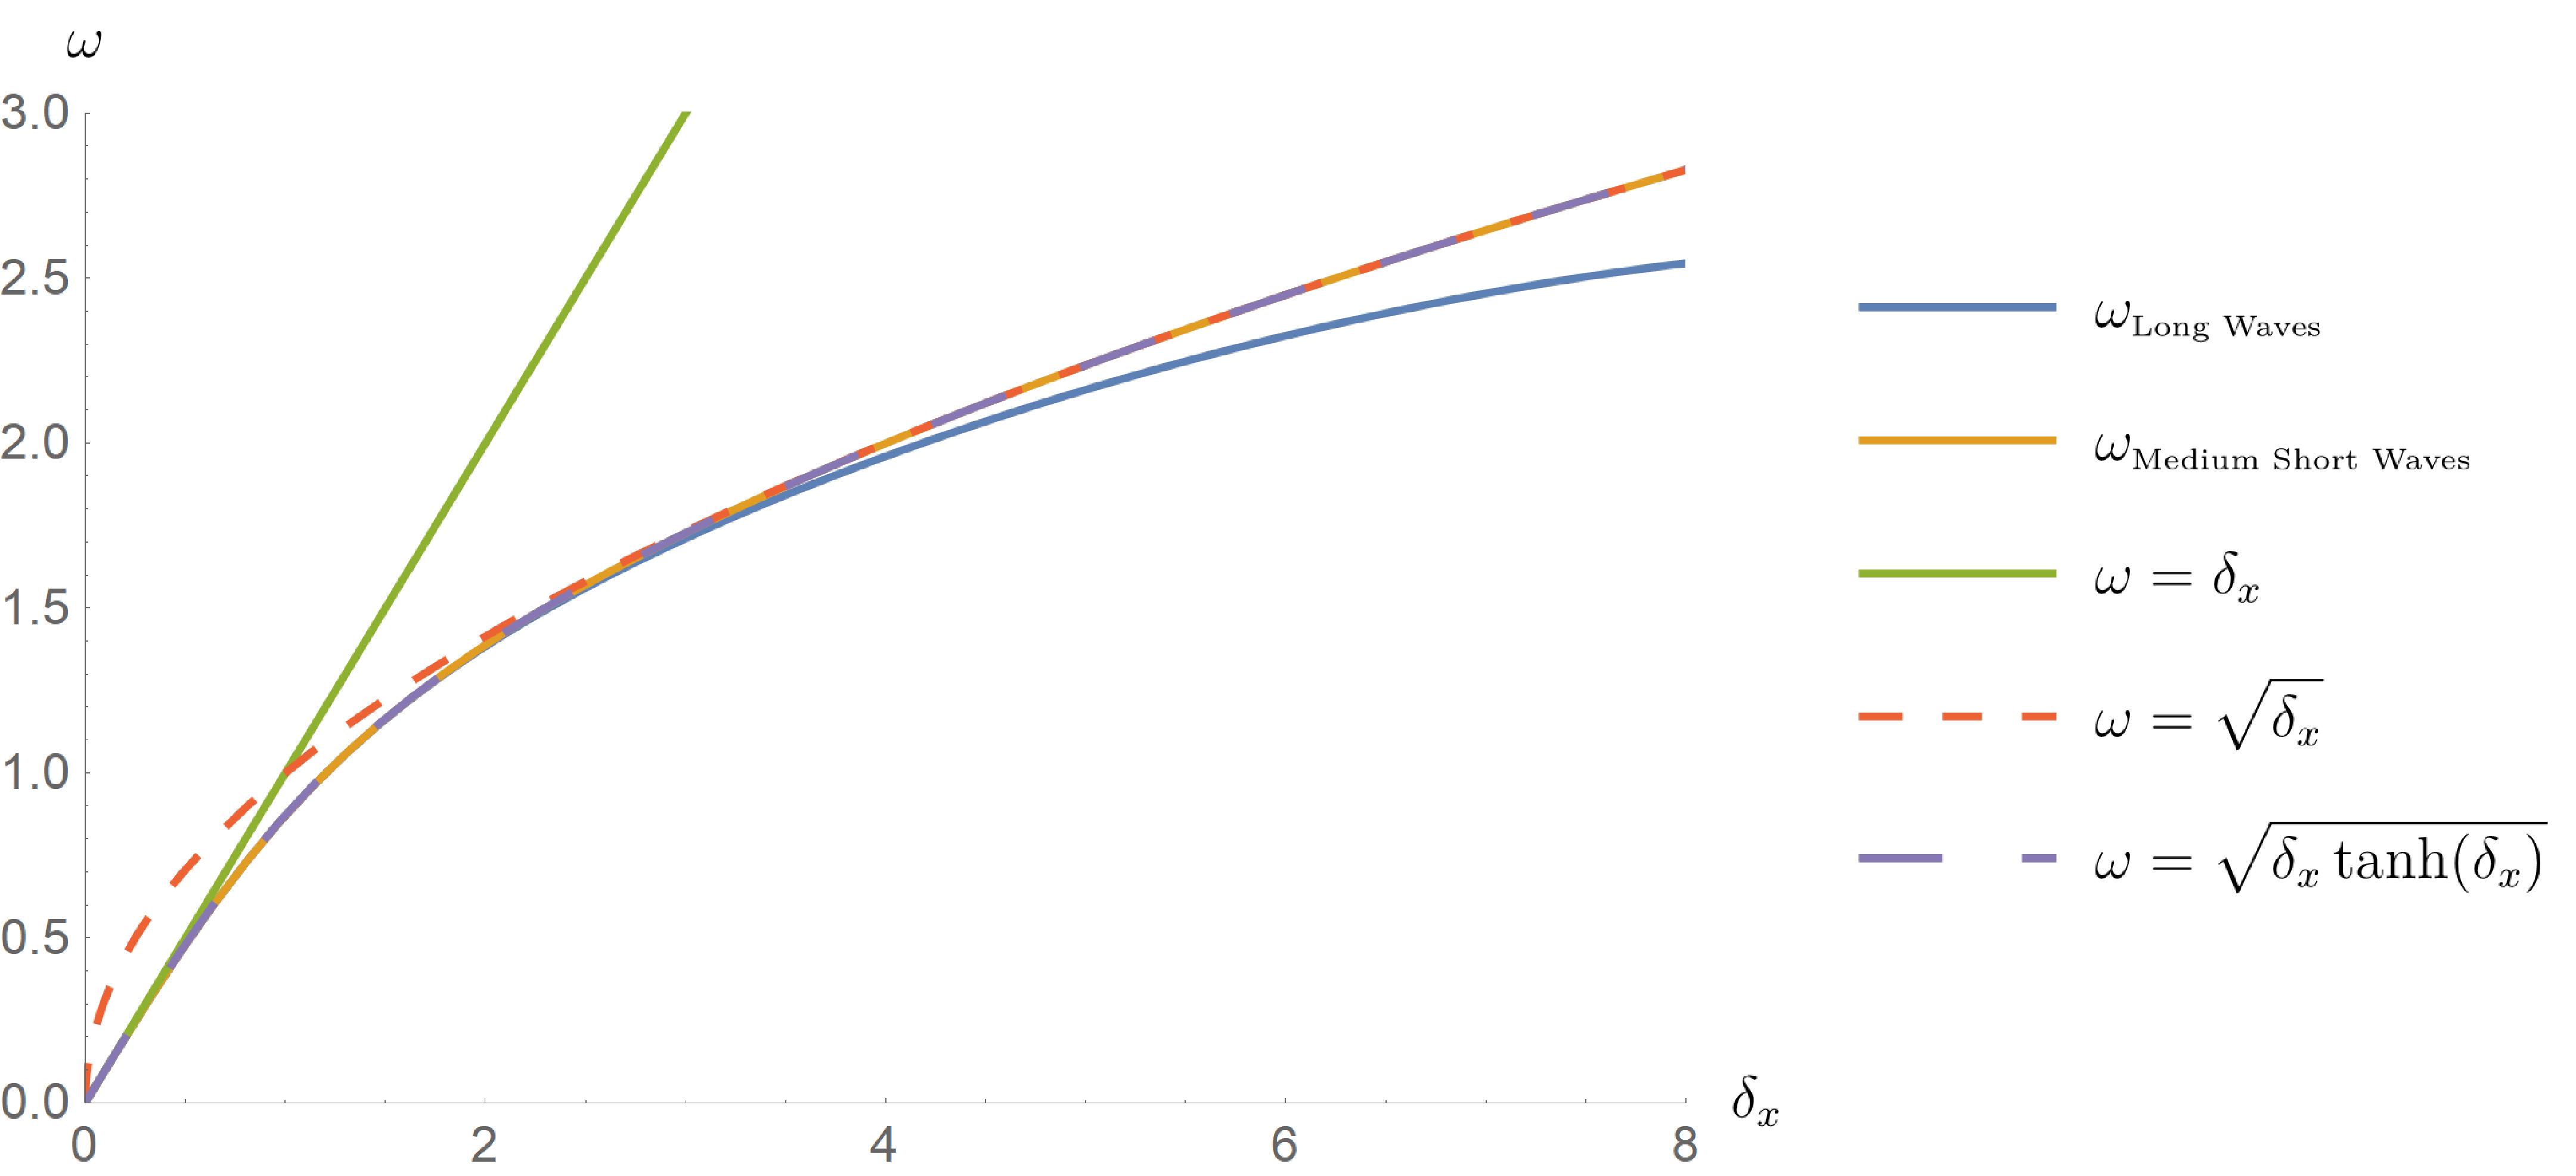
\includegraphics[width=0.9\linewidth]{FIGURES/omegadx.png}
	}
	\caption{Frequency $\omega$ as a function of $\delta_x$ the horizontal wavenumber for different approximations.}
	\label{omegadx}
\end{figure}


\textit{Orders of magnitudes:}\\
For the $4000m$-deep reference ocean (Table \oldref{TableParameters}), the horizontal length scale associated to the transformation of the MSW into the long MIM $(\lambda_{x,lmsw}=2\pi/(\delta_{x,lmsw}/4000))$ reaches $1367\ km$ against $62\ km$ for the same $10m$-deep ocean. When $\delta_x$ keeps on decreasing below $\delta_{x,lmsw}$, $\delta_z$ increases monotonically to a maximum value $\delta_{z,lmsw}(\delta_x=0)$. This vertical length scale reaches $1379\ km$ for the $4000m$-deep reference ocean and $62\ km$ for the same $10m$-deep ocean. The longer the horizontal length scale of the oscillation, the shorter the vertical length scale, and the weaker the stratification (vanishing $\epsilon_i$) the longer the horizontal length-scale $\lambda_{x,lmsw}$. This long MIM solution is a low-frequency oscillation of the ocean due to gravity and associated to the stratification of the ocean. It disappears when the stratification vanishes and the ocean can be assimilated to an homogeneous layer of water. It does persist in an incompressible ocean but is slightly modified by compressibility.

%\subsection{Close-to-singular MSW}
%
%The condition for propagation $(\displaystyle R^2(\delta_x,\delta_z)\le \frac{1}{4})$ derived in Section \ref{SubSectionFactoDisp} has so far been left out since for pulsations $\omega$ to remain real in the inner dispersion relation \ref{EqFullDispera}, it must necessarily be satisfied.  This condition is automatically satisfied for real horizontal and vertical wave-numbers but not necessarily for pure-imaginary vertical wave-numbers.\\
%A further question is to figure out if the resulting MSW wave solutions can or cannot approach and enter a region of the $(\delta_x,\ \delta_z,\ \omega)$ space where this condition is not satisfied. This would indeed lead to a pair of complex roots to \ref{solseq} and as a consequence to a wave solution diverging in time. Figure \ref{FigDelta} partially answers the question since it shows that the inner dispersion surface for pure-imaginary $\delta_z$ does not intersect the vertical (green) plane but remains tangent to it. We can show that the vertical component of the normal to the inner dispersion surface (i.e. $\partial$\ref{EqFullDisperai} $/\partial \omega$ ) vanishes for:
%\begin{equation}
%	   %\label{ParamAcousModes2}
%		\label{EqTurnPoints}
%		 \delta_x^2 - \delta_{z,i} ^2 
%		+\frac{(\epsilon_i^2+\epsilon_a^2)^2}{4}
%		-2 \epsilon_a^2 \omega^2 = 0
%\end{equation}
%	
%\begin{figure}[!h]
%	\centering		
%	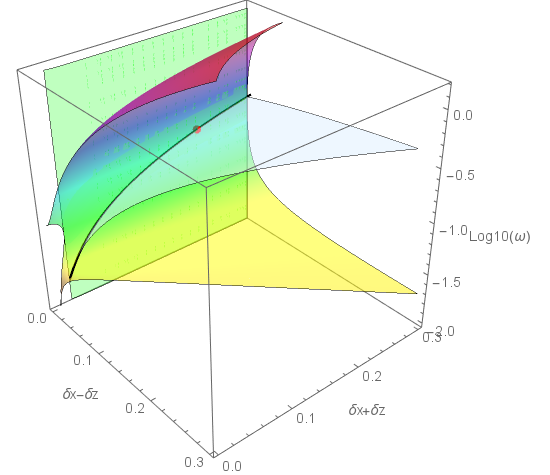
\includegraphics[width=0.5\linewidth]{FIGURES/Fig_Delta.png}
%	\caption{\textit{region of SMW close to instability (pure-imaginary vertical wave-number). Polychrome: inner dispersion surface. Light-blue: boundary dispersion surface. Light-green: vertical surface tangent to the inner dispersion surface. Red point: SMW solution close to instability. }}
%	\label{FigDelta}
%\end{figure}
%
%
%This set of points of the inner dispersion surface satisfies $\displaystyle R^2(\delta_x,i \delta_{z,i})= \frac{1}{4}$ and, as a consequence,
%$\omega^2=\omega_a^2/2$. They correspond to the black line on Figure \ref{FigDelta}. This line separates the inner dispersion surface in two parts: the upper acoustic region $(\omega^2\approx\omega_a^2)$ closer to the MAM branch and the lower region $(\omega^2\approx\omega_i^2)$ closer to the MIM region.\\
%If solutions to \ref{EqTurnPoints} and \ref{EqFullDisperai} can be found, at least one MSW wave intersects this line of points in phase-space. Such an intersection exists if there exist at least one point belonging to the boundary dispersion surface given by \ref{EqFullDisperb} or equivalently if the system of equations \ref{EqTurnPoints}, \ref{EqFullDisperai} and \ref{EqFullDisperb} has a solution. Only one single point satisfies this system, it is indicated by a large red dot on \ref{FigDelta}. Its horizontal and vertical wave-numbers can be expressed as functions of its pulsation:
%\begin{subequations}
%	\begin{alignat}{2}	
%	   \label{ParamSolDelta}
%	   &\delta_{z,i}(\omega) && =\frac{1}{2} 
%	   \sqrt{(\epsilon_i^2+\epsilon_a^2)^2 
%	   - 8 \epsilon_a^2 \omega^2
%	   + 4 \frac{\epsilon_a^2}{\epsilon_i^2} \omega^4}\\[3mm]
%	   &\delta_x(\omega) &&=\omega
%	   \sqrt{\frac{\epsilon_a^2+\epsilon_i^2}{2}
%	   +\delta_{z,i}(\omega)\ coth(\delta_{z,i}(\omega))}
%	\end{alignat}
%\end{subequations}
%The pulsation $\omega$ must then be a solution of the (transdental) equation inherited from the inner dispersion relation \ref{EqFullDisperai}:
%\begin{subequations}
%	\begin{alignat}{2}	
%	   \label{ParamSolDelta2}
% 		\delta_x^2(\omega)-\delta_{z,i}^2(\omega) 
% 		-\epsilon_i^2\ \frac{\delta_x^2(\omega)}
% 			{\omega^2}-\epsilon_a^2\omega^2
% 		+\frac{\epsilon_a^2+\epsilon_i^2}{4} = 0
%	\end{alignat}
%\end{subequations}
%For the parameters $\epsilon_i$ and $\epsilon_a$ given in Table \ref{TableParameters}, this latter equation has only one solution for $\omega^*$ satisfying the system of equations \ref{EqTurnPoints}, \ref{EqFullDisperai} and \ref{EqFullDisperb}. It can be evaluated numerically:
%\begin{equation}
%	\omega_* \approx 0.154
%\end{equation}
%Orders of magnitude of the wave-numbers $(\delta_{x,*},\ \delta_{z,*})$ and pulsations $(\omega_*)$ are given in Table \ref{TableOrdersMag}. The resulting wave solution is a MSW wave that satisfies $R^2(\delta_{x,*},\ \delta_{z,*})=1/4$. Graphically this means that the solution point (in red) belongs to the line of points with horizontal normal vector or vanishing vertical gradient with respect to $\omega$. Dynamically, this means that the corresponding wave solution is "on the edge" and that for a small variation of the wave-number, of the pulsation or one the parameters it may enters in the region of unstable waves satisfying $R^2>1/4$. \\
%Other reference parameters given in Table \ref{TableParameters} remaining constant, Table \ref{TableOrdersMag} shows that when changing the depth of the reference ocean (4000 m) to only 10 m, the (normalized) pulsation $\omega_*$ remains quasi-constant and, as a consequence, the pulsation $\Omega_*$ varies approximately with $0.154 \sqrt{g/H}$ in this range of parameters ($\Omega_*$ decreases thus from $12\ mn$ to only $41.3\ s$).


\subsection{Summary: waves solutions in a bounded ocean}
Table \oldref{TableWavesolutions_boundedmodified} summarizes the main results of this paper. The approximation for the different kind of waves (acoustic, gravity and surface waves/modes) are indicated in their dimensional form. For sake of readability, some of the relations given in Table \oldref{TableWavesolutions_boundedmodified} are lower order version of what has been proved previously. Most of the time, its corresponds to taking into account  the first-order correction terms only, in comparison to usual dispersion relation introduced in Table \oldref{TableWave solutions}. In that case, a red link to the higher approximation is given.
\begin{table}[!h]
	\centerline{
			\setlength{\extrarowheight}{30pt}
		\rotatebox{90}{
		\begin{tabular} {p{3.0cm}|p{8.6cm}|p{8cm}}
			Waves &  Frequency $(\Omega)$ & Vertical wavenumber $k_z$\\\hline
\begin{minipage}{3cm}
Modified Acoustic Modes (MAM)\\
$\small k_{z,m}=\frac{1}{H}(\pi/2+m\pi), m\ge 0$\\
\ref{SubSectionGraphicMAW}
\end{minipage}&
			$\displaystyle \Omega_{mam}^2=c_s^2(k_x^2+k_z^2)
			\left[
			1-\frac{g}{Hc_s^2}\frac{k_x^2-k_{z,m}^2}{(k_x^2+k_{z,m}^2)^2}+\frac{N^2}{gH}\frac{1}{k_x^2+k_{z,m}^2}
			\right]$&
			$\displaystyle
			k_{z,m}
			\left[
			1-\frac{g}{Hc_s^2}\frac{k_x^2-k_{z,m}^2}{2(k_x^2+k_{z,m}^2)k_{z,m}^2}
			+\frac{N^2}{2gH^2}\frac{1}{k_{z,m}^3}
			\right]
			$\quad {\color{red}\ref{ParamallMAM1}}	
			\\[8mm] \hline
\begin{minipage}{3cm}
Modified Internal Modes (MIM)\\
$k_{z,n}=\frac{1}{H}(n\pi), m\ge 1$\\
\ref{SubSectionGraphicMIW}
\end{minipage}
& $\displaystyle \Omega_{mim}^2=\frac{N^2 k_x^2}{k_x^2+k_{z,n}^2}
			\left[
			1-2\frac{N^2}{gH}\frac{k_{z,n}^2}{(k_x^2+k_{z,n}^2)^2}
			\right]
			$
			&
			$\displaystyle
			k_{z,n}
			\left[
			1+\frac{N^2}{gH}
			\frac{1}{k_x^2+k_{z,n}^2}
			+\left(\frac{N^2}{gH}\right)^3
\frac{(k_x^2-k_{z,n}^2)}{(k_x^2+k_{z,n}^2)^3}
			\right]
			$		\\[8mm] \hline
\begin{minipage}{3cm}
Barotropic mode\\
$k_x\le k_{x,0}\approx \frac{N^2}{g}$\\
\ref{SubSectionLongWavesrealdz}
\end{minipage}&
$\Omega^2 = gHk_x^2 \left[
1
-\frac{1}{6}\left(
\epsilon_i^2+3\epsilon_a^2
\right)
\right]$\qquad {\color{red}\ref{eqomegalongwavereal}}&
$\displaystyle \sqrt{k_{x,0}^2-k_x^2}$
\qquad
{\color{red}\ref{deltazsurface}}
\\[8mm] \hline
\begin{minipage}{3cm}
Long\\
surface waves\\
$k_x\ge k_{x,0}\approx \frac{N^2}{g}$\\
\ref{SubSectionLongWavesrealdz}
\end{minipage}
&$\Omega^2 = gHk_x^2 \left[
1
-\frac{1}{6}\left(
\epsilon_i^2+3\epsilon_a^2
\right)
\right]$\qquad {\color{red}\ref{eqomegalongwavereal}}&
$\displaystyle i\sqrt{k_x^2-k_{x,0}^2}$
\qquad
{\color{red}\ref{deltazsurface}}
\\[8mm] \hline
\begin{minipage}{3cm}
Medium and short\\
surface waves\\
$k_x\ge k_{x,0}\approx \frac{N^2}{g}$
\\
\ref{SubSectionGraphicMSW}
\end{minipage}
&
$\displaystyle
\Omega^2=
gk_x\tanh(Hk_x)$
\qquad
{\color{red}\ref{eqomegasurfacewaves}}
&
$\displaystyle i k_x \sqrt{1-\frac{1}{k_x}\left(
\frac{N^2}{g\tanh(Hk_x)}
+
\frac{g}{c_s^2}\tanh(Hk_x)
\right)}$
	\end{tabular}}}
	\caption{{\color{red}corriger legende ...}Compressibility and stratification induced modifications to the usual dispersion relations given in table \ref{TableWave solutions}. $\Omega$ is wave angular frequency, $k_x$ and $k_z$ are the wavenumbers, $g$ is the acceleration of gravity, $N$ a reference Brunt-V\"ais\"al\"a frequency and $c_s$ the speed of sound. $D_0$ is the background density vertical scale and is given by $1/D_0=N^2/g+g/c_s^2$}
	\label{TableWavesolutions_boundedmodified}
\end{table}
\newpage
{\color{red}FIN MODIFS LAURENT}
%%%%%%%%%%%%%%%%%%%%%%%%%%%
% Table order of magnitude
%%%%%%%%%%%%%%%%%%%%%%%%%%%
\begin{table}[h]
	%\centerline{
	\begin{tabular}{l|l|l|l|l}
		& \textit{Notation}   & \textit{Reference} & \textit{10-m-deep} & \textit{$N=10^{-2}\ s^{-1}$}\\\hline
		Parameters & $\epsilon_a$ &
		$0.13$ &
		$6.6\  10^{-3}$ & $0.13$\\
		& $\epsilon_i$ &
		$2.0\ 10^{-2}$ &
		$1.0\ 10^{-3}$ & $0.20$\\\hline
		\specialrule{0pt}{2pt}{0pt}
		Acoustic cut-off&$2\pi \sqrt{H/g} /\omega_{c,a}$ & $30\ mn$ & $30\ mn$ & $9.6\ mn$\\\hline
		\specialrule{0pt}{2pt}{0pt}
		Internal cut-off& $2\pi \sqrt{H/g} /\omega_{c,i}$& $1.7\ h$ & $1.7\ h$ & $10.5\ mn$\\\hline
		\specialrule{0pt}{2pt}{0pt}
		LMIM-LMSW cut-off & $2\pi H/\delta_{x,0}$& $1367\ km$ & $1000\ km$ & $123\ km$\\
		& $2\pi \sqrt{H/g} \omega_{x,0}$ & $1.9\ h$ & $1.7\ h$ & $10.5\ mn$\\\hline
		\specialrule{0pt}{2pt}{0pt}
		LMIM-$\delta_z(0)$ & $2\pi H/\delta_{z,0}$& $1379\ km$ & $62\ km$& $125\ km$\\
		& $2\pi \sqrt{H/g} \omega_{z,0}$ & $\infty$& $\infty$ & $\infty$\\ \hline
		\specialrule{0pt}{2pt}{0pt}
		MSW-neutral point & $2\pi H/\delta_{x,*}$& $161\ km$ & $407\ m$ & $123\ km$\\
		&$2\pi H/\delta_{z,*}$ & $164\ km$ & $407\ m$&$2148\ km$\\
		&$2\pi \sqrt{H/g} \omega_{*}$ &$12\ mn$&$41.3\ s$&$10.5\ mn$\\
	\end{tabular}
	%}
	\caption{orders of magnitude of various scales. Notations refer to non-dimensional variables whereas orders of magnitude are given for dimensional quantities. Parameters for the "\textit{Reference}" ocean are given in Table \ref{TableParameters}. "\textit{10-m-deep}" ocean is a  10-m-deep \textit{Reference} ocean and "$N=10^{-2}\ s^{-1}$" refers to a \textit{"Reference"} ocean with $N=10^{-2}\ s^{-1}$.} 
	\label{TableOrdersMag}
\end{table}
%%%%%%%%%%%%%%%%%%%%%%%%%%%%%%%%%%%%%%%%%%%%%%%%%%%%%%%%%%%%%%%%%%%%%%%%%%%
\section{Discussion, conclusion}
\label{SectionDiscussion}
%%%%%%%%%%%%%%%%%%%%%%%%%%%%%%%%%%%%%%%%%%%%%%%%%%%%%%%%%%%%%%%%%%%%%%%%%%%
The Lagrangian model of \cite{dukowicz_2013} for acoustic, gravity and surface waves, based on two dispersion relations, is revisited in the present study within a fully Eulerian approach. The latter is not physically more coherent but its derivation and analysis are simpler. Acoustic and internal wave rays propagating in an unbounded ocean are first evaluated with a single dispersion equation. Smith's acoustic modes \citep{smith_2015} are recovered and both short and long-wave approximations are proposed. Then, well-known internal modes and surface waves (edge waves) are revisited in a compressible, stratified, free-surface ocean. Long surface waves are analyzed and their classification as barotropic modes questioned. This work complements efforts made by Dukowicz to provide a coherent and complete framework for the description of geophysical waves, integrating new wave solutions and clarifying the description of key phase-space regions such as long waves.

A graphical analysis is proposed, using the $(\delta_x,\ \delta_z,\ \omega)$ phase-space to classify ocean waves and modes: intersections of the inner and boundary dispersion surfaces are localized numerically and used as references to derive wave approximations. This original investigation in phase-space, associated with Taylor developments with respect to small compressibility and stratification parameters, provides an adapted approach to circumvent the nonlinear and transcendental characters of the boundary dispersion relation and the (high) fourth-order dependency in frequency $\omega$ of the inner dispersion relation. In $(\delta_x,\ \delta_z,\ \omega)$ phase-space, the inner dispersion surface is decomposed into three distinct branches with a one-to-one correspondence along the $\omega$ axis. At high frequency, the \textit{acoustic branch} is well described by the simple factorizing function $\omega_a$ and is bounded for vanishing $(\delta_x,\ \delta_z)$ by the acoustic cut-off frequency $(\omega_{MAM,-})$. Acoustic waves propagating in the ocean as in an unbounded medium (MAW) belongs to this branch together with acoustic modes modified by gravity (MAM) which can be found at the intersection of this acoustic branch with the dispersion boundary surface given by the transcendental relation \ref{EqFullDisperb}.

At low frequency (long waves), the \textit{internal gravity branch} of the inner dispersion surface is in turn well approximated by the internal factorizing function $(\omega_i)$. The frequency of internal waves in this branch is bounded by the internal parameter $\epsilon_i$ (the cut-off frequency is $N$, the Brunt-Väisälä frequency). Internal gravity rays belong to this surface. At the intersection of the lower-frequency gravity branch with the \textit{boundary dispersion surface} are found internal gravity modes (MIM).

Compressibility perturbations to MIM and gravity perturbations to MAM are shown to be high-order perturbations in small parameters $\epsilon_i$ and $\epsilon_a$. These wave-modes are well-separated graphically and analytically. They are thus well approximated respectively by the stratification and acoustic factorizing functions $\omega_i$ and $\omega_a$. The situation is somehow different for MSW. The wave solution in this case is a linear combination of real roots $(\omega_\pm)$, but these two roots might not be well-separated for waves with purely imaginary vertical wavenumbers. A consequence is that unlike for real vertical wavenumbers, the contributions of acoustic and stratification factorizing functions $\omega_a$ and $\omega_i$ cannot be meaningfully separated.

Well-know relations for internal wave-rays or acoustic waves in an unbounded ocean and for internal-gravity or acoustic wave-modes in a bounded ocean are recovered. Lower-order perturbations due to stratification and gravity ($\epsilon_i$) and to compressibility ($\epsilon_a$) are proposed for each type of waves. Acoustic Lamb-waves are examined as a particular case: they are solutions of the proposed (first-order) wave-model only under an additional "rigid-lid" assumption.\\

Between these upper and lower branches of the inner dispersion surface, waves can propagate with middle-range frequencies only if their vertical wavenumber is a purely imaginary complex. The intersection with the \textit{boundary dispersion surface} hosts surface waves (MSW) which can be "modified" by compressibility and stratification. The medium-range branch is indeed "folded" by both compressibility and stratification. In both cases, the surface is bounded: an upper bound for vanishing wavenumbers due to acoustic cut-off; and a lower bound for high frequencies due to Brunt-Väisälä cut-off. When frequency is increased from very low values, MSW intersections can change from surface waves modified by stratification to surface waves modified by compressibility. In the transition region, the two wave solutions merge into a single "neutral" solution at the limit where frequency is purely imaginary.
%%Three branches of surface solutions have been identified: one for pure-imaginary vertical wave-numbers $(\delta_z)$ includes MSW solutions, the remaining two (this time for real $\delta_z$) includes MAW, MIW, MAM and MIM. The latter two branches have been shown to be well-separated in $(\delta_x,\ \delta_z,\ \omega)$ space. This confirms, if necessary, that surface, acoustic and internal solutions belong to different branches of dispersion surfaces. They are based on different propagating mechanisms. \\
%%These wave solutions have been first identified graphically in the $(\delta_x,\ \delta_z,\ \omega)$ phase-space. The large-pulsation branch is

In the long-wave limit, a modified "n=0" gravity mode (MIM-0) exists only in a stratified ocean. It can be associated with a low-frequency branch of the real-$\delta_z$ inner dispersion surface. Therefore, it cannot be the asymptotic limit of shorter swell-like MSW branch. Usual approximations for long surface waves ($\delta_z=\delta_x$ and $\omega=\delta_x$) can be recovered from our results in two ways. It can either be introduced as a long-wave approximation of MSW for an homogeneous (non-stratified) ocean or as a long-wave approximation of mode-0 MIM. In the latter case, a vanishing vertical wavenumber is recovered only for $\epsilon_i=\epsilon_a=0$.
%For small horizontal wave-number, the wave solution can be viewed as a (long) \textit{barotropic mode} $(n=0)$ since it is on the same inner dispersion branch as MIM which are solutions for $n>0$.

MSW are thus primarily edge waves: the free-surface anomaly is one way or the other translated into a pressure anomaly by gravity; wave propagation is then achieved by a simple compensation mechanism based on the conservation of mass and momentum. If the ocean is homogeneous and incompressible, the pressure is a harmonic function and horizontal and vertical length-scales are equal $(\delta_x=\delta_z)$. With compressibility and stratification, horizontal and vertical wavenumbers becomes different (Sec. \ref{subsubsectioniR}). If $\delta_x$ decreases, $\delta_z$ decreases even faster and vertical MSW variations become very small. If $\delta_x$ further decreases, $\delta_z$ finally vanishes for small but finite $\delta_x$. If the horizontal wavenumber keeps on decreasing, a surface wave can only propagate as a mode-0 MIM. In this case, the vertical wavenumber must increase again due to a stratification barrier: the stronger the stratification, the shallower the penetration depth of surface waves.\\

In a stratified ocean (whether compressible or not), long surface waves (LMSW in the vicinity of the origin in phase-space) cannot propagate and are replaced by (mode-0) MIM solutions. The longest surface wave that can propagate is barotropic (depth-independent): its horizontal wave-number is $\delta_{x,lmsw}$ and its vertical wave-number is zero. When the stratification weakens, $\delta_{x,lmsw}$ tends toward 0 and the resulting long waves approaches LSW (with $\sqrt{g H}$ phase and group velocity and $\delta_x=\delta_z$).
Propagation in an homogeneous ocean can be studied with the present model by setting to zero the stratification parameter $\epsilon_i$ together with the last (advective) term on the right-hand-side of the inner dispersion relation \ref{EqFullDispera}: $-(\epsilon_i^2+\epsilon_a^2)^2/4$. 

Further inspection of MSW waves has shown that there exists a particular triplet of properties $(\delta_x,\ \delta_z,\ \omega)$ for which the pair of real roots \ref{solseq} merges and the discriminant of the second-order polynomial equation in the pulsation vanishes. This double root is located in the region where the inner dispersion surface is vertical and contributions due to compressibility and stratification are smaller. This MSW solution is very peculiar in the sense that it is located at the edge of the region of $(\delta_x,\ \delta_z,\ \omega)$ phase-space where wave solutions are divergent as time goes on. Ocean waves originating in this region of phase space might have singular behaviour.\\
\subsection*{Acknowledgements}
This study has received support from a consortium of French research agencies, as part of CROCO's development project (GdR CROCO). Laurent Debreu has received funding from the European Union's Horizon 2020 research and innovation program under grant agreement No. 821926 (IMMERSE). Eric Blayo, Emilie Duval and Laurent Debreu have received funding from the SHOM/DGA under grant agreement No 18CP03.
\bibliographystyle{apalike}
\bibliography{paperagwaves}
%%%%%%%%%%%%%%%%%%%%%%%%%%%%%%%%%%%%%%%%%%%%%%%%%%%%%%%%%%%%%%%%%%%%%%%%%%%%%
\appendix
\section{$\delta_z$ real or purely imaginary}
\label{kzreal}
In this section, we prove that under the condition of smallness of parameters $\epsilon_i$ and $\epsilon_a$, $\delta_z$ is either real or pure imaginary and thus that the frequency $\omega$ is real.\\
The eigenvalue problem \ref{EqDimF} and the surface boundary condition \ref{EqDimFb} are rewritten in non-dimensional form as:
\begin{align}
G''(s)
+
\delta_z^2
G(s)&=0 \label{sturm1}\\
G(1)&=1 \label{sturm2}\\
G(0)&=0 \label{sturm3}
\end{align}
\begin{equation}
G'(1)+\left(
\frac{\epsilon_i^2+\epsilon_a^2}{2}-\frac{\delta_x^2}{\omega^2}
\right) G(1)=0
\label{eqnormal}
\end{equation}
where $\displaystyle s=\frac{z+H}{H}$, $G(s(z))=F(z)$ and $\displaystyle \epsilon_i^2=\frac{N^2H}{g}, \epsilon_a^2=\frac{gH}{c_s^2},\delta_x=k_xH,\delta_z=k_zH,\omega=\Omega\sqrt{\frac{H}{g}}$.\\
$\delta_z$ is linked to $\delta_x$ and $\omega$ by the inner dispersion relation
\begin{equation}
\delta_z^2=\left(\delta_x^2\frac{\epsilon_i^2-\omega^2}{\omega^2}
+\epsilon_a^2\omega^2-\frac{(\epsilon_i^2+\epsilon_a^2)^2}{4}\right)
\label{innerannex}
\end{equation}
Multiplying \ref{sturm1} by $\overline{G(s)}$ and integrating over $[0,1]$ we get:
\[
\int_0^1G''(s)\overline{G(s)}{\rm d}s+\delta_z^2\int_0^1|G(s)|^2{\rm d}s=0
\]
Integration by parts leads to:
\[
-\int_0^1|G'(s)|^2{\rm d}s+\delta_z^2\int_0^1|G(s)|^2{\rm d}s+G'(1)\overline{G(1)}-G'(0)\overline{G(0)}=0
\]
and using \ref{sturm2}, \ref{sturm3}, \ref{eqnormal}
\[
\delta_z^2 \int_0^1|G(s)|^2{\rm d}s+\left(\frac{\delta_x^2}{\omega^2}-
\frac{\epsilon_i^2+\epsilon_a^2}{2}
\right)=\int_0^1|G'(s)|^2{\rm d}s
\]
Using the Poincar\'e inequality $\displaystyle \int_0^1|G(s)|^2{\rm d}s\le \int_{0}^1|G'(s)|^2{\rm d}s$ and $\displaystyle 1=|G(1)|^2 \le \int_{0}^1|G'(s)|^2 {\rm d}s$, we obtain:
\begin{equation}
\delta_z^2 \mu + \left(
\frac{\delta_x^2}{\omega^2}-\frac{\epsilon_i^2+\epsilon_a^2}{2}
\right)
\nu = 1
\label{sturm4}
\end{equation}
with $0\le \mu \le 1$ and $0\le \nu \le 1$.\\
Taking the imaginary part of \ref{sturm4} and using \ref{innerannex}
\[
\mu \left( \epsilon_a^2 \Im[\omega^2] +\delta_x^2 \epsilon_i^2 \Im[1/\omega^2]\right)+\nu \delta_x^2\Im[1/\omega^2]=0
\]
or, using $\Im[1/\omega^2]=-\Im[\omega^2]/|\omega|^4$,
\begin{equation}
\Im[\omega^2]\left(\mu \left(\epsilon_a^2 -\epsilon_i^2 \frac{\delta_x^2}{|\omega|^4} \right) -\nu \frac{\delta_x^2}{|\omega|^4} \right)=0
\label{constraint1}
\end{equation}
Let us assume that $\omega$ is neither real or pure imaginary. This implies $\Im[\omega^2] \ne 0$ and \ref{constraint1} leads to:
\begin{equation}
\mu\left(\epsilon_a^2\frac{|\omega|^4}{\delta_x^2} -\epsilon_i^2\right)-\nu=0
\label{eqmunu1}
\end{equation}
We will show below that, in this case, solutions can exist only for non physical values of $\epsilon_i, \epsilon_a$ satisfying $\max(\epsilon_i,\epsilon_a) > \sqrt{2}$.\\
Taking the real part of \ref{sturm4}
\[
\mu \left(-\delta_x^2+\delta_x^2\epsilon_i^2\Re[1/\omega^2]-\frac{(\epsilon_i^2+\epsilon_a^2)^2}{4}+\epsilon_a^2 \Re[\omega^2]\right)
+\nu \left(
\delta_x^2 \Re[\frac{1}{\omega^2}]-\frac{\epsilon_i^2+\epsilon_a^2}{2}
\right)=1
\]
or, using $\Re[1/\omega^2]=\Re[\omega^2]/|\omega|^4$,
\[
\mu \left(-\delta_x^2-\frac{(\epsilon_i^2+\epsilon_a^2)^2}{4}+(\frac{\delta_x^2\epsilon_i^2}{|\omega|^4}+\epsilon_a^2 )\Re[\omega^2]\right)
+\nu \left(
\frac{\delta_x^2}{|\omega|^4} \Re[\omega^2]-\frac{\epsilon_i^2+\epsilon_a^2}{2}
\right)=1.
\]
\ref{eqmunu1} allows to simplify in:
\begin{equation}
\mu \left(-\delta_x^2-\frac{(\epsilon_i^2+\epsilon_a^2)^2}{4}+2\epsilon_a^2\Re[\omega^2] \right)
-\nu \left(
\frac{\epsilon_i^2+\epsilon_a^2}{2}
\right)=1
\label{eqmunu2}
\end{equation}
Eqs \ref{eqmunu1} and \ref{eqmunu2} can be summarized in 
\begin{equation}
\begin{array}{l}
\alpha \mu  - \beta \nu = 1\\
\gamma \mu - \nu=0
\end{array}
\label{eqmunu}
\end{equation}
with
\[
\alpha= -\delta_x^2-\frac{(\epsilon_i^2+\epsilon_a^2)^2}{4}+2\epsilon_a^2\Re[\omega^2], \beta = \frac{\epsilon_i^2+\epsilon_a^2}{2}, \gamma =  \epsilon_a^2\frac{|\omega|^4}{\delta_x^2} -\epsilon_i^2
\]
Using $\beta > 0$, it is easy to check that \ref{eqmunu} has solutions $(\mu,\nu)$ positive and with magnitude less than one only if
\[
\gamma>1 \mbox{ and }\alpha > (1 + \beta ) \gamma
\]
or
\[
0\le \gamma\le 1 \mbox{ and }\alpha \ge 1 + \beta \gamma
\]
The conditions above immediately exclude the cases $\epsilon_a=0$ (which leads to $\gamma < 0$ ) and $\Re[\omega^2] \le 0$ (which leads to $\alpha <  0$ ). They will not be considered below.
\begin{itemize}
	\item First case: $0\le \gamma \le 1$\\
	This implies:
	\begin{equation}
	|\omega|^4 \le \frac{\delta_x^2}{\epsilon_a^2}(1+\epsilon_i^2)
	\label{maj1}
	\end{equation}
	$\alpha \ge 1 + \beta \gamma$ writes:
	\[
	\Re[\omega^2] \ge  \frac{1}{2\epsilon_a^2}\left[
	1+\delta_x^2+\frac{(\epsilon_a^2+\epsilon_i^2)^2}{4}
	+\frac{\epsilon_i^2+\epsilon_a^2}{2}\left(
	\epsilon_a^2\frac{|\omega|^4}{\delta_x^2} -\epsilon_i^2
	\right)
	\right]
	\]
	Now using the inequalities $|\Re[\omega^2]|^2 \le |\omega|^4$ and \ref{maj1}, we get
	\begin{equation}
	\frac{\delta_x^2}{\epsilon_a^2}(1+\epsilon_i^2)
	\ge
	|\omega|^4
	\ge 
	\left(
	\frac{1}{2\epsilon_a^2}\left[
	1+\delta_x^2+\frac{(\epsilon_a^2+\epsilon_i^2)^2}{4}
	+\frac{\epsilon_i^2+\epsilon_a^2}{2}\left(
	\epsilon_a^2\frac{|\omega|^4}{\delta_x^2} -\epsilon_i^2
	\right)
	\right]
	\right)^2
	\label{systeme1}
	\end{equation}
	Using a computing algebra software to simplify the technical exercice, we can prove that \ref{systeme1} has solutions if and only if
	\[
	\epsilon_i^2 > \sqrt{4+\epsilon_a^4}
	\]
	which requires $\epsilon_i > \sqrt{2}$.
	\item Second case: $\gamma > 1$\\
	This implies:
	\begin{equation}
	|\omega|^4 > \frac{\delta_x^2}{\epsilon_a^2}(1+\epsilon_i^2)
	\label{maj2}
	\end{equation}
	$\alpha > (1 + \beta ) \gamma$ can be written as:
	\[
	\gamma < \frac{\alpha}{1+\beta}
	\]
	or
	\[
	|\omega|^4 < \frac{\delta_x^2}{\epsilon_a^2}\left[
	\epsilon_i^2
	+\frac{1}{1+\frac{\epsilon_a^2+\epsilon_i^2}{2}}
	\left(
	-\delta_x^2-\frac{(\epsilon_i^2+\epsilon_a^2)^2}{4}+2\epsilon_a^2\Re[\omega^2]
	\right)
	\right]
	\]
	Now using $0 \le \Re[\omega^2] \le |\omega|^2$ and adding \ref{maj2}, we get:
	\[
	\frac{\delta_x^2}{\epsilon_a^2}(1+\epsilon_i^2)
	<
	|\omega|^4 < \frac{\delta_x^2}{\epsilon_a^2}\left[
	\epsilon_i^2
	+\frac{1}{1+\frac{\epsilon_a^2+\epsilon_i^2}{2}}
	\left(
	-\delta_x^2-\frac{(\epsilon_i^2+\epsilon_a^2)^2}{4}+2\epsilon_a^2|\omega|^2
	\right)
	\right]
	\]
	which has non trivial solutions if and only if
	\[
	\epsilon_a^2 > 2+ \epsilon_i^2
	\]
	which requires $\epsilon_a > \sqrt{2}$.
\end{itemize}
This concludes the proof. If $\epsilon_a=0$ or $\max(\epsilon_i,\epsilon_a)\le \sqrt{2}$, then $\Im[\omega^2]$ is zero. This also leads to $\Im[\delta_z^2]=0$ and we conclude that, under these conditions, $\delta_z$ is either real or purely imaginary.

\section{Analytical solutions in the constant Brunt-V\"ais\"al\"a case}
Let us define a vertical velocity profile $W(z)$
\[
W(z)=e^{-z/(2D_0)}F(z)=e^{-z/2D_0}\frac{\sin(k_z(H+z))}{\sin (k_z H)}
\]
and a vertical pressure profile $P(z)$
\[
P(z)=\frac{\Omega^2}{g^2k_x^2(1-(\Omega/(c_sk_x))^2)} \left( N^2_0W(z)+gW'(z) \right).
\]
with $\displaystyle \frac{1}{D_0}=\frac{N^2_0}{g}+\frac{g}{c_s^2}$\\
Note that by construction (and using the boundary dispersion relation), we have $W(0)=P(0)=1$.\\
The real analytical solutions of Eqns. (\oldref{WM_a}, \oldref{WM_b}, \oldref{WM_c}, \oldref{WM_d})
which satisfy the bottom and surface conditions (\oldref{WM_bc_a}, \oldref{WM_bc_b})
are given by:
\begin{align}
\eta(x,t)&=\eta_0 \cos(k_x x)\cos(\Omega t)\\
u(x,z,t)&=\eta_0 \frac{gk_x}{\Omega}\sin(k_xx)\sin(\Omega t) \frac{\hat{\rho}_h(0)}{\hat{\rho}_h(z)} P(z)\\
w(x,z,t)&=-\eta_0 \Omega \cos(k_xx)\sin(\Omega t)\frac{\hat{\rho}_h(0)}{\hat{\rho}_h(z)}W(z)\\
p(x,z,t)&=\eta_0 g \hat{\rho}_h(0) \cos(k_xx)\cos(\Omega t) P(z)\\
\rho(x,z,t)&=\eta_0 g \hat{\rho}_h(0)
\cos(k_xx)\cos(\Omega t) \left(\frac{N^2_0}{g^2} W(z)+\frac{1}{c_s^2}P(z)
\right)
\end{align}
with $\hat{\rho}_h(z)=\hat{\rho}_h(0)\,e^{-z/D_0}$.\\
For an homogeneous $N^2_0 \rightarrow 0$ and incompressible ($c_s \rightarrow \infty$) (and thus $D_0\rightarrow \infty$) non hydrostatic ocean, the Airy's solutions are recovered (see e.g. (\citealt{gill_1982}, section 5.3)). Indeed $k_z=k_x, \Omega^2=gk_x\tanh (Hk_x)$ and
\[
W_{\rm Airy}(z)=F_{\rm Airy}(z)=\frac{\sin(k_x(H+z))}{\sin (k_x H)},
\quad
P_{\rm Airy}(z)=\frac{\Omega^2}{gk_x^2} W_{Airy}'(z)=\frac{\Omega^2}{gk_x}\frac{\cos(k_x(H+z))}{\sin (k_x H)},
\]
leading to
\begin{align}
\eta_{\rm Airy}(x,t)&=\eta_0 \cos(k_x x)\cos(\Omega t)\\
u_{\rm Airy}(x,z,t)&=\eta_0 \Omega \sin(k_xx)\sin(\Omega t) \frac{\cos(k_x(H+z))}{\sin (k_x H)}\\
w_{\rm Airy}(x,z,t)&=-\eta_0 \Omega \cos(k_xx)\sin(\Omega t)\frac{\sin(k_x(H+z))}{\sin (k_x H)}\\
p_{\rm Airy}(x,z,t)&=\hat{\rho}_h(0) g \eta_0 \cos(k_xx)\cos(\Omega t) \frac{\cos(k_x(H+z))}{\cos (k_x H)}
\\
\rho_{\rm Airy}(x,z,t)&=0
\end{align}
%%%%%%%%%%%%%%%%%%%%%%%%%%%%%%%%%%%%%%%%%%%%%%%%%%%%%%%%%%%%%%%%%%%%%%%%%%%%%
\end{document}
%%%%%%%%%%%%%%%%%%%%%%%%%%%%%%%%%%%%%%%%%%%%%%%%%%%%%%%%%%%%%%%%%%%%%%%%%%%%%

